% Chapter 1

\chapter{Introducción general} % Main chapter title

\label{Chapter1} % For referencing the chapter elsewhere, use \ref{Chapter1} 
\label{IntroGeneral}

%----------------------------------------------------------------------------------------

% Define some commands to keep the formatting separated from the content 
\newcommand{\keyword}[1]{\textbf{#1}}
\newcommand{\tabhead}[1]{\textbf{#1}}
\newcommand{\code}[1]{\texttt{#1}}
\newcommand{\file}[1]{\texttt{\bfseries#1}}
\newcommand{\option}[1]{\texttt{\itshape#1}}
\newcommand{\grados}{$^{\circ}$}

%----------------------------------------------------------------------------------------

%\section{Introducción}

%----------------------------------------------------------------------------------------
\section{Aprendiendo \LaTeX{}}

\LaTeX{} no es \textsc{WYSIWYG} (What You See is What You Get), a diferencia de los procesadores de texto como Microsoft Word o Pages de Apple o incluso LibreOffice en el mundo open-source. En lugar de ello, un documento escrito para \LaTeX{} es en realidad un archivo de texto simple, llano que \emph{no contiene formato} . Nosotros le decimos a \LaTeX{} cómo deseamos que se aplique el formato en el documento final escribiendo comandos simples entre el texto, por ejemplo, si quiero usar \emph{texto en cursiva para dar énfasis}, escribo \verb|\emph{texto}| y pongo el texto en cursiva que quiero entre medio de las llaves. Esto significa que \LaTeX{} es un lenguaje del tipo \enquote{mark-up}, muy parecido a HTML.

\subsection{Una introducción (no tan corta) a \LaTeX{}}

Si usted es nuevo a \LaTeX{}, hay un muy buen libro electrónico - disponible gratuitamente en Internet como un archivo PDF - llamado, \enquote{A (not so short) Introduction to \LaTeX{}}. El título del libro es generalmente acortado a simplemente \emph{lshort}. Puede descargar la versión más reciente en inglés (ya que se actualiza de vez en cuando) desde aquí:
\url{http://www.ctan.org/tex-archive/info/lshort/english/lshort.pdf}

Está disponible en varios idiomas además del inglés. Se puede encontrar la versión en español en la lista en esta página: \url{http://www.ctan.org/tex-archive/info/lshort/}


\subsection{Guía matemática rápida para \LaTeX{}}

Si usted está escribiendo un documento con mucho contenido matemático, entonces es posible que desee leer el documento de la AMS (American Mathematical Society) llamado, \enquote{A Short Math Guide for \LaTeX{}}. Se puede encontrar en línea en el siguiente link: \url{http://www.ams.org/tex/amslatex.html} en la sección \enquote{Additional Documentation} hacia la parte inferior de la página.


%----------------------------------------------------------------------------------------

\section{Utilizando esta plantilla}

Si usted está familiarizado con \LaTeX{}, entonces puede explorar la estructura de directorios de esta plantilla y proceder a personalizarla agregando su información en el bloque \emph{INFORMACIÓN DE LA PORTADA} en el archivo \file{memoria.tex}.  

Se puede continuar luego modificando el resto de los archivos siguiendo los lineamientos que se describen en la sección \ref{sec:FillingFile} en la página \pageref{sec:FillingFile}.

Asegúrese de leer el capítulo \ref{Chapter2} acerca de las convenciones utilizadas para las Memoria de los Trabajos Finales de la Carrera de Especialización en Sistemas Embebidos de FIUBA.

Si es nuevo en \LaTeX{} se recomienda que continue leyendo el documento ya que contiene información básica para aprovechar el potencial de esta herramienta.


\subsection{Acerca de esta plantilla}

Esta plantilla \LaTeX{} está basada originalmente en torno a un archivo de estilo \LaTeX{} creado por Steve R.\ Gunn de la  University of Southampton (UK), department of Electronics and Computer Science. Se puede encontrar su trabajo original en el siguiente sitio de internet:
\url{http://www.ecs.soton.ac.uk/~srg/softwaretools/document/templates/}

El archivo de Gunn, \file{ecsthesis.cls} fue posteriormente modificado por Sunil Patel quien creó una plantilla esqueleto con la estructura de carpetas. El template resultante se puede encontrar en el sitio web de Sunil Patel:
\url{http://www.sunilpatel.co.uk/thesis-template}

El template de Patel se publicó a través de  \url{http://www.LaTeXTemplates.com} desde donde fue modificado muchas veces en base a solicitudes de usuarios. La versión 2.0 y subsiguientes representan cambios significativos respecto a la versión de la plantilla modificada por Patel, que es de hecho, dificilmente reconocible. El trabajo en la version 2.0 fue realizado por Vel Gayevskiy y Johannes Böttcher.

%Para la Carrera de Especialización en Sistemas Embebidos de FIUBA, la versión versión 2.3 fue modificada por el Ing. \href{mailto:pbos@fi.uba.ar}{Patricio Bos} para crear una plantilla fuertemente adaptada a la carrera de especialización.

%----------------------------------------------------------------------------------------

\section{Qué incluye esta plantilla}

\subsection{Carpetas}

Esta plantilla se distribuye como una único archivo .zip que se puede descomprimir en varios archivos y carpetas. Los nombres de las carpetas son (o pretender ser) auto-explicativos.

\keyword{Appendices} -- Esta es la carpeta donde se deben poner los apéndices. Cada apéndice debe ir en su propio archivo \file{.tex}. Se incluye un ejemplo y una plantilla en la carpeta.

\keyword{Chapters} -- Esta es la carpeta donde se deben poner los capítulos de la memoria. Cada capítulo debe ir un su propio archivo \file{.tex} por separado.  Se ofrece por defecto, la siguiente estructura de capítulos y se recomienda su utilización dentro de lo posible:

\begin{itemize}
\item Capítulo 1: Introducción general	
\item Capítulo 2: Introducción específica
\item Capítulo 3: Diseño e implementación
\item Capítulo 4: Ensayos y resultados
\item Capítulo 5: Conclusiones

\end{itemize}

Esta estructura de capítulos es la que se recomienda para las memorias de la especialización.

\keyword{Figures} -- Esta carpeta contiene todas las figuras de la memoria.  Estas son las versiones finales de las imágenes que van a ser incluidas en la memoria.  Pueden ser imágenes en formato \textit{raster}\footnote{\url{https://en.wikipedia.org/wiki/Raster_graphics}} como \file{.png}, \file{.jpg} o en formato vectoriales\footnote{\url{https://en.wikipedia.org/wiki/Vector_graphics}} como \file{.pdf}, \file{.ps}.  Se debe notar que utilizar imágenes vectoriales disminuye notablemente el peso del documento final y acelera el tiempo de compilación por lo que es recomendable su utilización siempre que sea posible.

\subsection{Archivos}

También están incluidos varios archivos, la mayoría de ellos son de texto plano y se puede ver su contenido en un editor de texto. Después de la compilación inicial, se verá que más archivos auxiliares son creados por \ LaTeX{} o BibTeX, pero son de uso interno y que no es necesario eliminarlos o hacer nada con ellos.  Toda la información necesaria para complilar el documento se encuentra en los archivos \file{.tex} y en las imágenes de la carpeta Figures.

\keyword{referencias.bib} - este es un archivo importante que contiene toda la información de referencias bibliográficas que se utilizarán para las citas en la memoria en conjunto con BibTeX. Usted puede escribir las entradas bibliográficas en forma manual, aunque existen también programas de gestión de referencias que facilitan la creación y gestión de las referencias y permiten exportarlas en formato BibTeX.  También hay disponibles sitios web como \url{books.google.com} que permiten obtener toda la información necesaria para una cita en formato BibTeX. Ver sección \ref{sec:biblio}

\keyword{MastersDoctoralThesis.cls} -- este es un archivo importante. Es el archivos con la clase que le informa a \LaTeX{} cómo debe dar formato a la memoria. El usuario de la plantilla no debería necesitar modificar nada de este archivo.

\keyword{memoria.pdf} -- esta es su memoria con una tipografía bellamente compuesta (en formato de archivo PDF) creado por \LaTeX{}. Se distribuye con la plantilla y después de compilar por primera vez sin hacer ningún cambio se debería obtener una versión idéntica a este documento.

\keyword{memoria.tex} -- este es un archivo importante. Este es el archivo que tiene que compilar \LaTeX{} para producir la memoria como un archivo PDF. Contiene un marco de trabajo y estructuras que le indican a \LaTeX{} cómo diagramar la memoria.  Está altamente comentado para que se pueda entender qué es lo que realiza cada línea de código y por qué está incluida en ese lugar.  En este archivo se debe completar la información personalizada de las primeras sección según se indica en la sección \ref{sec:FillingFile}.

Archivos que \emph{no} forman parte de la distribución de la plantilla pero que son generados por \LaTeX{} como archivos auxiliares necesarios para la producción de la memoria.pdf son:

\keyword{memoria.aux} -- este es un archivo auxiliar generado por \LaTeX{}, si se borra \LaTeX{} simplemente lo regenera cuando se compila el archivo principal \file{memoria.tex}.

\keyword{memoria.bbl} -- este es un archivo auxiliar generado por BibTeX, si se borra BibTeX simplemente lo regenera cuando se compila el archivo principal \file{memoria.tex}. Mientras que el archivo \file{.bib} contiene todas las referencias que hay, este archivo \file{.bbl} contine sólo las referencias que han sido citadas y se utiliza para la construcción de la bibiografía.

\keyword{memoria.blg} -- este es un archivo auxiliar generado por BibTeX, si se borra BibTeX simplemente lo regenera cuando se compila el archivo principal \file{memoria.tex}.

\keyword{memoria.lof} -- este es un archivo auxiliar generado por \LaTeX{}, si se borra \LaTeX{} simplemente lo regenera cuando se compila el archivo principal \file{memoria.tex}.  Le indica a \LaTeX{} cómo construir la sección \emph{Lista de Figuras}.
 
\keyword{memoria.log} --  este es un archivo auxiliar generado por \LaTeX{}, si se borra \LaTeX{} simplemente lo regenera cuando se compila el archivo principal \file{memoria.tex}. Contiene mensajes de \LaTeX{}. Si se reciben errores o advertencias durante la compilación, se guardan en este archivo \file{.log}.

\keyword{memoria.lot} -- este es un archivo auxiliar generado por \LaTeX{}, si se borra \LaTeX{} simplemente lo regenera cuando se compila el archivo principal \file{memoria.tex}.  Le indica a \LaTeX{} cómo construir la sección \emph{Lista de tablas}.

\keyword{memoria.out} -- este es un archivo auxiliar generado por \LaTeX{}, si se borra \LaTeX{} simplemente lo regenera cuando se compila el archivo principal \file{memoria.tex}.

De esta larga lista de archivos, sólo aquellos con la extensión \file{.bib}, \file{.cls} y \file{.tex} son importantes.  Los otros archivos auxiliares pueden ser ignorados o borrados ya que \LaTeX{} y BibTeX los regenerarán durante la compilación.

%----------------------------------------------------------------------------------------

\section{Entorno de trabajo}

Ante de comenzar a editar la plantilla debemos tener un editor \LaTeX{} instalado en nuestra computadora.  En forma análoga a lo que sucede en lenguaje C, que se puede crear y editar código con casi cualquier editor, exiten ciertos entornos de trabajo que nos pueden simplificar mucho la tarea.  En este sentido, se recomienda, sobre todo para los principiantes en \LaTeX{} la utilización de TexMaker, un programa gratuito y multi-plantaforma que está disponible tanto para windows como para sistemas GNU/linux.

La versión más reciente de TexMaker es la 4.5 y se puede descargar del siguiente link: \url{http://www.xm1math.net/texmaker/download.html}. Se puede consultar el manual de usuario en el siguiente link: \url{http://www.xm1math.net/texmaker/doc.html}.
 

\subsection{Paquetes adicionales}

Si bien durante el proceso de instalación de TexMaker, o cualquier otro editor que se haya elegido, se instalarán en el sistema los paquetes básicos necesarios para trabajar con \LaTeX{}, la plantilla de los trabajos de Especialización y Maestría requieren de paquete adicionales.

Se indican a continuación los comandos que se deben introducir en la consola de Ubuntu (ctrl + alt + t) para instalarlos:

\begin{lstlisting}[language=bash]
  $ sudo apt install texlive-lang-spanish texlive-science 
  $ sudo apt install texlive-bibtex-extra biber
  $ sudo apt install texlive texlive-fonts-recommended
  $ sudo apt install texlive-latex-extra
\end{lstlisting}


\subsection{Configurando TexMaker}


Una vez instalado el programa y los paquetes adicionales se debe abrir el archivo memoria.tex con el editor para ver una pantalla similar a la que se puede apreciar en la figura \ref{fig:texmaker}. 

\begin{figure}[h]
	\centering
	\includegraphics[width=\textwidth]{./Figures/texmaker.png}
	\caption{Entorno de trabajo de texMaker.}
	\label{fig:texmaker}
\end{figure}

Notar que existe una vista llamada Estructura a la izquierda de la interface que nos permite abrir desde dentro del programa los archivos individuales de los capítulos.  A la derecha se encuentra una vista con el archivo propiamente dicho para su edición. Hacia la parte inferior se encuentra una vista del log con información de los resultados de la compilación.  En esta última vista pueden aparecen advertencias o \textit{warning}, que normalmente pueden ser ignorados, y los errores que se indican en color rojo y deben resolverse para que se genere el PDF de salida.

Recordar que el archivo que se debe compilar con PDFLaTeX es \file{memoria.tex}, si se tratara de compilar alguno de los capítulos saldría un error.  Para salvar la molestia de tener que cambiar de archivo para compilar cada vez que se realice una modificación en un capítulo, se puede definir el archivo \file{memoria.tex} como ``documento maestro'' yendo al menú opciones -> ``definir documento actual como documento maestro'', lo que permite compilar con PDFLaTeX memoria.tex directamente desde cualquier archivo que se esté modificando . Se muestra esta opción en la figura \ref{fig:docMaestro}.

\begin{figure}[h]
	\centering
	\includegraphics[width=\textwidth]{./Figures/docMaestro.png}
	\caption{Definir memoria.tex como documento maestro.}
	\label{fig:docMaestro}
\end{figure}

En el menú herramientas se encuentran las opciones de compilación.  Para producir un archivo PDF a partir de un archivo .tex se debe ejecutar PDFLaTeX (el shortcut es F6). Para incorporar nueva bibliografía se debe utilizar la opción BibTeX del mismo menú herramientas (el shortcut es F11).

Notar que para actualizar las tablas de contenidos se debe ejecutar PDFLaTeX dos veces.  Esto se debe a que es necesario actualizar algunos archivos auxiliares antes de obtener el resultado final.  En forma similar, para actualizar las referecias se debe ejecutar primero PDFLaTeX, después BibTeX y finalmente PDFLaTeX dos veces por idénticos motivos.

\section{Personalizando la plantilla, el archivo \file{memoria.tex}}
\label{sec:FillingFile}

Para personalizar la plantilla se debe incorporar la información propia en los distintos archivos \file{.tex}. 

Primero abrir \file{memoria.tex} con TexMaker (o el editor de su preferencia). Se debe ubicar dentro del archivo el bloque de código titulado \emph{INFORMACIÓN DE LA PORTADA} donde se deben incorporar los primeros datos personales con los que se constuirá automáticamente la portada.


%----------------------------------------------------------------------------------------

\section{El código del archivo \file{memoria.tex} explicado}

El archivo \file{memoria.tex} contiene la estructura del documento y es el archivo de mayor jeraquía de la memoria.  Podría ser equiparable a la función \emph{main()} de un programa en C, o mejor dicho al archivo fuente .c donde se encuentra definida la función main().

La estructura básica de cualquier documento de \LaTeX{} comienza con la definición de clase del documento, es seguida por un preámbulo donde se pueden agregar funcionalidades con el uso de \texttt{paquetes} (equiparables a bibliotecas de C), y finalmente, termina con el cuerpo del documento, donde irá el contenido de la memoria.

\lstset{%
  basicstyle=\small\ttfamily,
  language=[LaTeX]{TeX}
}

\begin{lstlisting}
\documentclass{article}  <- Definicion de clase
\usepackage{listings}	 <- Preambulo

\begin{document}	 <- Comienzo del contenido propio 
	Hello world!
\end{document}
\end{lstlisting}


El archivo \file{memoria.tex} se encuentra densamente comentado para explicar qué páginas, secciones y elementos de formato está creando el código \LaTeX{} en cada línea. El código está dividido en bloques con nombres en mayúsculas para que resulte evidente qué es lo que hace esa porción de código en particular. Inicialmente puede parecer que hay mucho código \LaTeX{}, pero es principalmente código para dar formato a la memoria por lo que no requiere intervención del usuario de la plantilla.  Sí se deben personalizar con su información los bloques indicados como:

\begin{itemize}
	\item Informacion de la memoria
	\item Carátula
	\item Resumen
	\item Agradecimientos
	\item Dedicatoria
\end{itemize}

El índice de contenidos, las listas de figura de tablas se generan en forma automática y no requieren intervención ni edición manual por parte del usuario de la plantilla. 

En la parte final del documento se encuentran los capítulos y los apéndices.  Por defecto se incluyen los 5 capítulos propuestos que se encuentran en la carpeta /Chapters. Cada capítulo se debe escribir en un archivo .tex separado y se debe poner en la carpeta \emph{Chapters} con el nombre \file{Chapter1}, \file{Chapter2}, etc\ldots El código para incluir capítulos desde archivos externos se muestra a continuación.

\begin{verbatim}
	% Chapter 1
\chapter{Introducción general} % Main chapter title

\label{Chapter1} % For referencing the chapter elsewhere, use \ref{Chapter1} 
\label{IntroGeneral}

%----------------------------------------------------------------------------------------

% Define some commands to keep the formatting separated from the content 
\newcommand{\keyword}[1]{\textbf{#1}}
\newcommand{\tabhead}[1]{\textbf{#1}}
\newcommand{\code}[1]{\texttt{#1}}
\newcommand{\file}[1]{\texttt{\bfseries#1}}
\newcommand{\option}[1]{\texttt{\itshape#1}}
\newcommand{\grados}{$^{\circ}$}

%----------------------------------------------------------------------------------------

%\section{Introducción}

%----------------------------------------------------------------------------------------
\section{Estaciones transformadoras}

Se denomina estación transformadora al conjunto de equipos electromecánicos responsables de convertir la energía eléctrica variando uno o más de sus principales parámetros que son tensión y corriente, a través del componente más importante del conjunto que es el transformador. La finalidad de convertir la energía eléctrica, que puede ser elevando o reduciendo el nivel de tensión, es poder transmitir y distribuir esa energía hacia los receptores que pueden ser consumidores finales tales como residencias familiares o los denominados grandes usuarios por ejemplo industrias.\\

Por convención se denomina Estación Transformadora (E.T.) cuando en el proceso se ven involucrados valores considerados de alta tensión (mayor a 66 kV) y Subestación Transformadora (S.E.T.) en el caso de tensiones menores a 66 kV \citep{AEA:1}.\\
Para la distribución hacia los consumidores finales, se utilizan las denominadas Subestaciones Transformadoras Aéreas (S.E.T.A.) que convierten la tensión disminuyendo su valor de media a baja tensión.\\

Para poder obtener energía eléctrica a la salida en óptimas condiciones de calidad y disponibilidad, resulta fundamental administrar y controlar los valores intrínsecos que componen la transmisión y recepción de la misma. Esto se logra a través de instrumentos de medición de tensión y corriente, tanto a la entrada (alta tensión) como a la salida (media tensión) de la conversión. Por otro lado y con el fin de mantener y preservar los equipos electromecánicos se consideran de gran importancia otros valores físicos como ser temperatura y humedad.\\

\section{Medidores de energía}
Llegado el momento de entregar la energía al usuario final, es indispensable cuantificarla para luego comercializarla. Las distribuidoras del servicio utilizan medidores de energía de electromecánicos o electrónicos, que registran en todo momento la energía acumulada que fluye por el mismo.\\
% TODO: \usepackage{graphicx} required
\begin{figure}
	\centering
	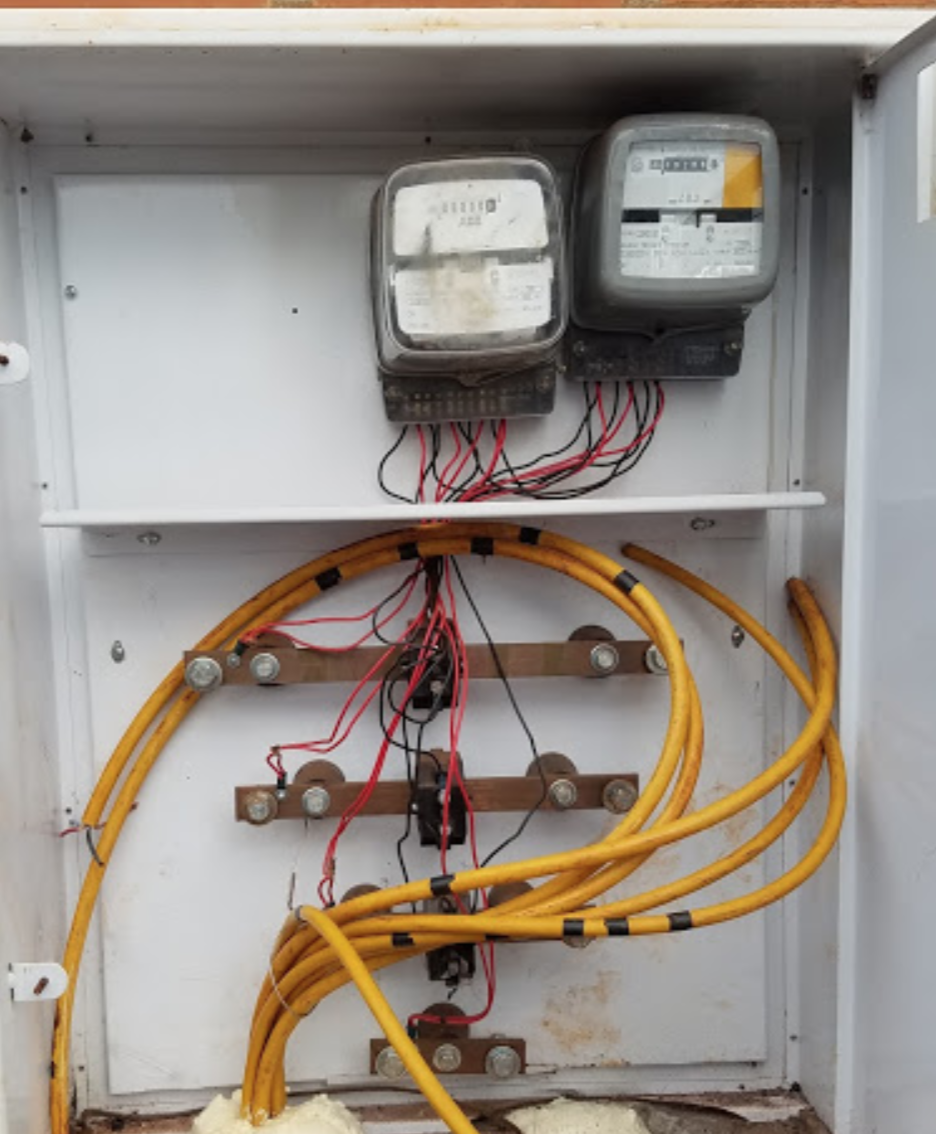
\includegraphics[width=0.5\linewidth]{Figures/Medicion_corriente_con_TI}
	\caption[]{Medición indirecta de corriente empleando transformadores de corriente (TI). Imagen tomada por el autor.}
	\label{fig:medicioncorrienteconti}
\end{figure}
La medición de corriente puede ser directa, vinculando los conductores de alimentación de la carga directamente al medidor o indirecta. Una medición indirecta consiste en reducir los valores de corriente de carga a través de transformadores de corriente (TI) y vincular sus secundarios al medidor \ref{fig:medicioncorrienteconti}. Este último método se emplea en casos donde la corriente calculada supera el valor permitido por el medidor de energía, por lo que será necesario multiplicar el valor de la lectura por un coeficiente correspondiente a la relación de transformación del TI.\\
% TODO: \usepackage{graphicx} required
\begin{figure}
	\centering
	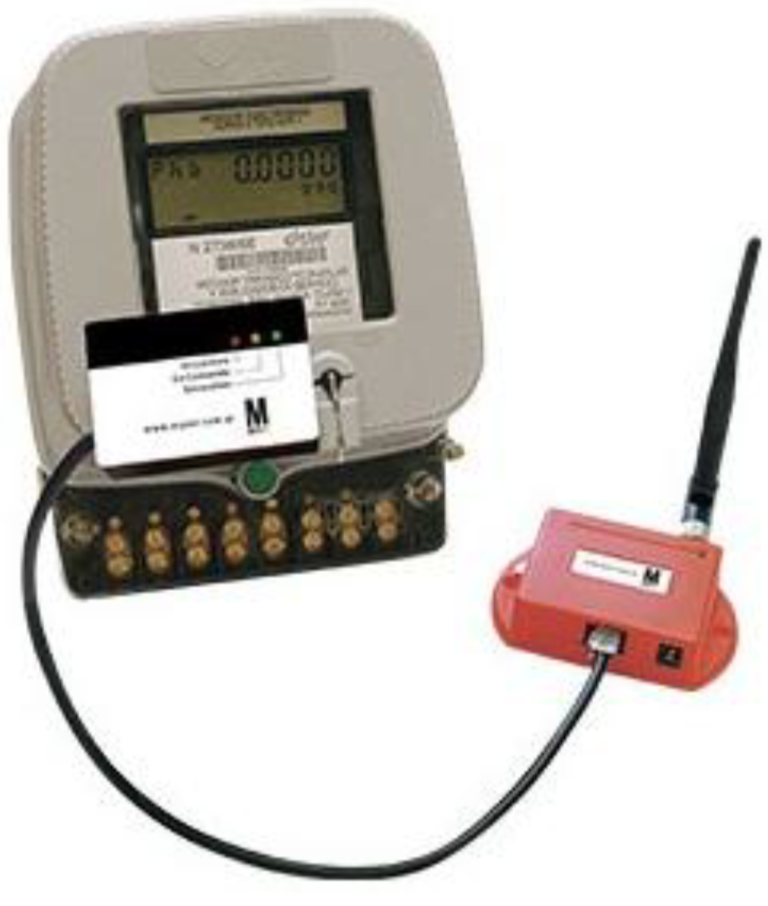
\includegraphics[width=0.5\linewidth]{Figures/medidor_digital_con_complemento_gsm}
	\caption{Medidor de energia digital con complemento para telemedición mediante GSM. Imagen tomada de \citep{MYEEL}}
	\label{fig:medidordigitalconcomplementogsm}
\end{figure}
En la actualidad algunas prestadoras del servicio eléctrico han adoptado estrategias de medición inteligente similares a la presentada en la figura \ref{fig:medidordigitalconcomplementogsm}. En este esquema los equipos de medición se reportan a centros de operación en tiempo semi real a través de una red de comunicaciones movil como por ejemplo GSM.\\
El concepto de telemedición aporta además de lo comercial, valiosa información técnica ya que los centros de operaciones conocen en todo momento el estado del medidor con la posibilidad de detectar fallas o interrupción del servicio eléctrico.\\  
A pesar de tener resultados beneficiosos en lo económico a largo plazo e inmediato en cuanto a calidad del servicio prestado, conlleva una inversión inicial considerable que muchas empresas no están dispuestas a afrontar o no tienen los recursos suficientes para su implementación.\\
\section{Estado del arte y problematica identificada}
En Sudamérica, gran parte de las empresas distibuidoras de energía eléctrica y sus tercerizadas basan parte de sus operaciones en el contacto directo con los usuarios finales mediante reclamos para informarse acerca de interrupciones en el servicio de distribución de energía eléctrica. Una vez recibido un reclamo, la prestadora de servicios envía al grupo de operaciones especializado a recorrer el área circundante al cliente y tratar de determinar el motivo de la interrupción del servicio.\\

% TODO: \usepackage{graphicx} required
\begin{figure}[h!]
	\centering
	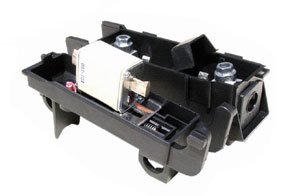
\includegraphics[width=0.7\linewidth]{Figures/NH_aereo_bt}
	\caption{Fusible seccionador aereo tipo NH usualmente utilizado en lineas de distribucion de baja tension}
	\label{fig:nh_aereo_bt}
\end{figure}
Un hecho común en el nordeste Argentino y particularmente en la provincia de Misiones es la destrucción de fusibles aéreos como el presentado en la \ref{fig:nh_aereo_bt}. Estos fusibles conectados inmediatamente a la salida de baja tension y en serie con las líneas de distribución, cumplen la función de protección por sobrecorriente debido a picos de consumo o cortocircuitos causados por desastres naturales como el de la figura \ref{fig:arbolcaidolineabt}. Los fusibles involucrados actúan de manera correcta autodestruyendose e interrumpiendo el paso de corriente.\\
\begin{figure}[h!]
	\centering
	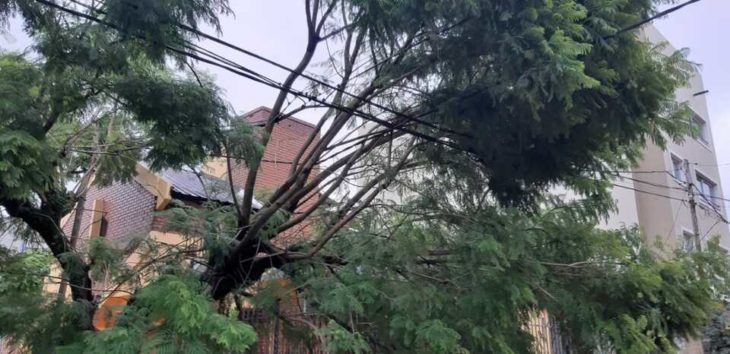
\includegraphics[width=0.7\linewidth]{Figures/arbol_caido_linea_bt}
	\caption{Un árbol caído sobre las líneas de distribución aéreas de baja tensión luego de una breve tormenta en la ciudad de Posadas, Misiones. Imagen tomada de \citep{Noticia_MNES}}
	\label{fig:arbolcaidolineabt}
\end{figure}
Este esquema presentado, resulta aún precario y no efectivo en cuanto a la rapidez para determinar la localización geográfica donde se ha generado una falla, resultando así en una inferior calidad de servicio prestada al cliente.\\

Cabe mencionar que la mayoría de las redes de distribución de baja tensión en 380/220V no poseen la capacidad de brindar algún otro servicio agregado. Algunas redes de media (33 kV) y alta tensión (132 kV) las cuales sin embargo, pueden albergar un conjunto de pelos de fibra óptica (OPGW) los cuales pueden ser utilizados para brindar servicios a terceras partes como empresas de telefonía o bien para monitoreo de la red propiamente dicha. Sin embargo, estas OPGW demuestran cierta vulnerabilidad frente a condiciones climáticas extremas tales como descargas atmosféricas y traen acarreadas un alto costo de mantenimiento \citep{ARTICLE:1}.\\
\citep{ARTICLE:2} y \citep{ARTICLE:3} comparten una arquitectura de 3 capas: física, red y aplicación para sistemas de smart grid. 
A partir del entorno donde residirá la aplicación y su objetivo final, surgen diferentes estrategias de control. Así también, la selección de sensores de diferente tipo tales como meteorológicos e infraestructura \citep{ARTICLE:3} o bien de cargas eléctricas que residen dentro de un entorno controlado haciendo uso de redes de diferente tipo \citep{ARTICLE:2}.\\
Las tecnologías emergentes propias de IoT tales como las redes de comunicación de baja potencia y largo alcance LPWAN \citep{rfc8376}, y las redes tipo malla se analizan y comparan en \citep{ARTICLE:4} como las tecnologías disponibles y viables para dotar de una infraestructura de comunicaciones a las redes de distribución metropolitanas. En \citep{ARTICLE:5} y \citep{Hua} se presentan sistemas de medición de temperatura autónomos utilizando transductores termoeléctricos y electromagnéticos para conversión de energía térmica o electromagnética en energía eléctrica para alimentar la electrónica involucrada y cargar un acumulador.

%----------------------------------------------------------------------------------------

\section{Objetivos y alcance}
\subsection{Objetivo general}
Desarrollar un sistema capaz de determinar valores eficaces de corriente alterna en sistemas metropolitanos de distribución de energía eléctrica en baja tensión y reportar estados a un centro de operaciones a través de una red LoRaWAN de acceso público.\\
\subsection{Objetivos específicos}
\begin{itemize}
	\item Evaluar el uso de un supercapacitor como reemplazo de una batería convencional.\\
	\item Desarrollar una electrónica de ultra bajo consumo para maximizar la autonomía de operación del supercapacitor.
\end{itemize}
\subsection{Alcances}
En el presente documento se desarrollan los siguientes temas:
\begin{itemize}
	\item Circuito de conversión de energía  basado en rectificadores de alta eficiencia.
	\item Acumulador de energía basado en supercapacitores
	\item Patrón de firmware implementado en el microcontrolador para optimizar el uso de energía del acumulador.
	\item Medición de valor RMS de corriente mediante transformador de corriente.
	\item Tecnología LoRaWAN
	\item Recuperación, almacenamiento y presentación de datos generados por los nodos finales.
\end{itemize}
Si bien el proyecto es parte de un plan de una PyME del autor, no  es parte del alcance ni se cubren en este documento las etapa de lanzamiento de producto ni creación de la empresa.
\subsection{Carpetas}

Esta plantilla se distribuye como una único archivo .zip que se puede descomprimir en varios archivos y carpetas. Asimismo, se puede consultar el repositorio git para obtener la última versión de los archivos, \url{https://github.com/patriciobos/Plantilla-CESE.git}. Los nombres de las carpetas son, o pretender ser, auto-explicativos.

\keyword{Appendices} -- Esta es la carpeta donde se deben poner los apéndices. Cada apéndice debe ir en su propio archivo \file{.tex}. Se incluye un ejemplo y una plantilla en la carpeta.

\keyword{Chapters} -- Esta es la carpeta donde se deben poner los capítulos de la memoria. Cada capítulo debe ir un su propio archivo \file{.tex} por separado.  Se ofrece por defecto, la siguiente estructura de capítulos y se recomienda su utilización dentro de lo posible:

\begin{itemize}
\item Capítulo 1: Introducción general	
\item Capítulo 2: Introducción específica
\item Capítulo 3: Diseño e implementación
\item Capítulo 4: Ensayos y resultados
\item Capítulo 5: Conclusiones

\end{itemize}

Esta estructura de capítulos es la que se recomienda para las memorias de la especialización.

\keyword{Figures} -- Esta carpeta contiene todas las figuras de la memoria.  Estas son las versiones finales de las imágenes que van a ser incluidas en la memoria.  Pueden ser imágenes en formato \textit{raster}\footnote{\url{https://en.wikipedia.org/wiki/Raster_graphics}} como \file{.png}, \file{.jpg} o en formato vectoriales\footnote{\url{https://en.wikipedia.org/wiki/Vector_graphics}} como \file{.pdf}, \file{.ps}.  Se debe notar que utilizar imágenes vectoriales disminuye notablemente el peso del documento final y acelera el tiempo de compilación por lo que es recomendable su utilización siempre que sea posible.

\subsection{Archivos}

También están incluidos varios archivos, la mayoría de ellos son de texto plano y se puede ver su contenido en un editor de texto. Después de la compilación inicial, se verá que más archivos auxiliares son creados por \ LaTeX{} o BibTeX, pero son de uso interno y no es necesario hacer nada en particular con ellos.  Toda la información necesaria para compilar el documento se encuentra en los archivos \file{.tex}, \file{.bib}, \file{.cls} y en las imágenes de la carpeta Figures.

\keyword{referencias.bib} - este es un archivo importante que contiene toda la información de referencias bibliográficas que se utilizarán para las citas en la memoria en conjunto con BibTeX. Usted puede escribir las entradas bibliográficas en forma manual, aunque existen también programas de gestión de referencias que facilitan la creación y gestión de las referencias y permiten exportarlas en formato BibTeX.  También hay disponibles sitios web como \url{books.google.com} que permiten obtener toda la información necesaria para una cita en formato BibTeX. Ver sección \ref{sec:biblio}

\keyword{MastersDoctoralThesis.cls} -- este es un archivo importante. Es el archivos con la clase que le informa a \LaTeX{} cómo debe dar formato a la memoria. El usuario de la plantilla no debería necesitar modificar nada de este archivo.

\keyword{memoria.pdf} -- esta es su memoria con una tipografía bellamente compuesta (en formato de archivo PDF) creado por \LaTeX{}. Se distribuye con la plantilla y después de compilar por primera vez sin hacer ningún cambio se debería obtener una versión idéntica a este documento.

\keyword{memoria.tex} -- este es un archivo importante. Este es el archivo que tiene que compilar \LaTeX{} para producir la memoria como un archivo PDF. Contiene un marco de trabajo y estructuras que le indican a \LaTeX{} cómo diagramar la memoria.  Está altamente comentado para que se pueda entender qué es lo que realiza cada línea de código y por qué está incluida en ese lugar.  En este archivo se debe completar la información personalizada de las primeras sección según se indica en la sección \ref{sec:FillingFile}.

Archivos que \emph{no} forman parte de la distribución de la plantilla pero que son generados por \LaTeX{} como archivos auxiliares necesarios para la producción de la memoria.pdf son:

\keyword{memoria.aux} -- este es un archivo auxiliar generado por \LaTeX{}, si se borra \LaTeX{} simplemente lo regenera cuando se compila el archivo principal \file{memoria.tex}.

\keyword{memoria.bbl} -- este es un archivo auxiliar generado por BibTeX, si se borra BibTeX simplemente lo regenera cuando se compila el archivo principal \file{memoria.tex}. Mientras que el archivo \file{.bib} contiene todas las referencias que hay, este archivo \file{.bbl} contine sólo las referencias que han sido citadas y se utiliza para la construcción de la bibiografía.

\keyword{memoria.blg} -- este es un archivo auxiliar generado por BibTeX, si se borra BibTeX simplemente lo regenera cuando se compila el archivo principal \file{memoria.tex}.

\keyword{memoria.lof} -- este es un archivo auxiliar generado por \LaTeX{}, si se borra \LaTeX{} simplemente lo regenera cuando se compila el archivo principal \file{memoria.tex}.  Le indica a \LaTeX{} cómo construir la sección \emph{Lista de Figuras}.
 
\keyword{memoria.log} --  este es un archivo auxiliar generado por \LaTeX{}, si se borra \LaTeX{} simplemente lo regenera cuando se compila el archivo principal \file{memoria.tex}. Contiene mensajes de \LaTeX{}. Si se reciben errores o advertencias durante la compilación, se guardan en este archivo \file{.log}.

\keyword{memoria.lot} -- este es un archivo auxiliar generado por \LaTeX{}, si se borra \LaTeX{} simplemente lo regenera cuando se compila el archivo principal \file{memoria.tex}.  Le indica a \LaTeX{} cómo construir la sección \emph{Lista de Tablas}.

\keyword{memoria.out} -- este es un archivo auxiliar generado por \LaTeX{}, si se borra \LaTeX{} simplemente lo regenera cuando se compila el archivo principal \file{memoria.tex}.

De esta larga lista de archivos, sólo aquellos con la extensión \file{.bib}, \file{.cls} y \file{.tex} son importantes.  Los otros archivos auxiliares pueden ser ignorados o borrados ya que \LaTeX{} y BibTeX los regenerarán durante la compilación.

%----------------------------------------------------------------------------------------

\section{Entorno de trabajo}

Ante de comenzar a editar la plantilla debemos tener un editor \LaTeX{} instalado en nuestra computadora.  En forma análoga a lo que sucede en lenguaje C, que se puede crear y editar código con casi cualquier editor, existen ciertos entornos de trabajo que nos pueden simplificar mucho la tarea.  En este sentido, se recomienda, sobre todo para los principiantes en \LaTeX{} la utilización de TexMaker, un programa gratuito y multi-plantaforma que está disponible tanto para windows como para sistemas GNU/linux.

La versión más reciente de TexMaker es la 4.5 y se puede descargar del siguiente link: \url{http://www.xm1math.net/texmaker/download.html}. Se puede consultar el manual de usuario en el siguiente link: \url{http://www.xm1math.net/texmaker/doc.html}.
 

\subsection{Paquetes adicionales}

Si bien durante el proceso de instalación de TexMaker, o cualquier otro editor que se haya elegido, se instalarán en el sistema los paquetes básicos necesarios para trabajar con \LaTeX{}, la plantilla de los trabajos de Especialización y Maestría requieren de paquete adicionales.

Se indican a continuación los comandos que se deben introducir en la consola de Ubuntu (ctrl + alt + t) para instalarlos:

\begin{lstlisting}[language=bash]
  $ sudo apt install texlive-lang-spanish texlive-science 
  $ sudo apt install texlive-bibtex-extra biber
  $ sudo apt install texlive texlive-fonts-recommended
  $ sudo apt install texlive-latex-extra
\end{lstlisting}


\subsection{Configurando TexMaker}


Una vez instalado el programa y los paquetes adicionales se debe abrir el archivo memoria.tex con el editor para ver una pantalla similar a la que se puede apreciar en la figura \ref{fig:texmaker}. 

\begin{figure}[h]
	\centering
	\includegraphics[width=\textwidth]{./Figures/texmaker.png}
	\caption{Entorno de trabajo de texMaker.}
	\label{fig:texmaker}
\end{figure}

Notar que existe una vista llamada Estructura a la izquierda de la interfaz que nos permite abrir desde dentro del programa los archivos individuales de los capítulos.  A la derecha se encuentra una vista con el archivo propiamente dicho para su edición. Hacia la parte inferior se encuentra una vista del log con información de los resultados de la compilación.  En esta última vista pueden aparecen advertencias o \textit{warning}, que normalmente pueden ser ignorados, y los errores que se indican en color rojo y deben resolverse para que se genere el PDF de salida.

Recordar que el archivo que se debe compilar con PDFLaTeX es \file{memoria.tex}, si se tratara de compilar alguno de los capítulos saldría un error.  Para salvar la molestia de tener que cambiar de archivo para compilar cada vez que se realice una modificación en un capítulo, se puede definir el archivo \file{memoria.tex} como ``documento maestro'' yendo al menú opciones -> ``definir documento actual como documento maestro'', lo que permite compilar con PDFLaTeX memoria.tex directamente desde cualquier archivo que se esté modificando . Se muestra esta opción en la figura \ref{fig:docMaestro}.

\begin{figure}[h]
	\centering
	\includegraphics[width=\textwidth]{./Figures/docMaestro.png}
	\caption{Definir memoria.tex como documento maestro.}
	\label{fig:docMaestro}
\end{figure}

En el menú herramientas se encuentran las opciones de compilación.  Para producir un archivo PDF a partir de un archivo .tex se debe ejecutar PDFLaTeX (el shortcut es F6). Para incorporar nueva bibliografía se debe utilizar la opción BibTeX del mismo menú herramientas (el shortcut es F11).

Notar que para actualizar las tablas de contenidos se debe ejecutar PDFLaTeX dos veces.  Esto se debe a que es necesario actualizar algunos archivos auxiliares antes de obtener el resultado final.  En forma similar, para actualizar las referencias se debe ejecutar primero PDFLaTeX, después BibTeX y finalmente PDFLaTeX dos veces por idénticos motivos.

\section{Personalizando la plantilla, el archivo \file{memoria.tex}}
\label{sec:FillingFile}

Para personalizar la plantilla se debe incorporar la información propia en los distintos archivos \file{.tex}. 

Primero abrir \file{memoria.tex} con TexMaker (o el editor de su preferencia). Se debe ubicar dentro del archivo el bloque de código titulado \emph{INFORMACIÓN DE LA PORTADA} donde se deben incorporar los primeros datos personales con los que se construirá automáticamente la portada.


%----------------------------------------------------------------------------------------

\section{El código del archivo \file{memoria.tex} explicado}

El archivo \file{memoria.tex} contiene la estructura del documento y es el archivo de mayor jerarquía de la memoria.  Podría ser equiparable a la función \emph{main()} de un programa en C, o mejor dicho al archivo fuente .c donde se encuentra definida la función main().

La estructura básica de cualquier documento de \LaTeX{} comienza con la definición de clase del documento, es seguida por un preámbulo donde se pueden agregar funcionalidades con el uso de \texttt{paquetes} (equiparables a bibliotecas de C), y finalmente, termina con el cuerpo del documento, donde irá el contenido de la memoria.

\lstset{%
  basicstyle=\small\ttfamily,
  language=[LaTeX]{TeX}
}

\begin{lstlisting}
\documentclass{article}  <- Definicion de clase
\usepackage{listings}	 <- Preambulo

\begin{document}	 <- Comienzo del contenido propio 
	Hello world!
\end{document}
\end{lstlisting}


El archivo \file{memoria.tex} se encuentra densamente comentado para explicar qué páginas, secciones y elementos de formato está creando el código \LaTeX{} en cada línea. El código está dividido en bloques con nombres en mayúsculas para que resulte evidente qué es lo que hace esa porción de código en particular. Inicialmente puede parecer que hay mucho código \LaTeX{}, pero es principalmente código para dar formato a la memoria por lo que no requiere intervención del usuario de la plantilla.  Sí se deben personalizar con su información los bloques indicados como:

\begin{itemize}
	\item Informacion de la memoria
	\item Resumen
	\item Agradecimientos
	\item Dedicatoria
\end{itemize}

El índice de contenidos, las listas de figura de tablas se generan en forma automática y no requieren intervención ni edición manual por parte del usuario de la plantilla. 

En la parte final del documento se encuentran los capítulos y los apéndices.  Por defecto se incluyen los 5 capítulos propuestos que se encuentran en la carpeta /Chapters. Cada capítulo se debe escribir en un archivo .tex separado y se debe poner en la carpeta \emph{Chapters} con el nombre \file{Chapter1}, \file{Chapter2}, etc\ldots El código para incluir capítulos desde archivos externos se muestra a continuación.

\begin{verbatim}
	% Chapter 1
\chapter{Introducción general} % Main chapter title

\label{Chapter1} % For referencing the chapter elsewhere, use \ref{Chapter1} 
\label{IntroGeneral}

%----------------------------------------------------------------------------------------

% Define some commands to keep the formatting separated from the content 
\newcommand{\keyword}[1]{\textbf{#1}}
\newcommand{\tabhead}[1]{\textbf{#1}}
\newcommand{\code}[1]{\texttt{#1}}
\newcommand{\file}[1]{\texttt{\bfseries#1}}
\newcommand{\option}[1]{\texttt{\itshape#1}}
\newcommand{\grados}{$^{\circ}$}

%----------------------------------------------------------------------------------------

%\section{Introducción}

%----------------------------------------------------------------------------------------
\section{Estaciones transformadoras}

Se denomina estación transformadora al conjunto de equipos electromecánicos responsables de convertir la energía eléctrica variando uno o más de sus principales parámetros que son tensión y corriente, a través del componente más importante del conjunto que es el transformador. La finalidad de convertir la energía eléctrica, que puede ser elevando o reduciendo el nivel de tensión, es poder transmitir y distribuir esa energía hacia los receptores que pueden ser consumidores finales tales como residencias familiares o los denominados grandes usuarios por ejemplo industrias.\\

Por convención se denomina Estación Transformadora (E.T.) cuando en el proceso se ven involucrados valores considerados de alta tensión (mayor a 66 kV) y Subestación Transformadora (S.E.T.) en el caso de tensiones menores a 66 kV \citep{AEA:1}.\\
Para la distribución hacia los consumidores finales, se utilizan las denominadas Subestaciones Transformadoras Aéreas (S.E.T.A.) que convierten la tensión disminuyendo su valor de media a baja tensión.\\

Para poder obtener energía eléctrica a la salida en óptimas condiciones de calidad y disponibilidad, resulta fundamental administrar y controlar los valores intrínsecos que componen la transmisión y recepción de la misma. Esto se logra a través de instrumentos de medición de tensión y corriente, tanto a la entrada (alta tensión) como a la salida (media tensión) de la conversión. Por otro lado y con el fin de mantener y preservar los equipos electromecánicos se consideran de gran importancia otros valores físicos como ser temperatura y humedad.\\

\section{Medidores de energía}
Llegado el momento de entregar la energía al usuario final, es indispensable cuantificarla para luego comercializarla. Las distribuidoras del servicio utilizan medidores de energía de electromecánicos o electrónicos, que registran en todo momento la energía acumulada que fluye por el mismo.\\
% TODO: \usepackage{graphicx} required
\begin{figure}
	\centering
	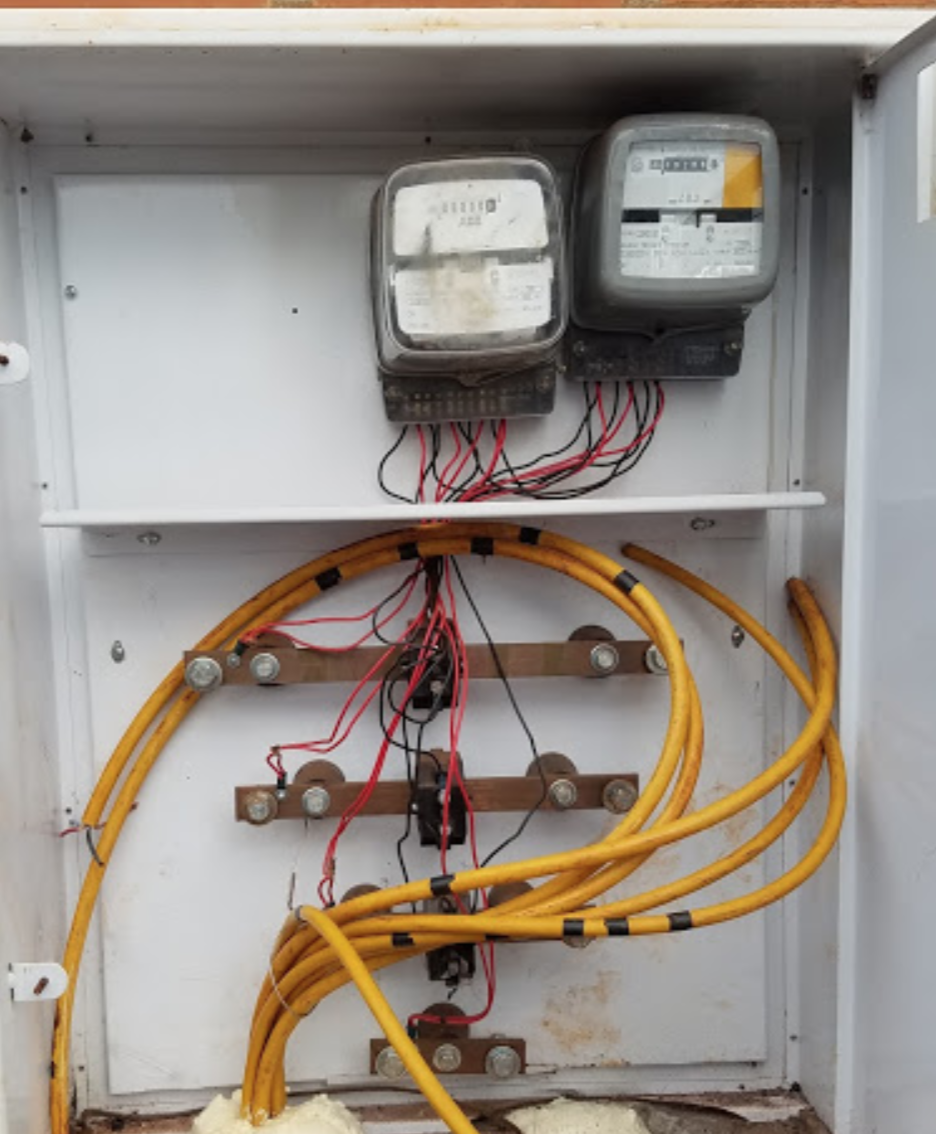
\includegraphics[width=0.5\linewidth]{Figures/Medicion_corriente_con_TI}
	\caption[]{Medición indirecta de corriente empleando transformadores de corriente (TI). Imagen tomada por el autor.}
	\label{fig:medicioncorrienteconti}
\end{figure}
La medición de corriente puede ser directa, vinculando los conductores de alimentación de la carga directamente al medidor o indirecta. Una medición indirecta consiste en reducir los valores de corriente de carga a través de transformadores de corriente (TI) y vincular sus secundarios al medidor \ref{fig:medicioncorrienteconti}. Este último método se emplea en casos donde la corriente calculada supera el valor permitido por el medidor de energía, por lo que será necesario multiplicar el valor de la lectura por un coeficiente correspondiente a la relación de transformación del TI.\\
% TODO: \usepackage{graphicx} required
\begin{figure}
	\centering
	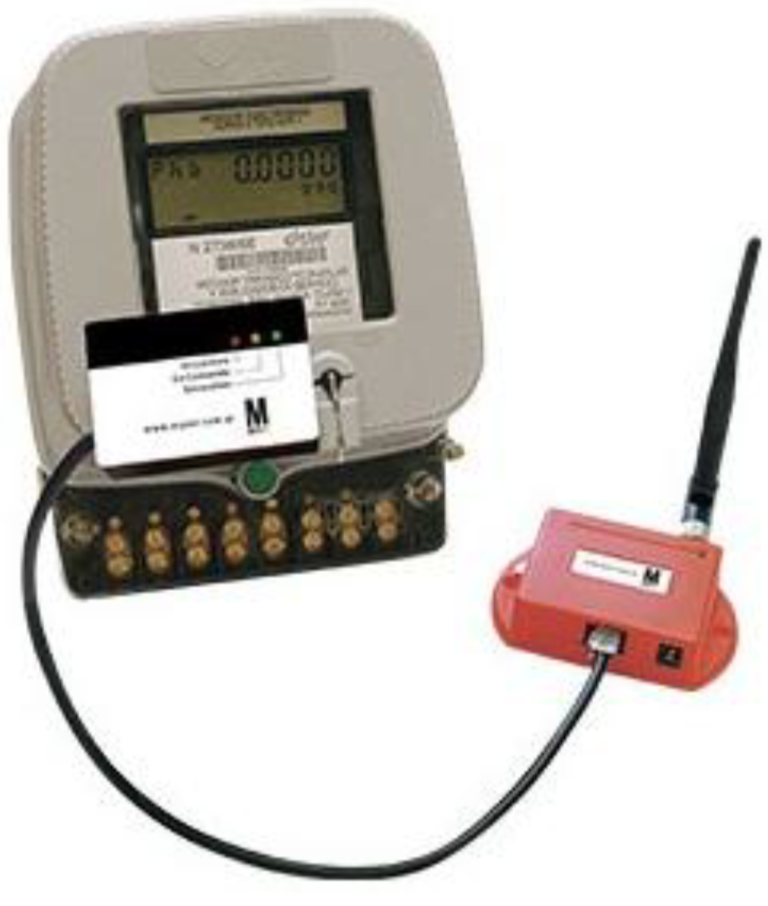
\includegraphics[width=0.5\linewidth]{Figures/medidor_digital_con_complemento_gsm}
	\caption{Medidor de energia digital con complemento para telemedición mediante GSM. Imagen tomada de \citep{MYEEL}}
	\label{fig:medidordigitalconcomplementogsm}
\end{figure}
En la actualidad algunas prestadoras del servicio eléctrico han adoptado estrategias de medición inteligente similares a la presentada en la figura \ref{fig:medidordigitalconcomplementogsm}. En este esquema los equipos de medición se reportan a centros de operación en tiempo semi real a través de una red de comunicaciones movil como por ejemplo GSM.\\
El concepto de telemedición aporta además de lo comercial, valiosa información técnica ya que los centros de operaciones conocen en todo momento el estado del medidor con la posibilidad de detectar fallas o interrupción del servicio eléctrico.\\  
A pesar de tener resultados beneficiosos en lo económico a largo plazo e inmediato en cuanto a calidad del servicio prestado, conlleva una inversión inicial considerable que muchas empresas no están dispuestas a afrontar o no tienen los recursos suficientes para su implementación.\\
\section{Estado del arte y problematica identificada}
En Sudamérica, gran parte de las empresas distibuidoras de energía eléctrica y sus tercerizadas basan parte de sus operaciones en el contacto directo con los usuarios finales mediante reclamos para informarse acerca de interrupciones en el servicio de distribución de energía eléctrica. Una vez recibido un reclamo, la prestadora de servicios envía al grupo de operaciones especializado a recorrer el área circundante al cliente y tratar de determinar el motivo de la interrupción del servicio.\\

% TODO: \usepackage{graphicx} required
\begin{figure}[h!]
	\centering
	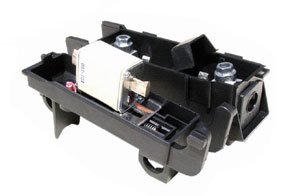
\includegraphics[width=0.7\linewidth]{Figures/NH_aereo_bt}
	\caption{Fusible seccionador aereo tipo NH usualmente utilizado en lineas de distribucion de baja tension}
	\label{fig:nh_aereo_bt}
\end{figure}
Un hecho común en el nordeste Argentino y particularmente en la provincia de Misiones es la destrucción de fusibles aéreos como el presentado en la \ref{fig:nh_aereo_bt}. Estos fusibles conectados inmediatamente a la salida de baja tension y en serie con las líneas de distribución, cumplen la función de protección por sobrecorriente debido a picos de consumo o cortocircuitos causados por desastres naturales como el de la figura \ref{fig:arbolcaidolineabt}. Los fusibles involucrados actúan de manera correcta autodestruyendose e interrumpiendo el paso de corriente.\\
\begin{figure}[h!]
	\centering
	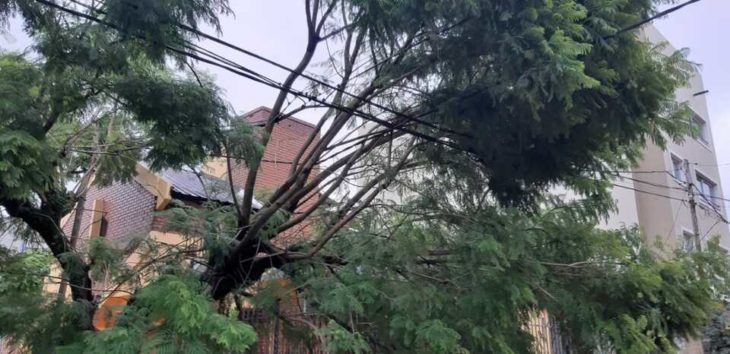
\includegraphics[width=0.7\linewidth]{Figures/arbol_caido_linea_bt}
	\caption{Un árbol caído sobre las líneas de distribución aéreas de baja tensión luego de una breve tormenta en la ciudad de Posadas, Misiones. Imagen tomada de \citep{Noticia_MNES}}
	\label{fig:arbolcaidolineabt}
\end{figure}
Este esquema presentado, resulta aún precario y no efectivo en cuanto a la rapidez para determinar la localización geográfica donde se ha generado una falla, resultando así en una inferior calidad de servicio prestada al cliente.\\

Cabe mencionar que la mayoría de las redes de distribución de baja tensión en 380/220V no poseen la capacidad de brindar algún otro servicio agregado. Algunas redes de media (33 kV) y alta tensión (132 kV) las cuales sin embargo, pueden albergar un conjunto de pelos de fibra óptica (OPGW) los cuales pueden ser utilizados para brindar servicios a terceras partes como empresas de telefonía o bien para monitoreo de la red propiamente dicha. Sin embargo, estas OPGW demuestran cierta vulnerabilidad frente a condiciones climáticas extremas tales como descargas atmosféricas y traen acarreadas un alto costo de mantenimiento \citep{ARTICLE:1}.\\
\citep{ARTICLE:2} y \citep{ARTICLE:3} comparten una arquitectura de 3 capas: física, red y aplicación para sistemas de smart grid. 
A partir del entorno donde residirá la aplicación y su objetivo final, surgen diferentes estrategias de control. Así también, la selección de sensores de diferente tipo tales como meteorológicos e infraestructura \citep{ARTICLE:3} o bien de cargas eléctricas que residen dentro de un entorno controlado haciendo uso de redes de diferente tipo \citep{ARTICLE:2}.\\
Las tecnologías emergentes propias de IoT tales como las redes de comunicación de baja potencia y largo alcance LPWAN \citep{rfc8376}, y las redes tipo malla se analizan y comparan en \citep{ARTICLE:4} como las tecnologías disponibles y viables para dotar de una infraestructura de comunicaciones a las redes de distribución metropolitanas. En \citep{ARTICLE:5} y \citep{Hua} se presentan sistemas de medición de temperatura autónomos utilizando transductores termoeléctricos y electromagnéticos para conversión de energía térmica o electromagnética en energía eléctrica para alimentar la electrónica involucrada y cargar un acumulador.

%----------------------------------------------------------------------------------------

\section{Objetivos y alcance}
\subsection{Objetivo general}
Desarrollar un sistema capaz de determinar valores eficaces de corriente alterna en sistemas metropolitanos de distribución de energía eléctrica en baja tensión y reportar estados a un centro de operaciones a través de una red LoRaWAN de acceso público.\\
\subsection{Objetivos específicos}
\begin{itemize}
	\item Evaluar el uso de un supercapacitor como reemplazo de una batería convencional.\\
	\item Desarrollar una electrónica de ultra bajo consumo para maximizar la autonomía de operación del supercapacitor.
\end{itemize}
\subsection{Alcances}
En el presente documento se desarrollan los siguientes temas:
\begin{itemize}
	\item Circuito de conversión de energía  basado en rectificadores de alta eficiencia.
	\item Acumulador de energía basado en supercapacitores
	\item Patrón de firmware implementado en el microcontrolador para optimizar el uso de energía del acumulador.
	\item Medición de valor RMS de corriente mediante transformador de corriente.
	\item Tecnología LoRaWAN
	\item Recuperación, almacenamiento y presentación de datos generados por los nodos finales.
\end{itemize}
Si bien el proyecto es parte de un plan de una PyME del autor, no  es parte del alcance ni se cubren en este documento las etapa de lanzamiento de producto ni creación de la empresa.
\subsection{Carpetas}

Esta plantilla se distribuye como una único archivo .zip que se puede descomprimir en varios archivos y carpetas. Asimismo, se puede consultar el repositorio git para obtener la última versión de los archivos, \url{https://github.com/patriciobos/Plantilla-CESE.git}. Los nombres de las carpetas son, o pretender ser, auto-explicativos.

\keyword{Appendices} -- Esta es la carpeta donde se deben poner los apéndices. Cada apéndice debe ir en su propio archivo \file{.tex}. Se incluye un ejemplo y una plantilla en la carpeta.

\keyword{Chapters} -- Esta es la carpeta donde se deben poner los capítulos de la memoria. Cada capítulo debe ir un su propio archivo \file{.tex} por separado.  Se ofrece por defecto, la siguiente estructura de capítulos y se recomienda su utilización dentro de lo posible:

\begin{itemize}
\item Capítulo 1: Introducción general	
\item Capítulo 2: Introducción específica
\item Capítulo 3: Diseño e implementación
\item Capítulo 4: Ensayos y resultados
\item Capítulo 5: Conclusiones

\end{itemize}

Esta estructura de capítulos es la que se recomienda para las memorias de la especialización.

\keyword{Figures} -- Esta carpeta contiene todas las figuras de la memoria.  Estas son las versiones finales de las imágenes que van a ser incluidas en la memoria.  Pueden ser imágenes en formato \textit{raster}\footnote{\url{https://en.wikipedia.org/wiki/Raster_graphics}} como \file{.png}, \file{.jpg} o en formato vectoriales\footnote{\url{https://en.wikipedia.org/wiki/Vector_graphics}} como \file{.pdf}, \file{.ps}.  Se debe notar que utilizar imágenes vectoriales disminuye notablemente el peso del documento final y acelera el tiempo de compilación por lo que es recomendable su utilización siempre que sea posible.

\subsection{Archivos}

También están incluidos varios archivos, la mayoría de ellos son de texto plano y se puede ver su contenido en un editor de texto. Después de la compilación inicial, se verá que más archivos auxiliares son creados por \ LaTeX{} o BibTeX, pero son de uso interno y no es necesario hacer nada en particular con ellos.  Toda la información necesaria para compilar el documento se encuentra en los archivos \file{.tex}, \file{.bib}, \file{.cls} y en las imágenes de la carpeta Figures.

\keyword{referencias.bib} - este es un archivo importante que contiene toda la información de referencias bibliográficas que se utilizarán para las citas en la memoria en conjunto con BibTeX. Usted puede escribir las entradas bibliográficas en forma manual, aunque existen también programas de gestión de referencias que facilitan la creación y gestión de las referencias y permiten exportarlas en formato BibTeX.  También hay disponibles sitios web como \url{books.google.com} que permiten obtener toda la información necesaria para una cita en formato BibTeX. Ver sección \ref{sec:biblio}

\keyword{MastersDoctoralThesis.cls} -- este es un archivo importante. Es el archivos con la clase que le informa a \LaTeX{} cómo debe dar formato a la memoria. El usuario de la plantilla no debería necesitar modificar nada de este archivo.

\keyword{memoria.pdf} -- esta es su memoria con una tipografía bellamente compuesta (en formato de archivo PDF) creado por \LaTeX{}. Se distribuye con la plantilla y después de compilar por primera vez sin hacer ningún cambio se debería obtener una versión idéntica a este documento.

\keyword{memoria.tex} -- este es un archivo importante. Este es el archivo que tiene que compilar \LaTeX{} para producir la memoria como un archivo PDF. Contiene un marco de trabajo y estructuras que le indican a \LaTeX{} cómo diagramar la memoria.  Está altamente comentado para que se pueda entender qué es lo que realiza cada línea de código y por qué está incluida en ese lugar.  En este archivo se debe completar la información personalizada de las primeras sección según se indica en la sección \ref{sec:FillingFile}.

Archivos que \emph{no} forman parte de la distribución de la plantilla pero que son generados por \LaTeX{} como archivos auxiliares necesarios para la producción de la memoria.pdf son:

\keyword{memoria.aux} -- este es un archivo auxiliar generado por \LaTeX{}, si se borra \LaTeX{} simplemente lo regenera cuando se compila el archivo principal \file{memoria.tex}.

\keyword{memoria.bbl} -- este es un archivo auxiliar generado por BibTeX, si se borra BibTeX simplemente lo regenera cuando se compila el archivo principal \file{memoria.tex}. Mientras que el archivo \file{.bib} contiene todas las referencias que hay, este archivo \file{.bbl} contine sólo las referencias que han sido citadas y se utiliza para la construcción de la bibiografía.

\keyword{memoria.blg} -- este es un archivo auxiliar generado por BibTeX, si se borra BibTeX simplemente lo regenera cuando se compila el archivo principal \file{memoria.tex}.

\keyword{memoria.lof} -- este es un archivo auxiliar generado por \LaTeX{}, si se borra \LaTeX{} simplemente lo regenera cuando se compila el archivo principal \file{memoria.tex}.  Le indica a \LaTeX{} cómo construir la sección \emph{Lista de Figuras}.
 
\keyword{memoria.log} --  este es un archivo auxiliar generado por \LaTeX{}, si se borra \LaTeX{} simplemente lo regenera cuando se compila el archivo principal \file{memoria.tex}. Contiene mensajes de \LaTeX{}. Si se reciben errores o advertencias durante la compilación, se guardan en este archivo \file{.log}.

\keyword{memoria.lot} -- este es un archivo auxiliar generado por \LaTeX{}, si se borra \LaTeX{} simplemente lo regenera cuando se compila el archivo principal \file{memoria.tex}.  Le indica a \LaTeX{} cómo construir la sección \emph{Lista de Tablas}.

\keyword{memoria.out} -- este es un archivo auxiliar generado por \LaTeX{}, si se borra \LaTeX{} simplemente lo regenera cuando se compila el archivo principal \file{memoria.tex}.

De esta larga lista de archivos, sólo aquellos con la extensión \file{.bib}, \file{.cls} y \file{.tex} son importantes.  Los otros archivos auxiliares pueden ser ignorados o borrados ya que \LaTeX{} y BibTeX los regenerarán durante la compilación.

%----------------------------------------------------------------------------------------

\section{Entorno de trabajo}

Ante de comenzar a editar la plantilla debemos tener un editor \LaTeX{} instalado en nuestra computadora.  En forma análoga a lo que sucede en lenguaje C, que se puede crear y editar código con casi cualquier editor, existen ciertos entornos de trabajo que nos pueden simplificar mucho la tarea.  En este sentido, se recomienda, sobre todo para los principiantes en \LaTeX{} la utilización de TexMaker, un programa gratuito y multi-plantaforma que está disponible tanto para windows como para sistemas GNU/linux.

La versión más reciente de TexMaker es la 4.5 y se puede descargar del siguiente link: \url{http://www.xm1math.net/texmaker/download.html}. Se puede consultar el manual de usuario en el siguiente link: \url{http://www.xm1math.net/texmaker/doc.html}.
 

\subsection{Paquetes adicionales}

Si bien durante el proceso de instalación de TexMaker, o cualquier otro editor que se haya elegido, se instalarán en el sistema los paquetes básicos necesarios para trabajar con \LaTeX{}, la plantilla de los trabajos de Especialización y Maestría requieren de paquete adicionales.

Se indican a continuación los comandos que se deben introducir en la consola de Ubuntu (ctrl + alt + t) para instalarlos:

\begin{lstlisting}[language=bash]
  $ sudo apt install texlive-lang-spanish texlive-science 
  $ sudo apt install texlive-bibtex-extra biber
  $ sudo apt install texlive texlive-fonts-recommended
  $ sudo apt install texlive-latex-extra
\end{lstlisting}


\subsection{Configurando TexMaker}


Una vez instalado el programa y los paquetes adicionales se debe abrir el archivo memoria.tex con el editor para ver una pantalla similar a la que se puede apreciar en la figura \ref{fig:texmaker}. 

\begin{figure}[h]
	\centering
	\includegraphics[width=\textwidth]{./Figures/texmaker.png}
	\caption{Entorno de trabajo de texMaker.}
	\label{fig:texmaker}
\end{figure}

Notar que existe una vista llamada Estructura a la izquierda de la interfaz que nos permite abrir desde dentro del programa los archivos individuales de los capítulos.  A la derecha se encuentra una vista con el archivo propiamente dicho para su edición. Hacia la parte inferior se encuentra una vista del log con información de los resultados de la compilación.  En esta última vista pueden aparecen advertencias o \textit{warning}, que normalmente pueden ser ignorados, y los errores que se indican en color rojo y deben resolverse para que se genere el PDF de salida.

Recordar que el archivo que se debe compilar con PDFLaTeX es \file{memoria.tex}, si se tratara de compilar alguno de los capítulos saldría un error.  Para salvar la molestia de tener que cambiar de archivo para compilar cada vez que se realice una modificación en un capítulo, se puede definir el archivo \file{memoria.tex} como ``documento maestro'' yendo al menú opciones -> ``definir documento actual como documento maestro'', lo que permite compilar con PDFLaTeX memoria.tex directamente desde cualquier archivo que se esté modificando . Se muestra esta opción en la figura \ref{fig:docMaestro}.

\begin{figure}[h]
	\centering
	\includegraphics[width=\textwidth]{./Figures/docMaestro.png}
	\caption{Definir memoria.tex como documento maestro.}
	\label{fig:docMaestro}
\end{figure}

En el menú herramientas se encuentran las opciones de compilación.  Para producir un archivo PDF a partir de un archivo .tex se debe ejecutar PDFLaTeX (el shortcut es F6). Para incorporar nueva bibliografía se debe utilizar la opción BibTeX del mismo menú herramientas (el shortcut es F11).

Notar que para actualizar las tablas de contenidos se debe ejecutar PDFLaTeX dos veces.  Esto se debe a que es necesario actualizar algunos archivos auxiliares antes de obtener el resultado final.  En forma similar, para actualizar las referencias se debe ejecutar primero PDFLaTeX, después BibTeX y finalmente PDFLaTeX dos veces por idénticos motivos.

\section{Personalizando la plantilla, el archivo \file{memoria.tex}}
\label{sec:FillingFile}

Para personalizar la plantilla se debe incorporar la información propia en los distintos archivos \file{.tex}. 

Primero abrir \file{memoria.tex} con TexMaker (o el editor de su preferencia). Se debe ubicar dentro del archivo el bloque de código titulado \emph{INFORMACIÓN DE LA PORTADA} donde se deben incorporar los primeros datos personales con los que se construirá automáticamente la portada.


%----------------------------------------------------------------------------------------

\section{El código del archivo \file{memoria.tex} explicado}

El archivo \file{memoria.tex} contiene la estructura del documento y es el archivo de mayor jerarquía de la memoria.  Podría ser equiparable a la función \emph{main()} de un programa en C, o mejor dicho al archivo fuente .c donde se encuentra definida la función main().

La estructura básica de cualquier documento de \LaTeX{} comienza con la definición de clase del documento, es seguida por un preámbulo donde se pueden agregar funcionalidades con el uso de \texttt{paquetes} (equiparables a bibliotecas de C), y finalmente, termina con el cuerpo del documento, donde irá el contenido de la memoria.

\lstset{%
  basicstyle=\small\ttfamily,
  language=[LaTeX]{TeX}
}

\begin{lstlisting}
\documentclass{article}  <- Definicion de clase
\usepackage{listings}	 <- Preambulo

\begin{document}	 <- Comienzo del contenido propio 
	Hello world!
\end{document}
\end{lstlisting}


El archivo \file{memoria.tex} se encuentra densamente comentado para explicar qué páginas, secciones y elementos de formato está creando el código \LaTeX{} en cada línea. El código está dividido en bloques con nombres en mayúsculas para que resulte evidente qué es lo que hace esa porción de código en particular. Inicialmente puede parecer que hay mucho código \LaTeX{}, pero es principalmente código para dar formato a la memoria por lo que no requiere intervención del usuario de la plantilla.  Sí se deben personalizar con su información los bloques indicados como:

\begin{itemize}
	\item Informacion de la memoria
	\item Resumen
	\item Agradecimientos
	\item Dedicatoria
\end{itemize}

El índice de contenidos, las listas de figura de tablas se generan en forma automática y no requieren intervención ni edición manual por parte del usuario de la plantilla. 

En la parte final del documento se encuentran los capítulos y los apéndices.  Por defecto se incluyen los 5 capítulos propuestos que se encuentran en la carpeta /Chapters. Cada capítulo se debe escribir en un archivo .tex separado y se debe poner en la carpeta \emph{Chapters} con el nombre \file{Chapter1}, \file{Chapter2}, etc\ldots El código para incluir capítulos desde archivos externos se muestra a continuación.

\begin{verbatim}
	% Chapter 1
\chapter{Introducción general} % Main chapter title

\label{Chapter1} % For referencing the chapter elsewhere, use \ref{Chapter1} 
\label{IntroGeneral}

%----------------------------------------------------------------------------------------

% Define some commands to keep the formatting separated from the content 
\newcommand{\keyword}[1]{\textbf{#1}}
\newcommand{\tabhead}[1]{\textbf{#1}}
\newcommand{\code}[1]{\texttt{#1}}
\newcommand{\file}[1]{\texttt{\bfseries#1}}
\newcommand{\option}[1]{\texttt{\itshape#1}}
\newcommand{\grados}{$^{\circ}$}

%----------------------------------------------------------------------------------------

%\section{Introducción}

%----------------------------------------------------------------------------------------
\section{Estaciones transformadoras}

Se denomina estación transformadora al conjunto de equipos electromecánicos responsables de convertir la energía eléctrica variando uno o más de sus principales parámetros que son tensión y corriente, a través del componente más importante del conjunto que es el transformador. La finalidad de convertir la energía eléctrica, que puede ser elevando o reduciendo el nivel de tensión, es poder transmitir y distribuir esa energía hacia los receptores que pueden ser consumidores finales tales como residencias familiares o los denominados grandes usuarios por ejemplo industrias.\\

Por convención se denomina Estación Transformadora (E.T.) cuando en el proceso se ven involucrados valores considerados de alta tensión (mayor a 66 kV) y Subestación Transformadora (S.E.T.) en el caso de tensiones menores a 66 kV \citep{AEA:1}.\\
Para la distribución hacia los consumidores finales, se utilizan las denominadas Subestaciones Transformadoras Aéreas (S.E.T.A.) que convierten la tensión disminuyendo su valor de media a baja tensión.\\

Para poder obtener energía eléctrica a la salida en óptimas condiciones de calidad y disponibilidad, resulta fundamental administrar y controlar los valores intrínsecos que componen la transmisión y recepción de la misma. Esto se logra a través de instrumentos de medición de tensión y corriente, tanto a la entrada (alta tensión) como a la salida (media tensión) de la conversión. Por otro lado y con el fin de mantener y preservar los equipos electromecánicos se consideran de gran importancia otros valores físicos como ser temperatura y humedad.\\

\section{Medidores de energía}
Llegado el momento de entregar la energía al usuario final, es indispensable cuantificarla para luego comercializarla. Las distribuidoras del servicio utilizan medidores de energía de electromecánicos o electrónicos, que registran en todo momento la energía acumulada que fluye por el mismo.\\
% TODO: \usepackage{graphicx} required
\begin{figure}
	\centering
	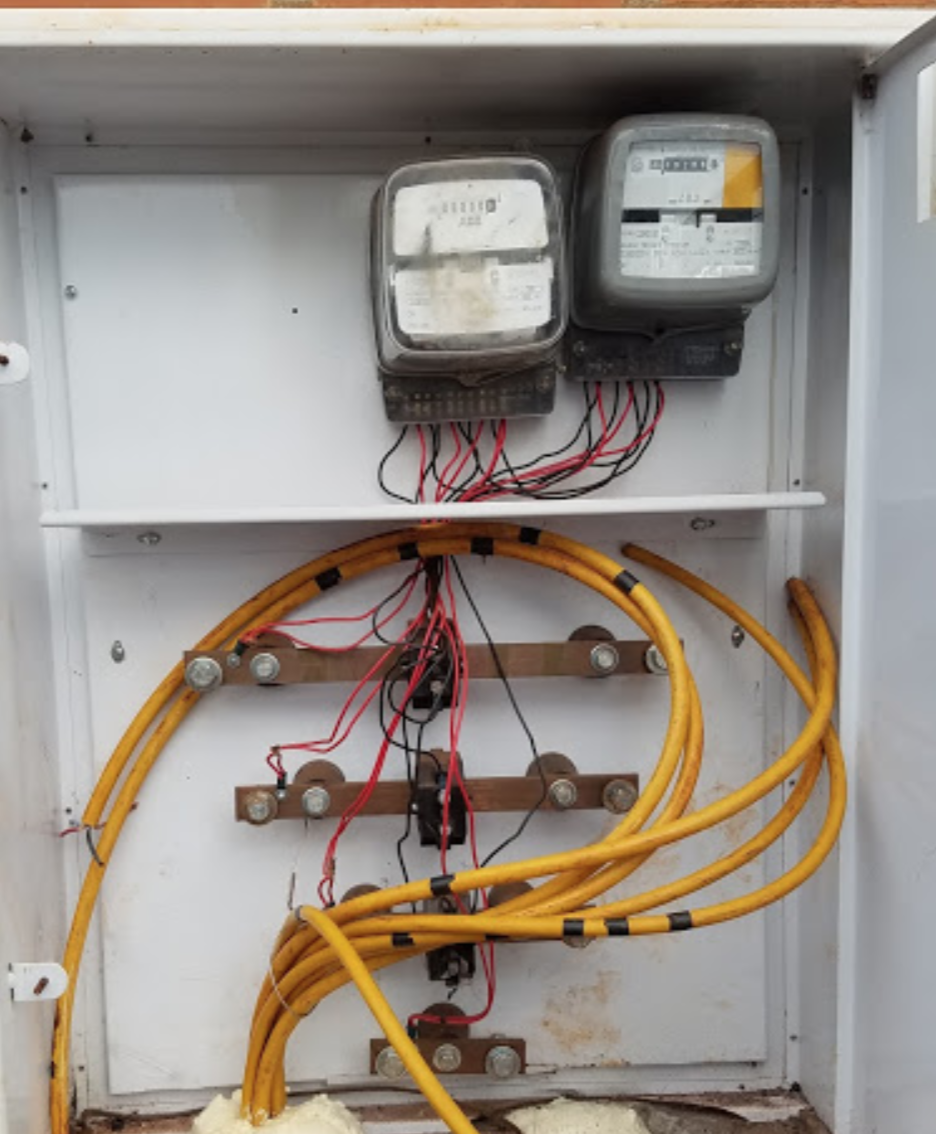
\includegraphics[width=0.5\linewidth]{Figures/Medicion_corriente_con_TI}
	\caption[]{Medición indirecta de corriente empleando transformadores de corriente (TI). Imagen tomada por el autor.}
	\label{fig:medicioncorrienteconti}
\end{figure}
La medición de corriente puede ser directa, vinculando los conductores de alimentación de la carga directamente al medidor o indirecta. Una medición indirecta consiste en reducir los valores de corriente de carga a través de transformadores de corriente (TI) y vincular sus secundarios al medidor \ref{fig:medicioncorrienteconti}. Este último método se emplea en casos donde la corriente calculada supera el valor permitido por el medidor de energía, por lo que será necesario multiplicar el valor de la lectura por un coeficiente correspondiente a la relación de transformación del TI.\\
% TODO: \usepackage{graphicx} required
\begin{figure}
	\centering
	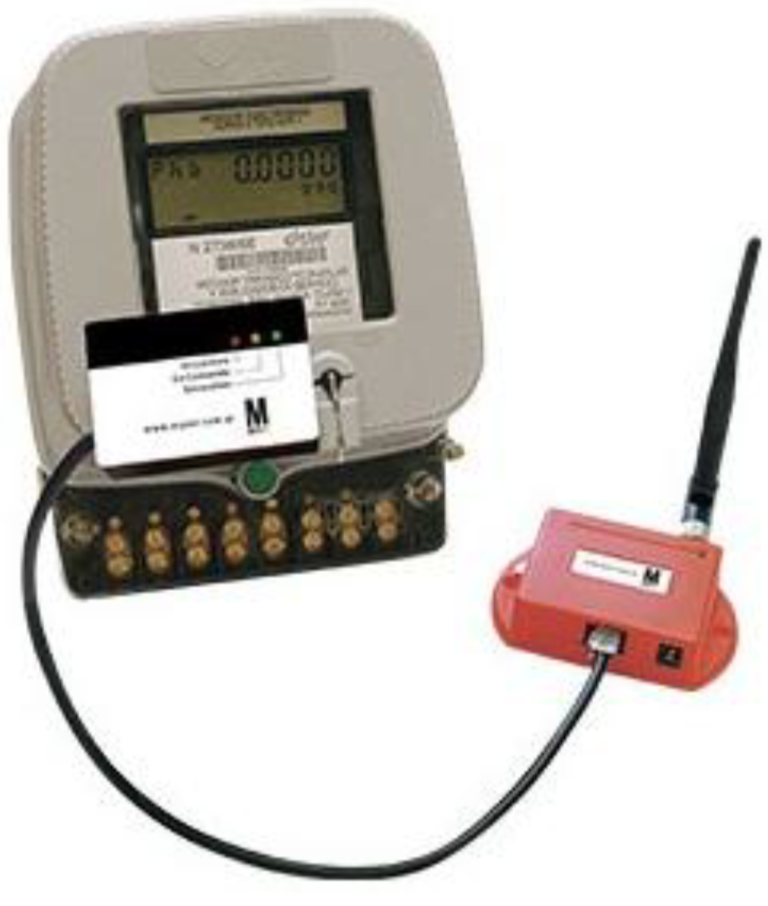
\includegraphics[width=0.5\linewidth]{Figures/medidor_digital_con_complemento_gsm}
	\caption{Medidor de energia digital con complemento para telemedición mediante GSM. Imagen tomada de \citep{MYEEL}}
	\label{fig:medidordigitalconcomplementogsm}
\end{figure}
En la actualidad algunas prestadoras del servicio eléctrico han adoptado estrategias de medición inteligente similares a la presentada en la figura \ref{fig:medidordigitalconcomplementogsm}. En este esquema los equipos de medición se reportan a centros de operación en tiempo semi real a través de una red de comunicaciones movil como por ejemplo GSM.\\
El concepto de telemedición aporta además de lo comercial, valiosa información técnica ya que los centros de operaciones conocen en todo momento el estado del medidor con la posibilidad de detectar fallas o interrupción del servicio eléctrico.\\  
A pesar de tener resultados beneficiosos en lo económico a largo plazo e inmediato en cuanto a calidad del servicio prestado, conlleva una inversión inicial considerable que muchas empresas no están dispuestas a afrontar o no tienen los recursos suficientes para su implementación.\\
\section{Estado del arte y problematica identificada}
En Sudamérica, gran parte de las empresas distibuidoras de energía eléctrica y sus tercerizadas basan parte de sus operaciones en el contacto directo con los usuarios finales mediante reclamos para informarse acerca de interrupciones en el servicio de distribución de energía eléctrica. Una vez recibido un reclamo, la prestadora de servicios envía al grupo de operaciones especializado a recorrer el área circundante al cliente y tratar de determinar el motivo de la interrupción del servicio.\\

% TODO: \usepackage{graphicx} required
\begin{figure}[h!]
	\centering
	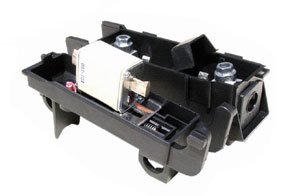
\includegraphics[width=0.7\linewidth]{Figures/NH_aereo_bt}
	\caption{Fusible seccionador aereo tipo NH usualmente utilizado en lineas de distribucion de baja tension}
	\label{fig:nh_aereo_bt}
\end{figure}
Un hecho común en el nordeste Argentino y particularmente en la provincia de Misiones es la destrucción de fusibles aéreos como el presentado en la \ref{fig:nh_aereo_bt}. Estos fusibles conectados inmediatamente a la salida de baja tension y en serie con las líneas de distribución, cumplen la función de protección por sobrecorriente debido a picos de consumo o cortocircuitos causados por desastres naturales como el de la figura \ref{fig:arbolcaidolineabt}. Los fusibles involucrados actúan de manera correcta autodestruyendose e interrumpiendo el paso de corriente.\\
\begin{figure}[h!]
	\centering
	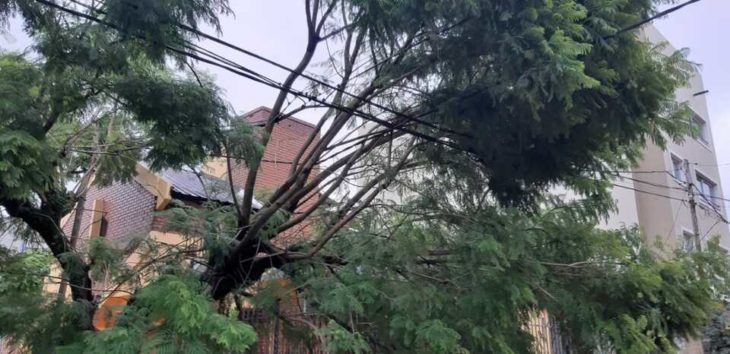
\includegraphics[width=0.7\linewidth]{Figures/arbol_caido_linea_bt}
	\caption{Un árbol caído sobre las líneas de distribución aéreas de baja tensión luego de una breve tormenta en la ciudad de Posadas, Misiones. Imagen tomada de \citep{Noticia_MNES}}
	\label{fig:arbolcaidolineabt}
\end{figure}
Este esquema presentado, resulta aún precario y no efectivo en cuanto a la rapidez para determinar la localización geográfica donde se ha generado una falla, resultando así en una inferior calidad de servicio prestada al cliente.\\

Cabe mencionar que la mayoría de las redes de distribución de baja tensión en 380/220V no poseen la capacidad de brindar algún otro servicio agregado. Algunas redes de media (33 kV) y alta tensión (132 kV) las cuales sin embargo, pueden albergar un conjunto de pelos de fibra óptica (OPGW) los cuales pueden ser utilizados para brindar servicios a terceras partes como empresas de telefonía o bien para monitoreo de la red propiamente dicha. Sin embargo, estas OPGW demuestran cierta vulnerabilidad frente a condiciones climáticas extremas tales como descargas atmosféricas y traen acarreadas un alto costo de mantenimiento \citep{ARTICLE:1}.\\
\citep{ARTICLE:2} y \citep{ARTICLE:3} comparten una arquitectura de 3 capas: física, red y aplicación para sistemas de smart grid. 
A partir del entorno donde residirá la aplicación y su objetivo final, surgen diferentes estrategias de control. Así también, la selección de sensores de diferente tipo tales como meteorológicos e infraestructura \citep{ARTICLE:3} o bien de cargas eléctricas que residen dentro de un entorno controlado haciendo uso de redes de diferente tipo \citep{ARTICLE:2}.\\
Las tecnologías emergentes propias de IoT tales como las redes de comunicación de baja potencia y largo alcance LPWAN \citep{rfc8376}, y las redes tipo malla se analizan y comparan en \citep{ARTICLE:4} como las tecnologías disponibles y viables para dotar de una infraestructura de comunicaciones a las redes de distribución metropolitanas. En \citep{ARTICLE:5} y \citep{Hua} se presentan sistemas de medición de temperatura autónomos utilizando transductores termoeléctricos y electromagnéticos para conversión de energía térmica o electromagnética en energía eléctrica para alimentar la electrónica involucrada y cargar un acumulador.

%----------------------------------------------------------------------------------------

\section{Objetivos y alcance}
\subsection{Objetivo general}
Desarrollar un sistema capaz de determinar valores eficaces de corriente alterna en sistemas metropolitanos de distribución de energía eléctrica en baja tensión y reportar estados a un centro de operaciones a través de una red LoRaWAN de acceso público.\\
\subsection{Objetivos específicos}
\begin{itemize}
	\item Evaluar el uso de un supercapacitor como reemplazo de una batería convencional.\\
	\item Desarrollar una electrónica de ultra bajo consumo para maximizar la autonomía de operación del supercapacitor.
\end{itemize}
\subsection{Alcances}
En el presente documento se desarrollan los siguientes temas:
\begin{itemize}
	\item Circuito de conversión de energía  basado en rectificadores de alta eficiencia.
	\item Acumulador de energía basado en supercapacitores
	\item Patrón de firmware implementado en el microcontrolador para optimizar el uso de energía del acumulador.
	\item Medición de valor RMS de corriente mediante transformador de corriente.
	\item Tecnología LoRaWAN
	\item Recuperación, almacenamiento y presentación de datos generados por los nodos finales.
\end{itemize}
Si bien el proyecto es parte de un plan de una PyME del autor, no  es parte del alcance ni se cubren en este documento las etapa de lanzamiento de producto ni creación de la empresa.
\subsection{Carpetas}

Esta plantilla se distribuye como una único archivo .zip que se puede descomprimir en varios archivos y carpetas. Asimismo, se puede consultar el repositorio git para obtener la última versión de los archivos, \url{https://github.com/patriciobos/Plantilla-CESE.git}. Los nombres de las carpetas son, o pretender ser, auto-explicativos.

\keyword{Appendices} -- Esta es la carpeta donde se deben poner los apéndices. Cada apéndice debe ir en su propio archivo \file{.tex}. Se incluye un ejemplo y una plantilla en la carpeta.

\keyword{Chapters} -- Esta es la carpeta donde se deben poner los capítulos de la memoria. Cada capítulo debe ir un su propio archivo \file{.tex} por separado.  Se ofrece por defecto, la siguiente estructura de capítulos y se recomienda su utilización dentro de lo posible:

\begin{itemize}
\item Capítulo 1: Introducción general	
\item Capítulo 2: Introducción específica
\item Capítulo 3: Diseño e implementación
\item Capítulo 4: Ensayos y resultados
\item Capítulo 5: Conclusiones

\end{itemize}

Esta estructura de capítulos es la que se recomienda para las memorias de la especialización.

\keyword{Figures} -- Esta carpeta contiene todas las figuras de la memoria.  Estas son las versiones finales de las imágenes que van a ser incluidas en la memoria.  Pueden ser imágenes en formato \textit{raster}\footnote{\url{https://en.wikipedia.org/wiki/Raster_graphics}} como \file{.png}, \file{.jpg} o en formato vectoriales\footnote{\url{https://en.wikipedia.org/wiki/Vector_graphics}} como \file{.pdf}, \file{.ps}.  Se debe notar que utilizar imágenes vectoriales disminuye notablemente el peso del documento final y acelera el tiempo de compilación por lo que es recomendable su utilización siempre que sea posible.

\subsection{Archivos}

También están incluidos varios archivos, la mayoría de ellos son de texto plano y se puede ver su contenido en un editor de texto. Después de la compilación inicial, se verá que más archivos auxiliares son creados por \ LaTeX{} o BibTeX, pero son de uso interno y no es necesario hacer nada en particular con ellos.  Toda la información necesaria para compilar el documento se encuentra en los archivos \file{.tex}, \file{.bib}, \file{.cls} y en las imágenes de la carpeta Figures.

\keyword{referencias.bib} - este es un archivo importante que contiene toda la información de referencias bibliográficas que se utilizarán para las citas en la memoria en conjunto con BibTeX. Usted puede escribir las entradas bibliográficas en forma manual, aunque existen también programas de gestión de referencias que facilitan la creación y gestión de las referencias y permiten exportarlas en formato BibTeX.  También hay disponibles sitios web como \url{books.google.com} que permiten obtener toda la información necesaria para una cita en formato BibTeX. Ver sección \ref{sec:biblio}

\keyword{MastersDoctoralThesis.cls} -- este es un archivo importante. Es el archivos con la clase que le informa a \LaTeX{} cómo debe dar formato a la memoria. El usuario de la plantilla no debería necesitar modificar nada de este archivo.

\keyword{memoria.pdf} -- esta es su memoria con una tipografía bellamente compuesta (en formato de archivo PDF) creado por \LaTeX{}. Se distribuye con la plantilla y después de compilar por primera vez sin hacer ningún cambio se debería obtener una versión idéntica a este documento.

\keyword{memoria.tex} -- este es un archivo importante. Este es el archivo que tiene que compilar \LaTeX{} para producir la memoria como un archivo PDF. Contiene un marco de trabajo y estructuras que le indican a \LaTeX{} cómo diagramar la memoria.  Está altamente comentado para que se pueda entender qué es lo que realiza cada línea de código y por qué está incluida en ese lugar.  En este archivo se debe completar la información personalizada de las primeras sección según se indica en la sección \ref{sec:FillingFile}.

Archivos que \emph{no} forman parte de la distribución de la plantilla pero que son generados por \LaTeX{} como archivos auxiliares necesarios para la producción de la memoria.pdf son:

\keyword{memoria.aux} -- este es un archivo auxiliar generado por \LaTeX{}, si se borra \LaTeX{} simplemente lo regenera cuando se compila el archivo principal \file{memoria.tex}.

\keyword{memoria.bbl} -- este es un archivo auxiliar generado por BibTeX, si se borra BibTeX simplemente lo regenera cuando se compila el archivo principal \file{memoria.tex}. Mientras que el archivo \file{.bib} contiene todas las referencias que hay, este archivo \file{.bbl} contine sólo las referencias que han sido citadas y se utiliza para la construcción de la bibiografía.

\keyword{memoria.blg} -- este es un archivo auxiliar generado por BibTeX, si se borra BibTeX simplemente lo regenera cuando se compila el archivo principal \file{memoria.tex}.

\keyword{memoria.lof} -- este es un archivo auxiliar generado por \LaTeX{}, si se borra \LaTeX{} simplemente lo regenera cuando se compila el archivo principal \file{memoria.tex}.  Le indica a \LaTeX{} cómo construir la sección \emph{Lista de Figuras}.
 
\keyword{memoria.log} --  este es un archivo auxiliar generado por \LaTeX{}, si se borra \LaTeX{} simplemente lo regenera cuando se compila el archivo principal \file{memoria.tex}. Contiene mensajes de \LaTeX{}. Si se reciben errores o advertencias durante la compilación, se guardan en este archivo \file{.log}.

\keyword{memoria.lot} -- este es un archivo auxiliar generado por \LaTeX{}, si se borra \LaTeX{} simplemente lo regenera cuando se compila el archivo principal \file{memoria.tex}.  Le indica a \LaTeX{} cómo construir la sección \emph{Lista de Tablas}.

\keyword{memoria.out} -- este es un archivo auxiliar generado por \LaTeX{}, si se borra \LaTeX{} simplemente lo regenera cuando se compila el archivo principal \file{memoria.tex}.

De esta larga lista de archivos, sólo aquellos con la extensión \file{.bib}, \file{.cls} y \file{.tex} son importantes.  Los otros archivos auxiliares pueden ser ignorados o borrados ya que \LaTeX{} y BibTeX los regenerarán durante la compilación.

%----------------------------------------------------------------------------------------

\section{Entorno de trabajo}

Ante de comenzar a editar la plantilla debemos tener un editor \LaTeX{} instalado en nuestra computadora.  En forma análoga a lo que sucede en lenguaje C, que se puede crear y editar código con casi cualquier editor, existen ciertos entornos de trabajo que nos pueden simplificar mucho la tarea.  En este sentido, se recomienda, sobre todo para los principiantes en \LaTeX{} la utilización de TexMaker, un programa gratuito y multi-plantaforma que está disponible tanto para windows como para sistemas GNU/linux.

La versión más reciente de TexMaker es la 4.5 y se puede descargar del siguiente link: \url{http://www.xm1math.net/texmaker/download.html}. Se puede consultar el manual de usuario en el siguiente link: \url{http://www.xm1math.net/texmaker/doc.html}.
 

\subsection{Paquetes adicionales}

Si bien durante el proceso de instalación de TexMaker, o cualquier otro editor que se haya elegido, se instalarán en el sistema los paquetes básicos necesarios para trabajar con \LaTeX{}, la plantilla de los trabajos de Especialización y Maestría requieren de paquete adicionales.

Se indican a continuación los comandos que se deben introducir en la consola de Ubuntu (ctrl + alt + t) para instalarlos:

\begin{lstlisting}[language=bash]
  $ sudo apt install texlive-lang-spanish texlive-science 
  $ sudo apt install texlive-bibtex-extra biber
  $ sudo apt install texlive texlive-fonts-recommended
  $ sudo apt install texlive-latex-extra
\end{lstlisting}


\subsection{Configurando TexMaker}


Una vez instalado el programa y los paquetes adicionales se debe abrir el archivo memoria.tex con el editor para ver una pantalla similar a la que se puede apreciar en la figura \ref{fig:texmaker}. 

\begin{figure}[h]
	\centering
	\includegraphics[width=\textwidth]{./Figures/texmaker.png}
	\caption{Entorno de trabajo de texMaker.}
	\label{fig:texmaker}
\end{figure}

Notar que existe una vista llamada Estructura a la izquierda de la interfaz que nos permite abrir desde dentro del programa los archivos individuales de los capítulos.  A la derecha se encuentra una vista con el archivo propiamente dicho para su edición. Hacia la parte inferior se encuentra una vista del log con información de los resultados de la compilación.  En esta última vista pueden aparecen advertencias o \textit{warning}, que normalmente pueden ser ignorados, y los errores que se indican en color rojo y deben resolverse para que se genere el PDF de salida.

Recordar que el archivo que se debe compilar con PDFLaTeX es \file{memoria.tex}, si se tratara de compilar alguno de los capítulos saldría un error.  Para salvar la molestia de tener que cambiar de archivo para compilar cada vez que se realice una modificación en un capítulo, se puede definir el archivo \file{memoria.tex} como ``documento maestro'' yendo al menú opciones -> ``definir documento actual como documento maestro'', lo que permite compilar con PDFLaTeX memoria.tex directamente desde cualquier archivo que se esté modificando . Se muestra esta opción en la figura \ref{fig:docMaestro}.

\begin{figure}[h]
	\centering
	\includegraphics[width=\textwidth]{./Figures/docMaestro.png}
	\caption{Definir memoria.tex como documento maestro.}
	\label{fig:docMaestro}
\end{figure}

En el menú herramientas se encuentran las opciones de compilación.  Para producir un archivo PDF a partir de un archivo .tex se debe ejecutar PDFLaTeX (el shortcut es F6). Para incorporar nueva bibliografía se debe utilizar la opción BibTeX del mismo menú herramientas (el shortcut es F11).

Notar que para actualizar las tablas de contenidos se debe ejecutar PDFLaTeX dos veces.  Esto se debe a que es necesario actualizar algunos archivos auxiliares antes de obtener el resultado final.  En forma similar, para actualizar las referencias se debe ejecutar primero PDFLaTeX, después BibTeX y finalmente PDFLaTeX dos veces por idénticos motivos.

\section{Personalizando la plantilla, el archivo \file{memoria.tex}}
\label{sec:FillingFile}

Para personalizar la plantilla se debe incorporar la información propia en los distintos archivos \file{.tex}. 

Primero abrir \file{memoria.tex} con TexMaker (o el editor de su preferencia). Se debe ubicar dentro del archivo el bloque de código titulado \emph{INFORMACIÓN DE LA PORTADA} donde se deben incorporar los primeros datos personales con los que se construirá automáticamente la portada.


%----------------------------------------------------------------------------------------

\section{El código del archivo \file{memoria.tex} explicado}

El archivo \file{memoria.tex} contiene la estructura del documento y es el archivo de mayor jerarquía de la memoria.  Podría ser equiparable a la función \emph{main()} de un programa en C, o mejor dicho al archivo fuente .c donde se encuentra definida la función main().

La estructura básica de cualquier documento de \LaTeX{} comienza con la definición de clase del documento, es seguida por un preámbulo donde se pueden agregar funcionalidades con el uso de \texttt{paquetes} (equiparables a bibliotecas de C), y finalmente, termina con el cuerpo del documento, donde irá el contenido de la memoria.

\lstset{%
  basicstyle=\small\ttfamily,
  language=[LaTeX]{TeX}
}

\begin{lstlisting}
\documentclass{article}  <- Definicion de clase
\usepackage{listings}	 <- Preambulo

\begin{document}	 <- Comienzo del contenido propio 
	Hello world!
\end{document}
\end{lstlisting}


El archivo \file{memoria.tex} se encuentra densamente comentado para explicar qué páginas, secciones y elementos de formato está creando el código \LaTeX{} en cada línea. El código está dividido en bloques con nombres en mayúsculas para que resulte evidente qué es lo que hace esa porción de código en particular. Inicialmente puede parecer que hay mucho código \LaTeX{}, pero es principalmente código para dar formato a la memoria por lo que no requiere intervención del usuario de la plantilla.  Sí se deben personalizar con su información los bloques indicados como:

\begin{itemize}
	\item Informacion de la memoria
	\item Resumen
	\item Agradecimientos
	\item Dedicatoria
\end{itemize}

El índice de contenidos, las listas de figura de tablas se generan en forma automática y no requieren intervención ni edición manual por parte del usuario de la plantilla. 

En la parte final del documento se encuentran los capítulos y los apéndices.  Por defecto se incluyen los 5 capítulos propuestos que se encuentran en la carpeta /Chapters. Cada capítulo se debe escribir en un archivo .tex separado y se debe poner en la carpeta \emph{Chapters} con el nombre \file{Chapter1}, \file{Chapter2}, etc\ldots El código para incluir capítulos desde archivos externos se muestra a continuación.

\begin{verbatim}
	\include{Chapters/Chapter1}
	\include{Chapters/Chapter2} 
	\include{Chapters/Chapter3}
	\include{Chapters/Chapter4} 
	\include{Chapters/Chapter5} 
\end{verbatim}

Los apéndices también deben escribirse en archivos .tex separados, que se deben ubicar dentro de la carpeta \emph{Appendices}. Los apéndices vienen comentados por defecto con el caracter \code{\%} y para incluirlos simplemente se debe eliminar dicho caracter.

Finalmente, se encuentra el código para incluir la bibliografía en el documento final.  Este código tampoco debe modificarse. La metodología para trabajar las referencias bibliográficas se desarrolla en la sección \ref{sec:biblio}.
%----------------------------------------------------------------------------------------

\section{Bibliografía}
\label{sec:biblio}

Las opciones de formato de la bibliografía se controlan a través del paquete de latex \option{biblatex} que se incluye en la memoria en el archivo memoria.tex.  Estas opciones determinan cómo se generan las citas bibliográficas en el cuerpo del documento y cómo se genera la bibliografía al final de la memoria.

En el preámbulo se puede encontrar el código que incluye el paquete biblatex, que no requiere ninguna modificación del usuario de la plantilla, y que contiene las siguientes opciones:

\begin{lstlisting}
\usepackage[backend=bibtex,
	natbib=true, 
	style=numeric, 
	sorting=none]
{biblatex}
\end{lstlisting}

En el archivo \file{reference.bib} se encuentran las referencias bibliográficas que se pueden citar en el documento.  Para incorporar una nueva cita al documento lo primero es agregarla en este archivo con todos los campos necesario.  Todas las entradas bibliográficas comienzan con $@$ y una palabra que define el formato de la entrada.  Para cada formato existen campos obligatorios que deben completarse. No importa el orden en que las entradas estén definidas en el archivo .bib.  Tampoco es importante el orden en que estén definidos los campos de una entrada bibliográfica. A continuación se muestran algunos ejemplos:

\begin{lstlisting}
@ARTICLE{ARTICLE:1,
    AUTHOR="John Doe",
    TITLE="Title",
    JOURNAL="Journal",
    YEAR="2017",
}
\end{lstlisting}


\begin{lstlisting}
@BOOK{BOOK:1,
    AUTHOR="John Doe",
    TITLE="The Book without Title",
    PUBLISHER="Dummy Publisher",
    YEAR="2100",
}
\end{lstlisting}


\begin{lstlisting}
@INBOOK{BOOK:2,
    AUTHOR="John Doe",
    TITLE="The Book without Title",
    PUBLISHER="Dummy Publisher",
    YEAR="2100",
    PAGES="100-200",
}
\end{lstlisting}


\begin{lstlisting}
@MISC{WEBSITE:1,
    HOWPUBLISHED = "\url{http://example.com}",
    AUTHOR = "Intel",
    TITLE = "Example Website",
    MONTH = "12",
    YEAR = "1988",
    URLDATE = {2012-11-26}
}
\end{lstlisting}

Se debe notar que los nombres \emph{ARTICLE:1}, \emph{BOOK:1}, \emph{BOOK:2} y \emph{WEBSITE:1} son nombres de fantasía que le sirve al autor del documento para identificar la entrada. En este sentido, se podrían reemplazar por cualquier otro nombre.  Tampoco es necesario poner : seguido de un número, en los ejemplos sólo se incluye como un posible estilo para identificar las entradas.

La entradas se citan en el documento con el comando: 

\begin{verbatim}
\citep{nombre_de_la_entrada}
\end{verbatim}

Y cuando se usan, se muestran así: \citep{ARTICLE:1}, \citep{BOOK:1}, \citep{BOOK:2}, \citep{WEBSITE:1}.  Notar cómo se conforma la sección Bibliografía al final del documento. 

	\chapter{Introducción específica} % Main chapter title
\label{Chapter2}
%----------------------------------------------------------------------------------------
%	SECTION 1
%----------------------------------------------------------------------------------------
En este capítulo se presentan los requerimientos acordados con el cliente y los recursos de \textit{hardware} (HW) y \textit{software} (SW) utilizados para el desarrollo del trabajo. Se describen en las partes implementadas del HW, los servicios integrados de \textit{backend} (BES) y solamente algunos aspectos relevantes del \textit{firmware} (FW) que interactúa con el HW. En el capítulo 3 se abarca la lógica de negocios implementada en el FW del microcontrolador.\\
\section{Requerimientos acordados con el cliente}
\label{sec:requerimientos}
\begin{enumerate}
	\item Grupo de requerimientos asociados con hardware
	\begin{enumerate}
		\item El dispositivo deberá ser de tipo \textit{plug and play}.
		\item El circuito impreso no deberá ocupar un volumen mayor a 10x10x5 cm.
		\item Basarse en un microcontrolador ESP32 y disponer de:
		\begin{enumerate}%[label*=\arabic*.]
			\item 4 entradas analógicas.
			\item 3 salidas digitales.
			\item Unidad UART.
			\item Integrar un módulo de comunicaciones LoRa.
		\end{enumerate}
		\item Deberá tener al menos 12 horas de autonomía de funcionamiento.
		\item Bajo consumo en modo ocioso: el consumo del hardware en total, no deberá superar los 5 mA cuando no está midiendo ni transmitiendo.
		\item El circuito elevador de tensión DC-DC deberá:
		\begin{enumerate}%[label*=\arabic*.]
			\item Funcionar con tensiones menores a 2V en la entrada.
			\item Otorgar 5 Volts a la salida.
			\item Ser capaz de otorgar 300 miliamperes a la salida.
		\end{enumerate}
		\item El transformador de corriente (TI) debe:
		\begin{enumerate}%[label*=\arabic*.]
			\item Ser de tipo núcleo partido.
			\item Admitir 100 Amperes de corriente en el circuito primario y un máximo 5 Amperes en el circuito secundario.
		\end{enumerate}
		\item \label{req_relay} El relay encargado de cambiar el modo de operación debe:
		\begin{enumerate}%[label*=\arabic*.]
			\item Ser de tipo doble inversor sin retención.
			\item Su bobina debe poder energizarse con 5V o menos.
			\item Soportar al menos 5 Amperes de corriente por los contactos.
		\end{enumerate} 
		\item Debe funcionar de manera independiente a la frecuencia de operación de la red 50/60 Hz.
		\item Debe funcionar de manera independiente a la tensión de fase del sistema de distribución 110/220 Voltios.
	\end{enumerate}
	\item Grupo de requerimientos asociados con el firmware
	\begin{enumerate}
		\item Debe manejar un módulo de comunicación LoRa y protocolo LoRaWAN.
		\item Deberá tener un porcentaje de cobertura de tests unitarios del 60\% como mínimo.
		\item Antes configurarse en modo ocioso, debe desenergizar la etapa de medición de corriente y el módulo de comunicaciones con el objeto de ahorrar energía.
	\end{enumerate}
	
	\item Grupo de requerimientos asociados con los servicios de backend (BES)
	\label{requerimientos_backend}
	\begin{enumerate}
		\item Todos los servicios deben poder correr en una Raspberry Pi 3.
		\item El \textit{software} de los BES se desarrollará en lenguaje Python.
		\item Recuperar los datos de la red LoRaWAN.\label{requerimiento_LORAWAN}
		\item Almacenar los datos en una tabla de MySQL.
		\item (GUI - \textit{Graphical User Interface}) basada en Grafana.
	\end{enumerate}
	
	\item Grupo de requerimientos asociados con ensayos de integración y \textit{end-to-end}
	\begin{enumerate}
		\item El banco de ensayos de \textit{hardware} debe contar con una carga fantasma de al menos 10 Amperes y permitir realizar interrupciones de corriente de manera programada mediante una computadora adicional tipo Raspberry Pi o de manera manual.
		\item Los BES deben estar operativos al momento de realizar los ensayos.
		\item Contar con un gateway de acceso a una red LoRaWAN como por ejemplo \textit{The Things Network}.
	\end{enumerate}
\end{enumerate}


\section{Diagrama de bloques general del sistema implementado}
El diagrama de bloques del HW a instalar \textit{in situ} es presentado en la figura \ref{fig:diagramadebloquesdelhw} y consta de cuatro bloques:
% TODO: \usepackage{graphicx} required
\begin{figure}[h!]
	\centering
	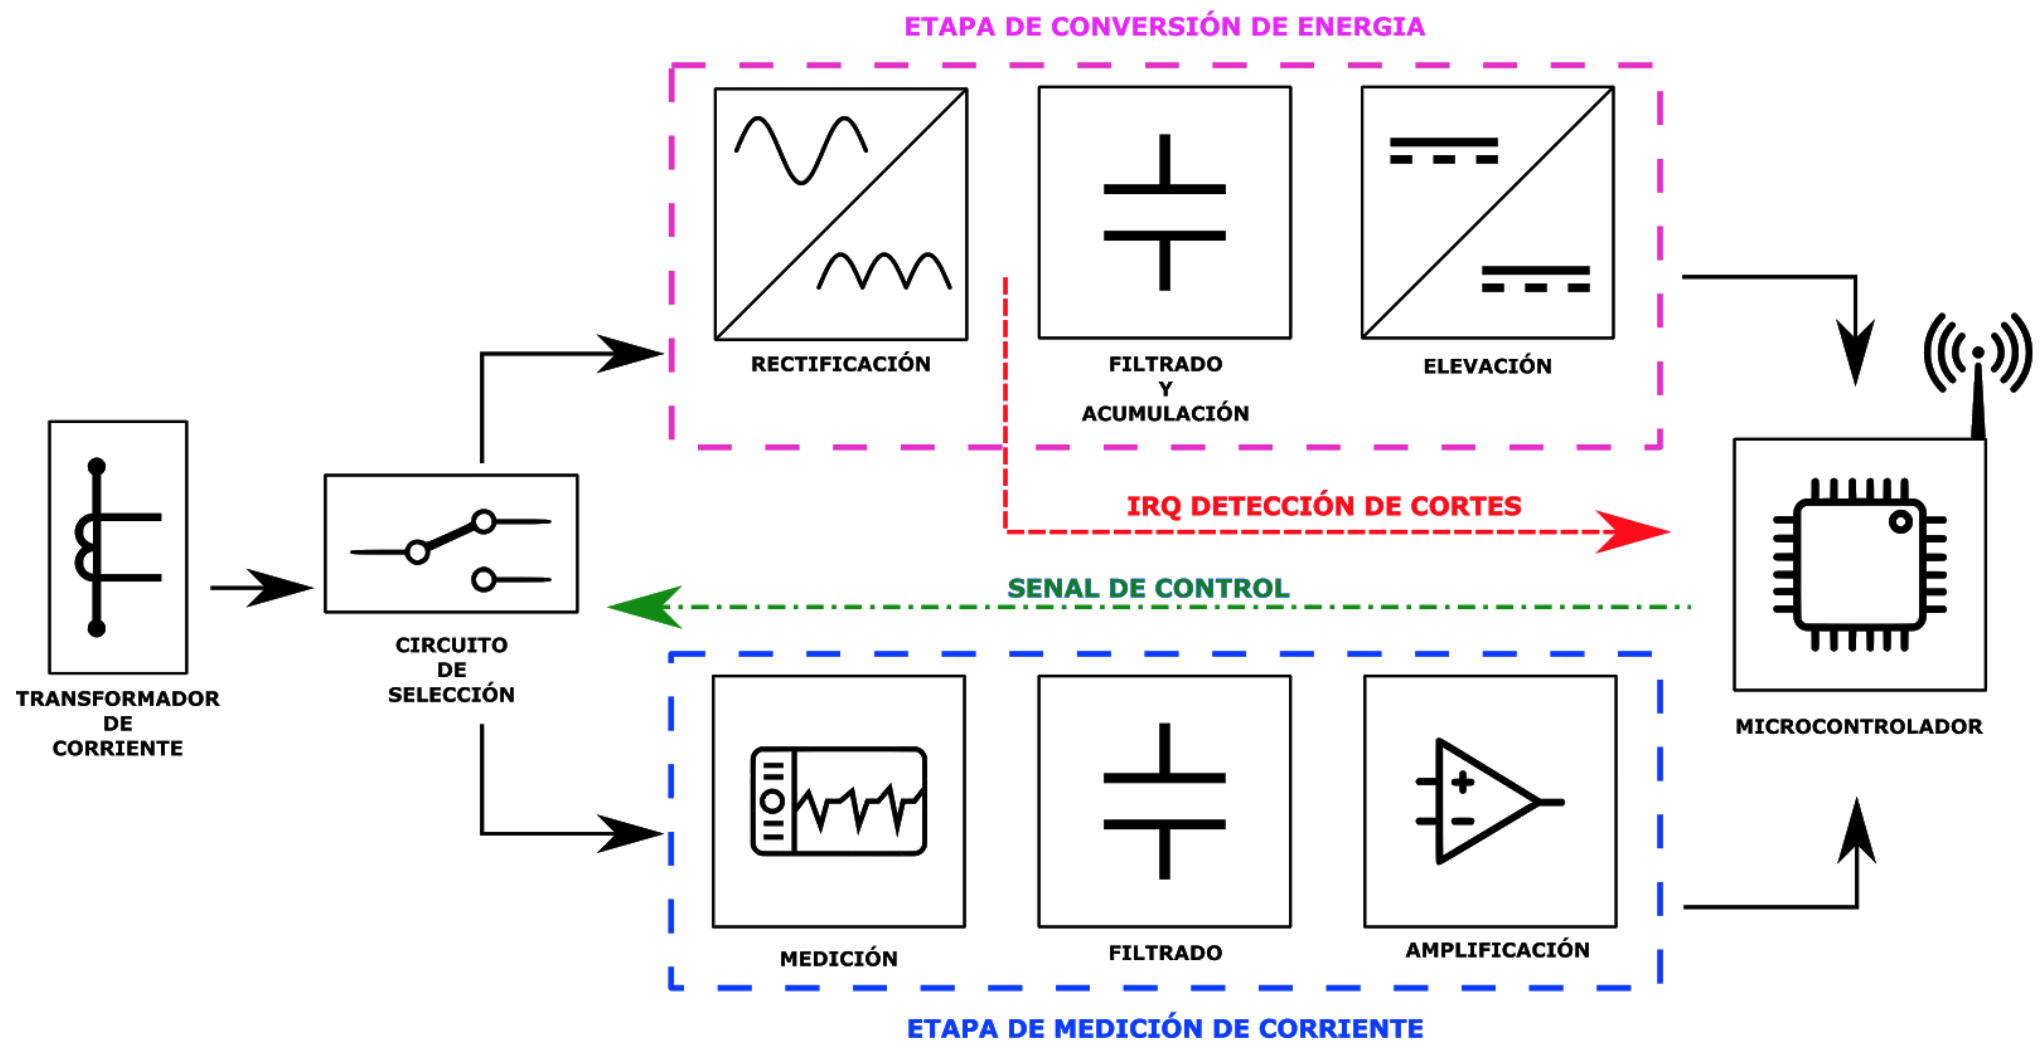
\includegraphics[width=0.7\linewidth]{Figures/diagrama_de_bloques_del_HW}
	\caption{Diagrama de bloques del HW para el nodo a instalar \textit{in situ}}
	\label{fig:diagramadebloquesdelhw}
\end{figure}
\begin{enumerate}
	\item Circuito de selección de modo: un relay (RL) y su circuito de mando controlarán a que etapa del nodo se conectarán los terminales del TI.
	\item Etapa de rectificación, acumulación de energía y elevación de tensión: compuesta por rectificador de onda completa, una etapa de filtrado y acumulación y un circuito elevador de tensión.
	\item Etapa de medición de valor RMS de corriente: un chip dedicado toma la señal de tensión generada en bornes del resistor shunt y calcula el valor RMS. A su salida entrega un valor proporcional de tensión DC.
	\item Microcontrolador (MC): ejecuta la lógica de negocios que rige el comportamiento del nodo, digitalizar mediciones y transmitir datos a la red LoRaWAN.
\end{enumerate}
Por otro lado, el sistema también implicó el desarrollo y puesta en funcionamiento de un conjunto de servicios de \textit{backend} (BES) propios del proyecto que cumplen las funciones de:
\begin{itemize}
	\item Recuperación de datos de la red LoRaWAN.
	\item Almacenamiento en una base de datos (DB).
	\item Presentación de los datos al usuario final mediante una interfaz gráfica de usuario (GUI).
\end{itemize}

El requisito \ref{requerimiento_LORAWAN} impuso el uso de una red LoRaWAN como columna vertebral para la transmisión de datos generados por los nodos. Para cumplirlo se adoptó la arquitectura presentada en la figura \ref{fig:diagramadebloquesdebes}.\\
% TODO: \usepackage{graphicx} required
\begin{figure}[h!]
	\centering
	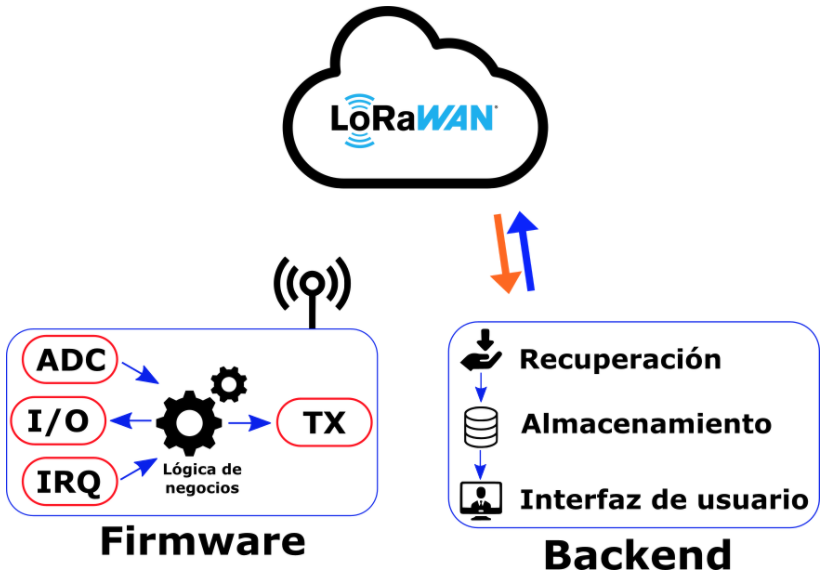
\includegraphics[width=0.6\linewidth]{Figures/diagrama_de_bloques_de_BES}
	\caption{Diagrama de bloques del FW implementado en el MC y su interacción con la red LoRaWAN y los BES privados del sistema.}
	\label{fig:diagramadebloquesdebes}
\end{figure}\\
Las mediciones son tomadas por el HW y transmitidas hacia la red LoRaWAN para luego interactuar con los BES privados que se encargan de recuperar, almacenar y presentar los datos al usuario final.\\


\section{Detalle del hardware}
\subsection{Transformador de corriente}
Un transformador de corriente o intensidad (TI) es un dispositivo de medición utilizado para producir en su devanado secundario una corriente diferente y proporcional a la que circula por su devanado primario.\\
El principio de operación de un TI no es diferente al de un transformador de potencia convencional. A diferencia de uno de potencia, el devanado primario puede ser de una sola vuelta sobre un núcleo ferromagnético como se ve en la figura \ref{fig:dibujomedicionti}. El devanado secundario suele tener un número mayor de vueltas alrededor del núcleo y depende de que tanto se debe reducir la corriente.\\
% TODO: \usepackage{graphicx} required
\begin{figure}[h!]
	\centering
	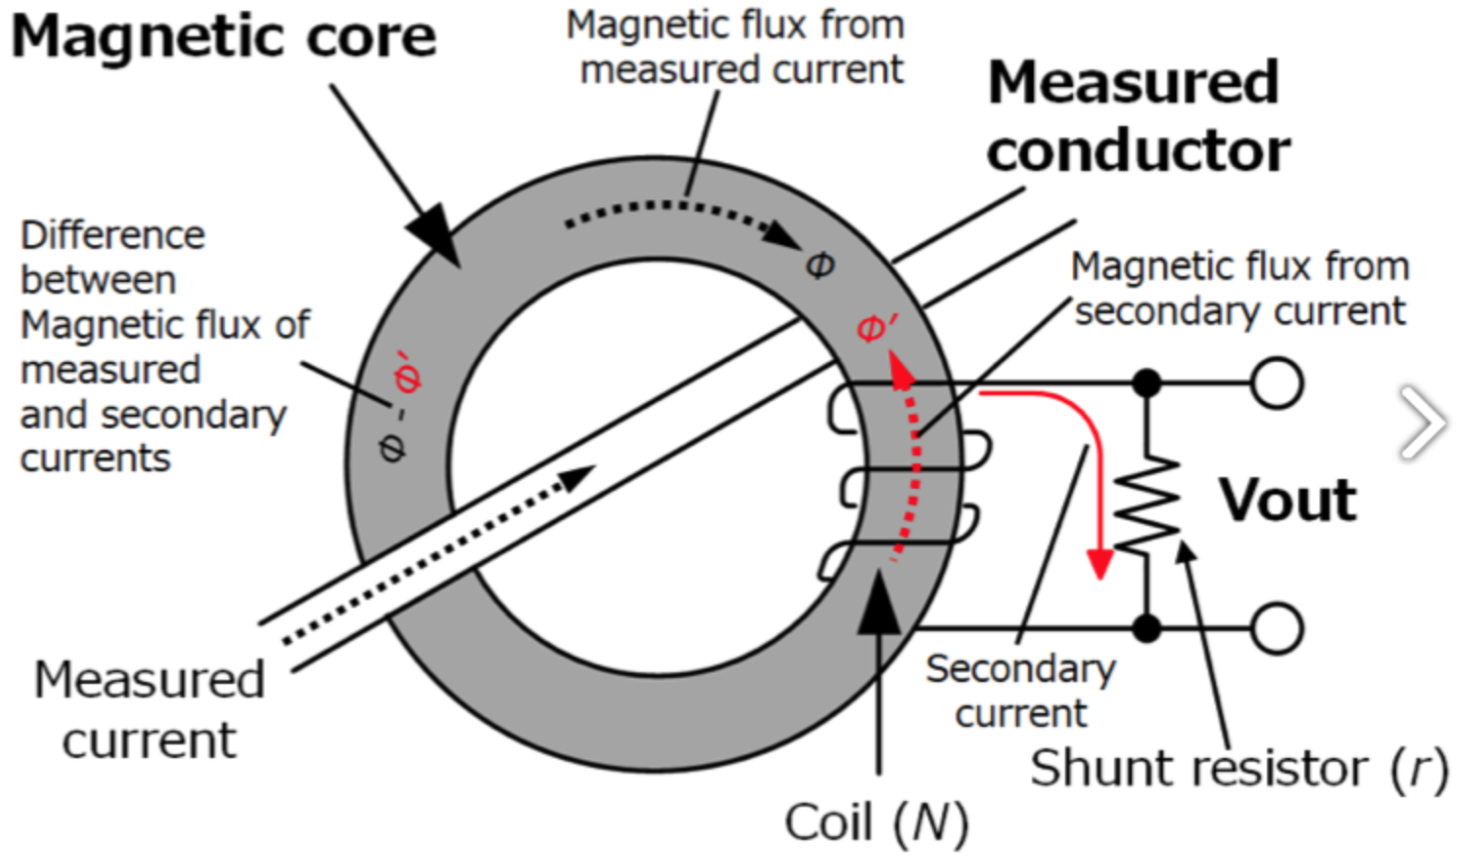
\includegraphics[width=0.5\linewidth]{Figures/dibujo_medicion_TI}
	\caption{Circuito de medición indirecta de corriente mediante un TI.\citep{hioki}}
	\label{fig:dibujomedicionti}
\end{figure}\\
Muchos TI tienen una relación estándar de 5 Amperes en el secundario, por ejemplo un TI 200/5 significa que cuando por el primario fluyen 200 amperes en el secundario solo fluyen 5. Es decir, el TI tiene una relación de transformación de corriente N de 40 veces.\\
Mediante esta técnica, pequeños instrumentos pueden monitorear grandes valores de corriente manteniendo una distancia segura de las líneas de alta tensión.


\subsection{Circuito de selección}
A partir del lineamiento de que el TI debe estar conectado por defecto a la entrada del rectificador y al resistor shunt al energizarse la bobina del RL, el número y la disposición de los contactos fue un factor relevante al momento de elegir la mejor opción. La variante comercial que cumplió con los requisitos \ref{req_relay} es la producida por la firma Hongfa modelo HF115F/005-2ZS4A presentada en la figura \ref{fig:relay}.
\begin{figure}[h!]
    \centering
	\begin{subfigure}[b]{0.3\textwidth}
		\centering
		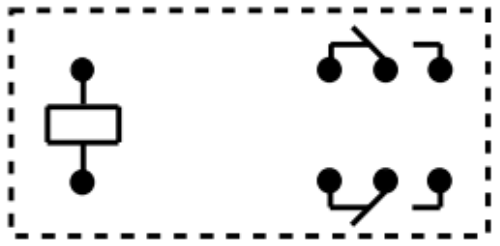
\includegraphics[width=.65\textwidth]{./Figures/relay_pinout}
		\caption{}
		\label{fig:relay_pinout}
	\end{subfigure}
    \centering
	\begin{subfigure}[b]{0.3\textwidth}
		\centering
		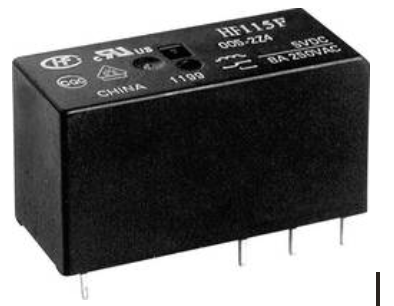
\includegraphics[width=.65\textwidth]{./Figures/relay_encapsulado}
		\caption{}
		\label{fig:relay_encapsulado}
	\end{subfigure}
	\caption{Pinout del relay HF115F/005-2ZS4A (izquireda) y su encapsulado (derecha). Imágenes tomadas de \citep{datasheet_relay}}
	\label{fig:relay}
\end{figure}

\subsection{Conversión de energía}
Para obtener una tensión continua a partir de una alterna generada por el TI, es necesario implementar un puente rectificador de onda completa.\\
En la actualidad la mayoría de los circuitos rectificadores de onda completa se basan en diodos de silicio de bajo costo. Sin embargo, un diodo de silicio posee una caída de tensión típica de 0,7 V. Esta caída de tensión se traduce en pérdidas por efecto Joule y es relevante en dispositivos donde la conversión, acumulación y gestión de energía es crítica. Por lo tanto, se desea maximizar la transferencia de tensión y potencia entre entrada y salida del puente rectificador.\\
Yilmaz \citep{Yilmaz} analiza técnicas de rectificación de onda completa con diferentes tipos de diodos, como así también un arreglo de transistores MOSFET pasivo y activo. Las caídas de tensión simuladas entre la entrada y salida entre un puente rectificador de diodos de silicio y uno pasivo basado en MOSFETs se comparan en la figura \ref{fig:comparacion_diodos_vs_MOSFET}.\\

\begin{figure}[h!]
	\begin{subfigure}{.5\textwidth}
		\centering
		% include first image
		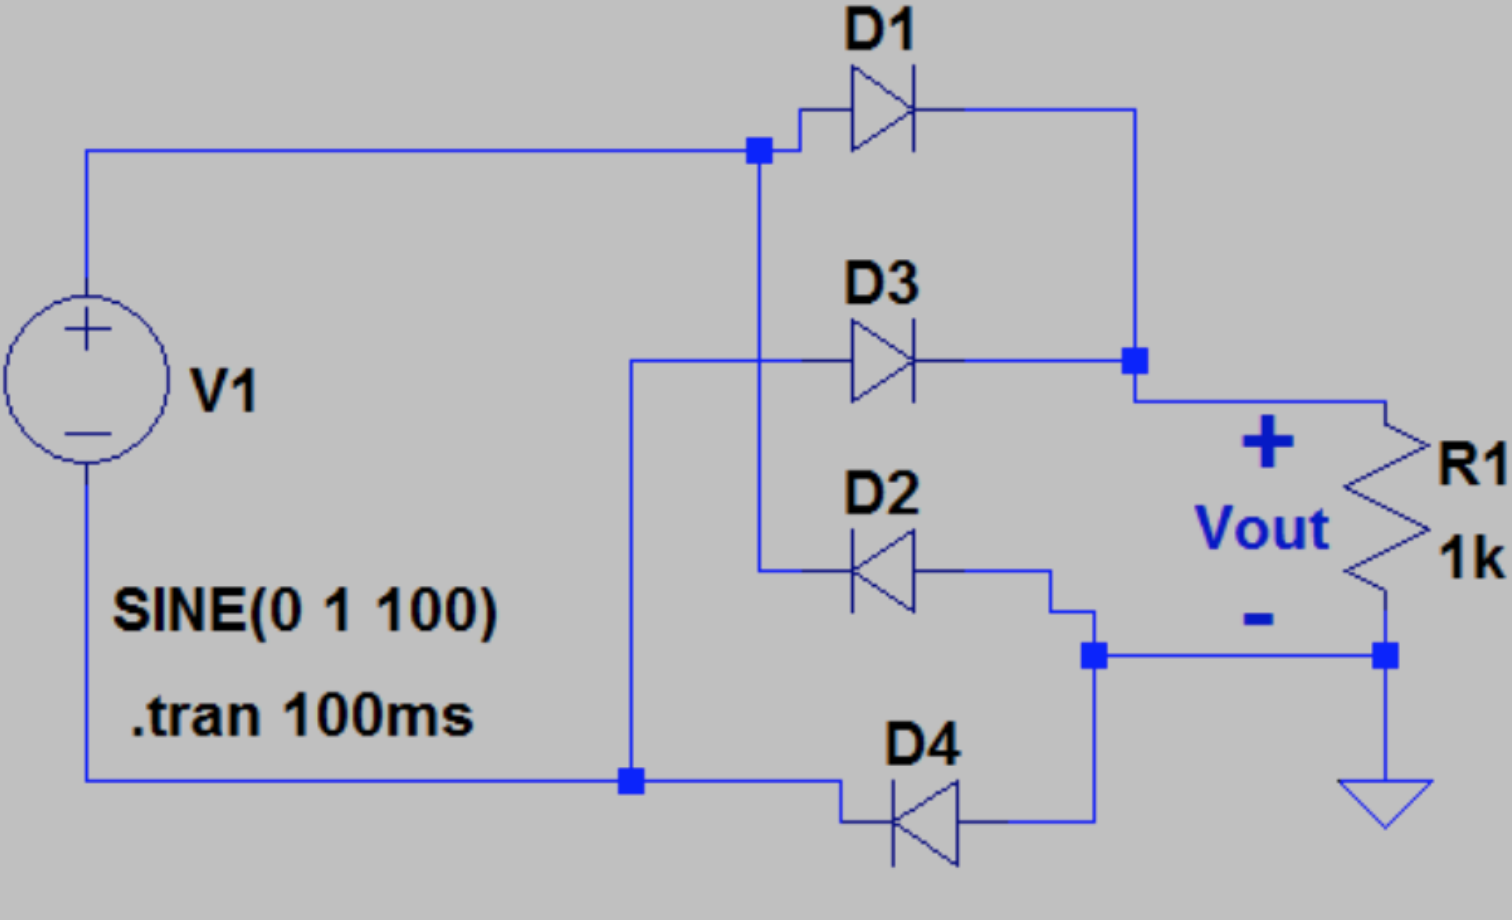
\includegraphics[width=.8\linewidth]{Figures/YILMAZ_silicon_diode_rectifier}  
		\caption{Rectificador basado en diodos de silicio}
		\label{fig:rect_diodos}
	\end{subfigure}
	\begin{subfigure}{.5\textwidth}
		\centering
		% include second image
		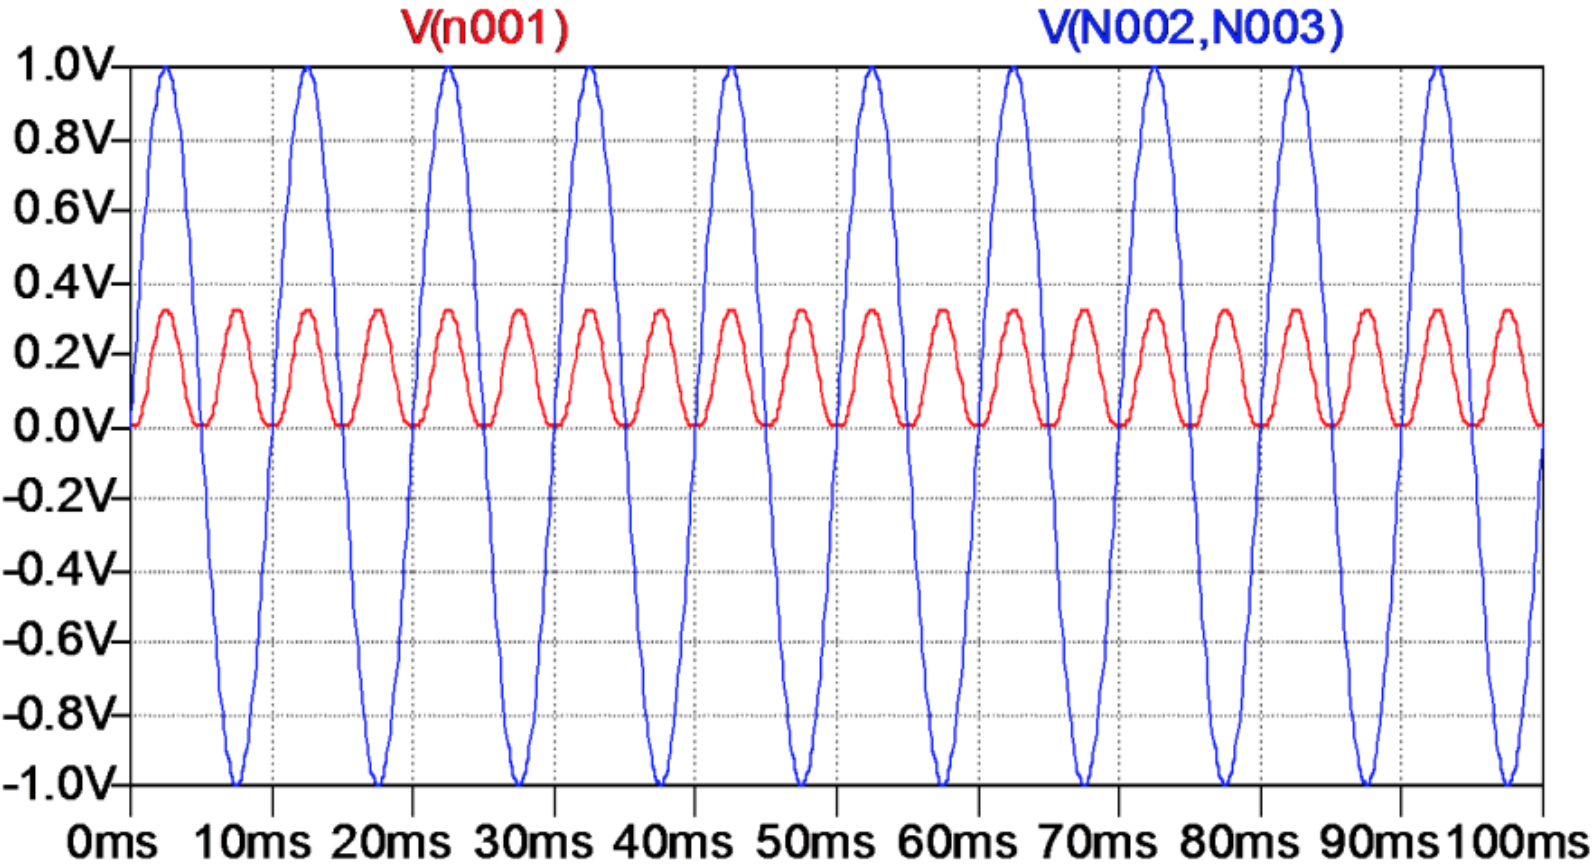
\includegraphics[width=.8\linewidth]{Figures/onda_silicon_rectifier}  
		\caption{Caída de tensión generada por el rectificador de la figura \ref{fig:rect_diodos}}
		\label{fig:onda_rectificador_diodos}
	\end{subfigure}
	\newline
	\begin{subfigure}{.5\textwidth}
		\centering
		% include third image
		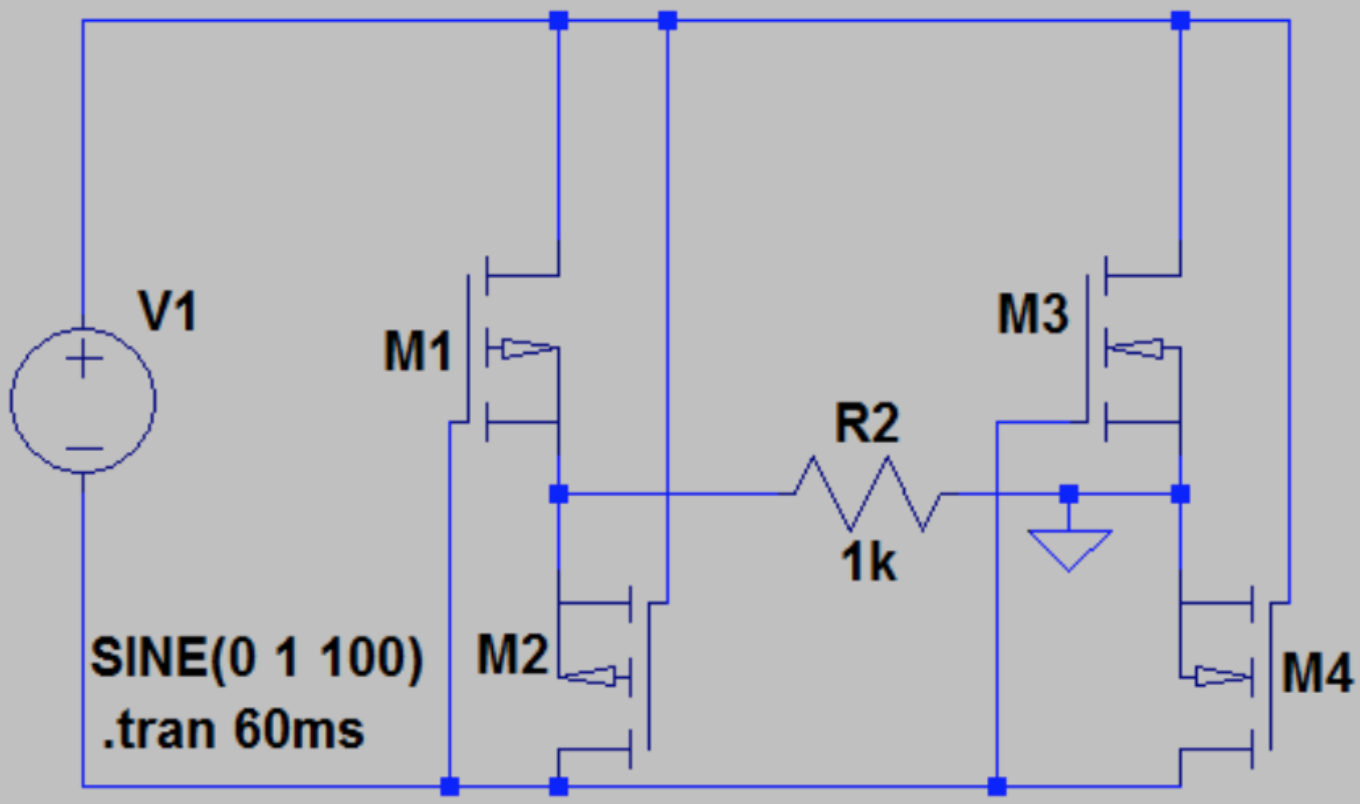
\includegraphics[width=.8\linewidth]{Figures/YILMAZ_passive_MOSFET_rectifier}  
		\caption{Rectificador basado en transistores MOSFET}
		\label{fig:rect_MOSFET}
	\end{subfigure}
	\begin{subfigure}{.5\textwidth}
		\centering
		% include fourth image
		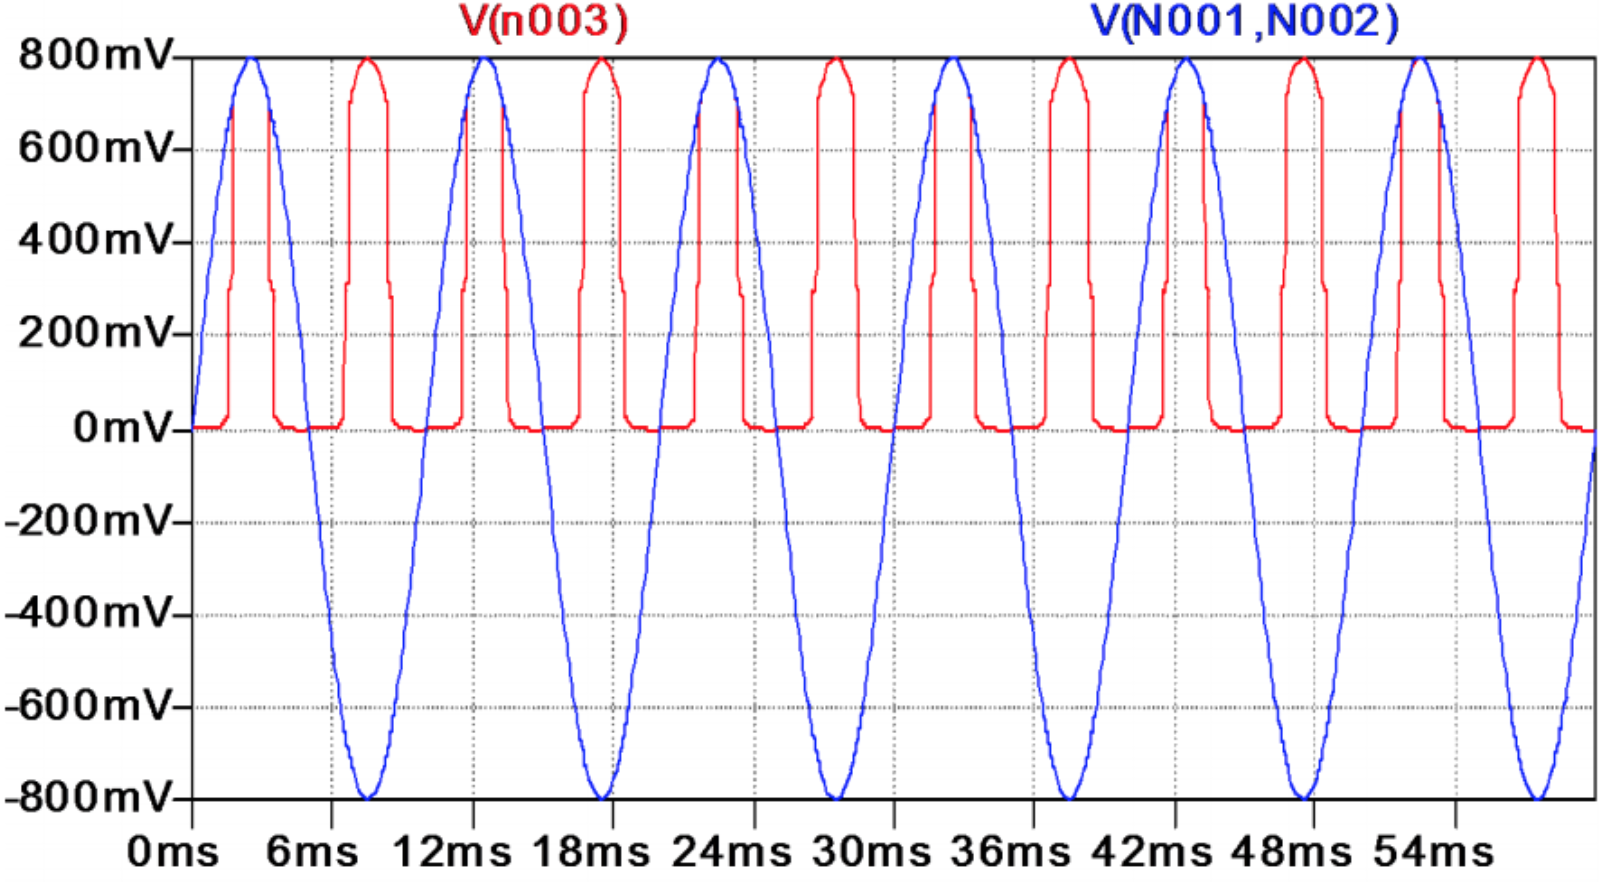
\includegraphics[width=.8\linewidth]{Figures/onda_passive_mosfet_rectifier}  
		\caption{Caída de tensión generada por el rectificador de la figura \ref{fig:rect_MOSFET}}
		\label{fig:onda_rectificador_MOSFET}
	\end{subfigure}
	\caption{Simulación de rectificadores basados en diodos y MOSFET. Imágenes tomadas de: \citep{Yilmaz}}
	\label{fig:comparacion_diodos_vs_MOSFET}
\end{figure}
Al comparar las simulaciones expuestas en las figuras \ref{fig:onda_rectificador_diodos} y \ref{fig:onda_rectificador_MOSFET} se aprecia que la caída de tensión generada por el rectificador basado en MOSFET al entrar en conducción es menor que uno hecho con diodos, por lo tanto también la potencia disipada en forma de calor.\\

\subsection{Supercapacitor como acumulador de energía}
La decisión de optar por un banco de supercapacitores (SC) como reemplazo total de una batería, se basa principalmente en el entorno donde operará el nodo HW. Diferencias entre una batería y un SC de interés para este proyecto, se plasman en la tabla \ref{tab:batteria_vs_supercap}.\\
Datos meteorológicos de la provincia de Misiones presentados en \citep{historico_temperaturas}, acusan temperaturas por encima de 30 C durante el periodo de septiembre a marzo. A diferencia de un SC que posee un rango de temperaturas de operación desde los -40 C hasta 70 C \citep{datasheet_supercap}, condiciones por encima de 35 grados son nocivas para una batería y generan el deterioro prematuro de sus componentes\citep{MA2018653}.\\
%\begin{verbatim}
\begin{table}[h]
	\centering
	\caption{Comparativa entre una batería y un supercapacitor para este proyecto}
	\begin{tabular}{lcc} 
		\hline
		\multicolumn{1}{c}{}                                                  & Batería         & Supercapacitor                                                                         \\ 
		\hline
		\begin{tabular}[c]{@{}l@{}}Densidad de \\energía (Wh/Kg)\end{tabular} & 265             & 3,9                                                                                    \\
		\begin{tabular}[c]{@{}l@{}}Rango de \\temperatura (C)\end{tabular}    & 15 a 35         & -40 a 70                                                                               \\
		Gestión de carga                                                      & V o I constante & \begin{tabular}[c]{@{}c@{}}Determinado por un\\circuito RC serie \citep{ceraolo2014fundamentals}\end{tabular}  \\
		\hline
	\end{tabular}
	\label{tab:batteria_vs_supercap}
\end{table}\\
%\end{verbatim}
Es importante remarcar que la densidad de energía que pueden almacenar también es diferente, una batería tiene una densidad de energía 60 veces mayor que un SC. Sin embargo, para esta aplicación puntual no representó un factor importante a la hora de elegir el acumulador.\\
Por último, el ciclo de carga es más complejo en el caso de una batería. Las etapas de su curva de carga deben ser respetados según sean a corriente o tensión constante. Esto trae acarreado implementar una electrónica adicional encargada de gestionar estos 2 parámetros. En un capacitor, la curva de carga está definida por un circuito RC serie \citep{ceraolo2014fundamentals}.\\ 

\subsection{Elevación de tensión mediante un conversor DC/DC }
Para proveer al MC, y el resto de la electrónica asociada de una tensión DC fija y constante, se ha optado por emplear un módulo comercial DC/DC ya existente en el mercado y es presentado en la figura \ref{fig:dcdcboost}.\\
% TODO: \usepackage{graphicx} required
\begin{figure}[h!]
	\centering
	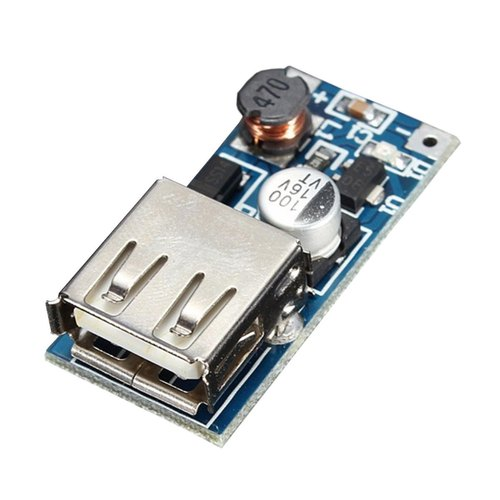
\includegraphics[width=0.4\linewidth]{Figures/dcdc_boost}
	\caption{Módulo comercial DC/DC en topología boost utilizado para alimentar la electrónica}
	\label{fig:dcdcboost}
\end{figure}\\
Su topología interna es \textit{boost} o elevador de tensión. En el HW del sistema, cumple la función de llevar la tensión variable del SC conectado a su entrada a una fija de 5 V. 
A su entrada admite tensiones variables desde 0,9 V hasta 5 V y puede otorgar hasta 500 miliamperes de corriente a la salida.

\subsection{Microcontrolador y firmware}
El MC es el ente encargado de ejecutar la lógica de negocios acorde a la tarea que debe cumplir el HW. En el mercado existe una amplia gama de fabricantes de placas de desarrollo que permiten acelerar la etapa de prototipado y validación de diseño.\\
La placa de desarrollo elegida para el prototipo fue la LoPy 4 producida por la firma Pycom y se presenta en la figura \ref{fig:lopy4} . En su interior alberga un ESP32, 8 Megabytes de memoria flash, transceptores de radio LoRa y 802.11 y un regulador de tensión.\\
\begin{figure}[h]
	\centering
	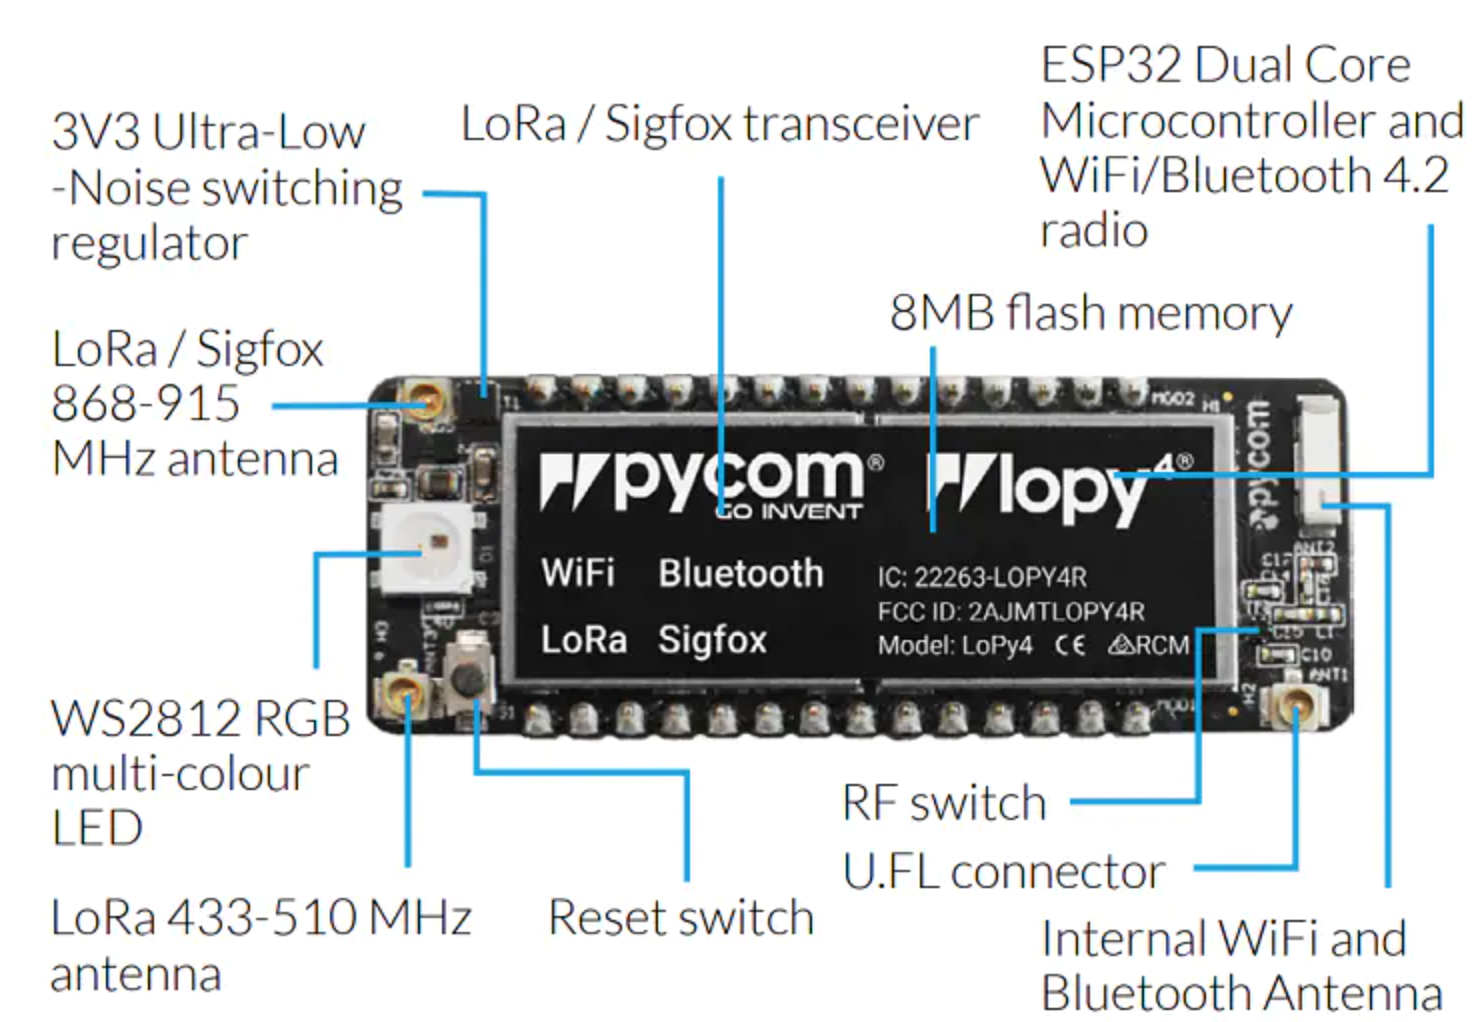
\includegraphics[width=0.7\linewidth]{Figures/lopy4}
	\caption{Placa de desarrollo LoPy 4 \citep{lopy4}}
	\label{fig:lopy4}
\end{figure}\\
El lenguaje de programación del LoPy4 es Micropython \citep{micropy}, un lenguaje de alto nivel lanzado por primera vez en el año 2014. Desde su lanzamiento y hasta la fecha de desarrollo de este trabajo, se presenta como una variante de Python atractiva para prototipar FW sobre microcontroladores utilizando el paradigma de programación orientada a objetos.\\


\section{Detalle del software}
\subsection{Red LoRaWAN}
LoRaWAN (Long Range Wide Area Network) es un protocolo de control de acceso al medio (MAC - \textit{Medium Acces Control}) definido por \textit{LoRa Aliance} \citep{lora_alliance}. Tiene por objeto permitir la conexión de nodos de baja potencia (generalmente alimentados a batería y sin capacidad de manejo de protocolos de enrutamiento por ejemplo TCP/IP) con aplicaciones finales conectadas a Internet mediante una conexión inalámbrica de largo alcance utilizando modulación LoRa.\\
Las puertas de enlace (GW - \textit{gateways}), están conectados al servidor central mediante conexiones IP (Internet Protocol) estándar cumpliendo la función de puente, es decir, convierte los paquetes de radiofrecuencia (RF) en paquetes IP y viceversa \ref{fig:arqlorawan}.\\
% TODO: \usepackage{graphicx} required
\begin{figure}[h]
	\centering
	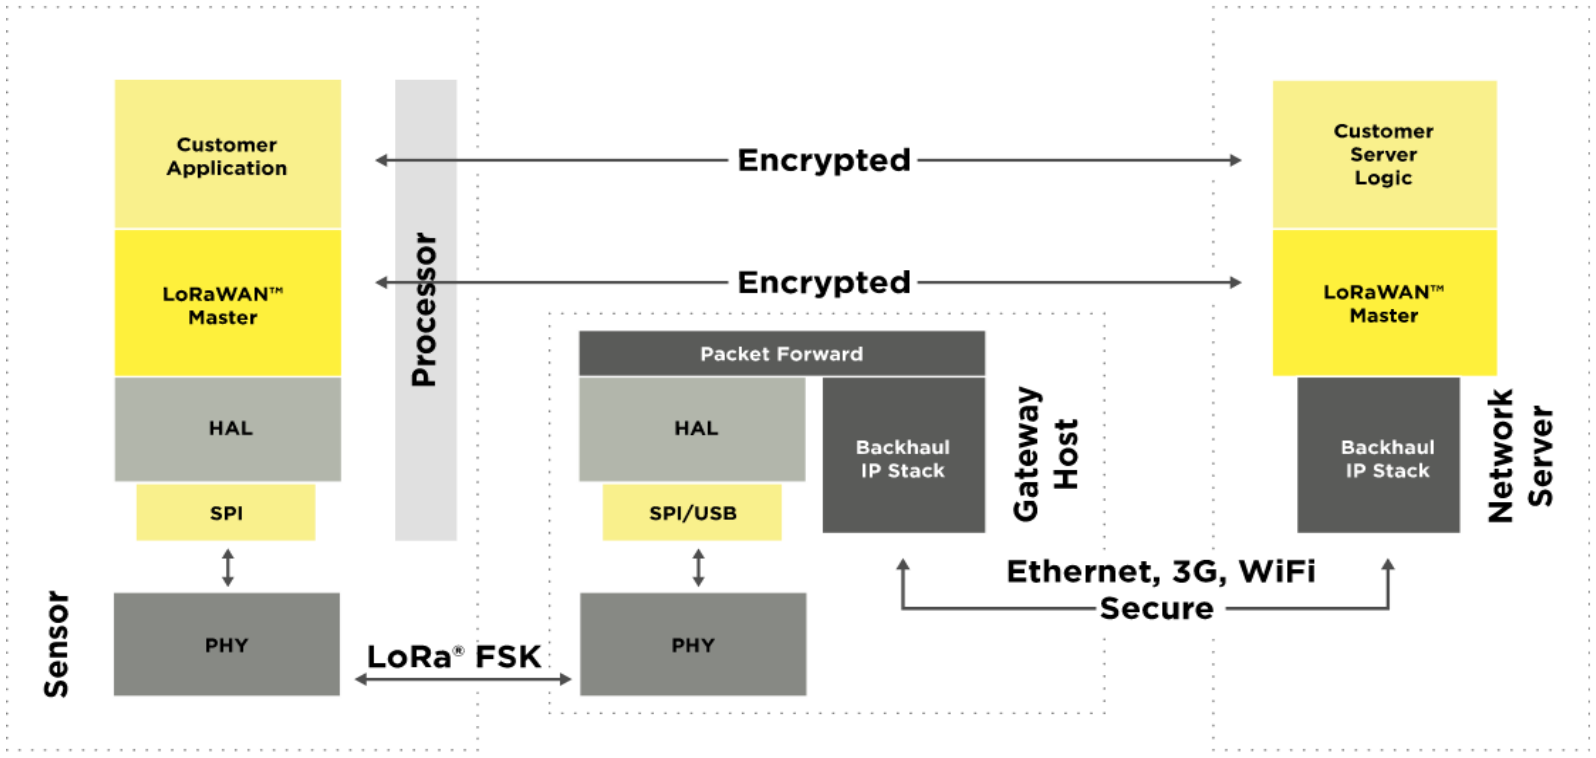
\includegraphics[width=0.9\linewidth]{Figures/arq_lorawan_2}
	\caption{Arquitectura de una red LoRaWAN y sus posibles integraciones con terceras partes \citep{lora_alliance}.}
	\label{fig:arqlorawan}
\end{figure}\\
El protocolo LoRaWAN no es un protocolo IP, por lo tanto, los paquetes del mismo necesitan de un enrutamiento y procesamiento correspondiente antes de ser entregados a la aplicación final.\\
La figura \ref{fig:sensor-gw-architecture-lora} presenta la topología tipo ``estrella de estrellas`` que adopta una red LoRaWAN. En ella los GW retransmiten los mensajes recibidos de los nodos finales hacia un servidor central. La comunicación inalámbrica entre nodos y GW aprovecha las características propias de la capa física, permitiendo así enlaces de un nodo hacia uno o más \textit{gateways}.\\
% TODO: \usepackage{graphicx} required
\begin{figure}[h]
	\centering
	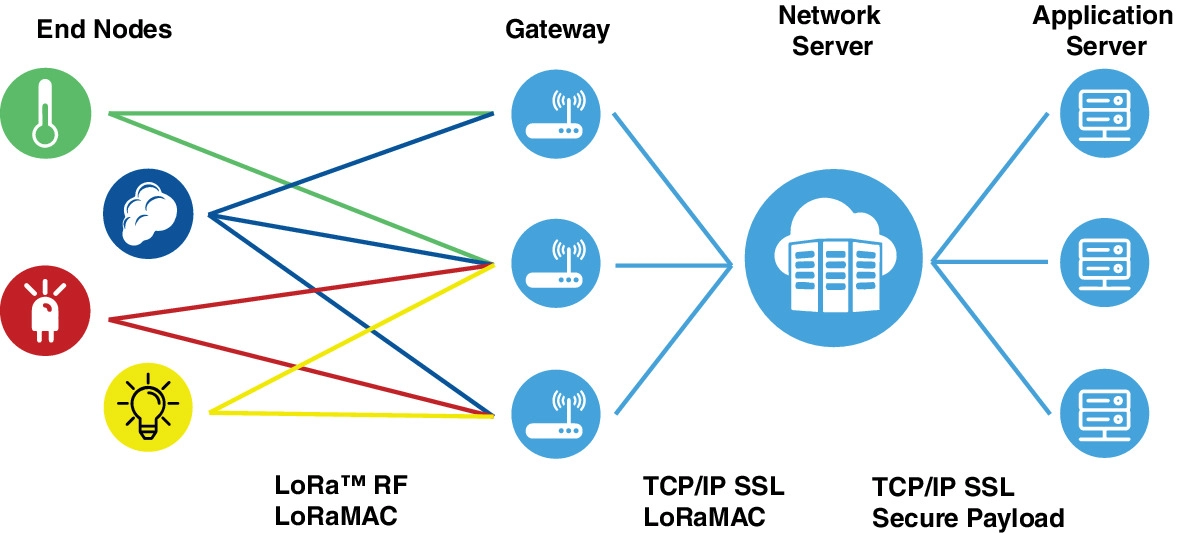
\includegraphics[width=0.9\linewidth]{Figures/sensor-gw-architecture-lora}
	\caption{Topología de una red LoRaWAN y la interacción entre los diferentes miembros \citep{lora_alliance}.}
	\label{fig:sensor-gw-architecture-lora}
\end{figure}

\subsection{Motor de base de datos}
Una base de datos (DB - \textit{Database}) almacena la información de manera ordenada en tablas o estructuras de datos. Las distintas aplicaciones pueden ejecutar consultas para solicitar la parte de esos datos que necesiten en ese momento.\\
Las bases de datos más utilizadas para aplicaciones web son las basadas en un modelo relacional, también conocidas como bases de datos SQL (Structured Query Language). Sin embargo, en años recientes se han popularizado las llamadas bases de datos NoSQL. Estas últimas están orientadas a documentos y almacena información de un mismo tipo en la forma de clave-valor.\\
Por su naturaleza, este proyecto parece indicado para utilizar NoSQL, ya que solo almacena registros de un tipo y no necesita crear relaciones complicadas entre distintas tablas de datos.\\
En principio se pensó en utilizar \textit{Elasticsearch} \citep{elasticsearch}, un servidor de búsqueda de texto basado en documentos JSON. Parecía el candidato ideal, ya que además de ser libre, se integraba perfectamente con Grafana, la herramienta para el desarrollo de la interfaz gráfica elegida \citep{grafana}.\\
Sin embargo, en las primeras pruebas llevadas a cabo se pudo apreciar que el consumo de memoria y procesamiento eran muy elevadas si se lo implementaba en un hardware modesto como las \textit{Raspberry Pi} \citep{raspi}. Finalmente se optó por utilizar MariaDB \citep{mariadb}, una base de datos del tipo SQL, también libre, con menos demanda de recursos y muy popular en aplicaciones web.\\

\subsection{Interfaz gráfica de usuario}
Una vez recuperados los datos de la red LoRaWAN y almacenados en la DB, una GUI presenta al usuario final del centro de operaciones los datos recolectados por cada nodo.\\
Una interfaz gráfica como la presentada en la figura \ref{fig:guirequeridaporelcliente}, se encarga de presentar al usuario final los últimos datos adquiridos por cada nodo. De esta manera, se puede identificar de manera simple mediante un punto verde o rojo sobre el mapa si la línea monitoreada presenta un problema.
% TODO: \usepackage{graphicx} required
\begin{figure}[h!]
	\centering
	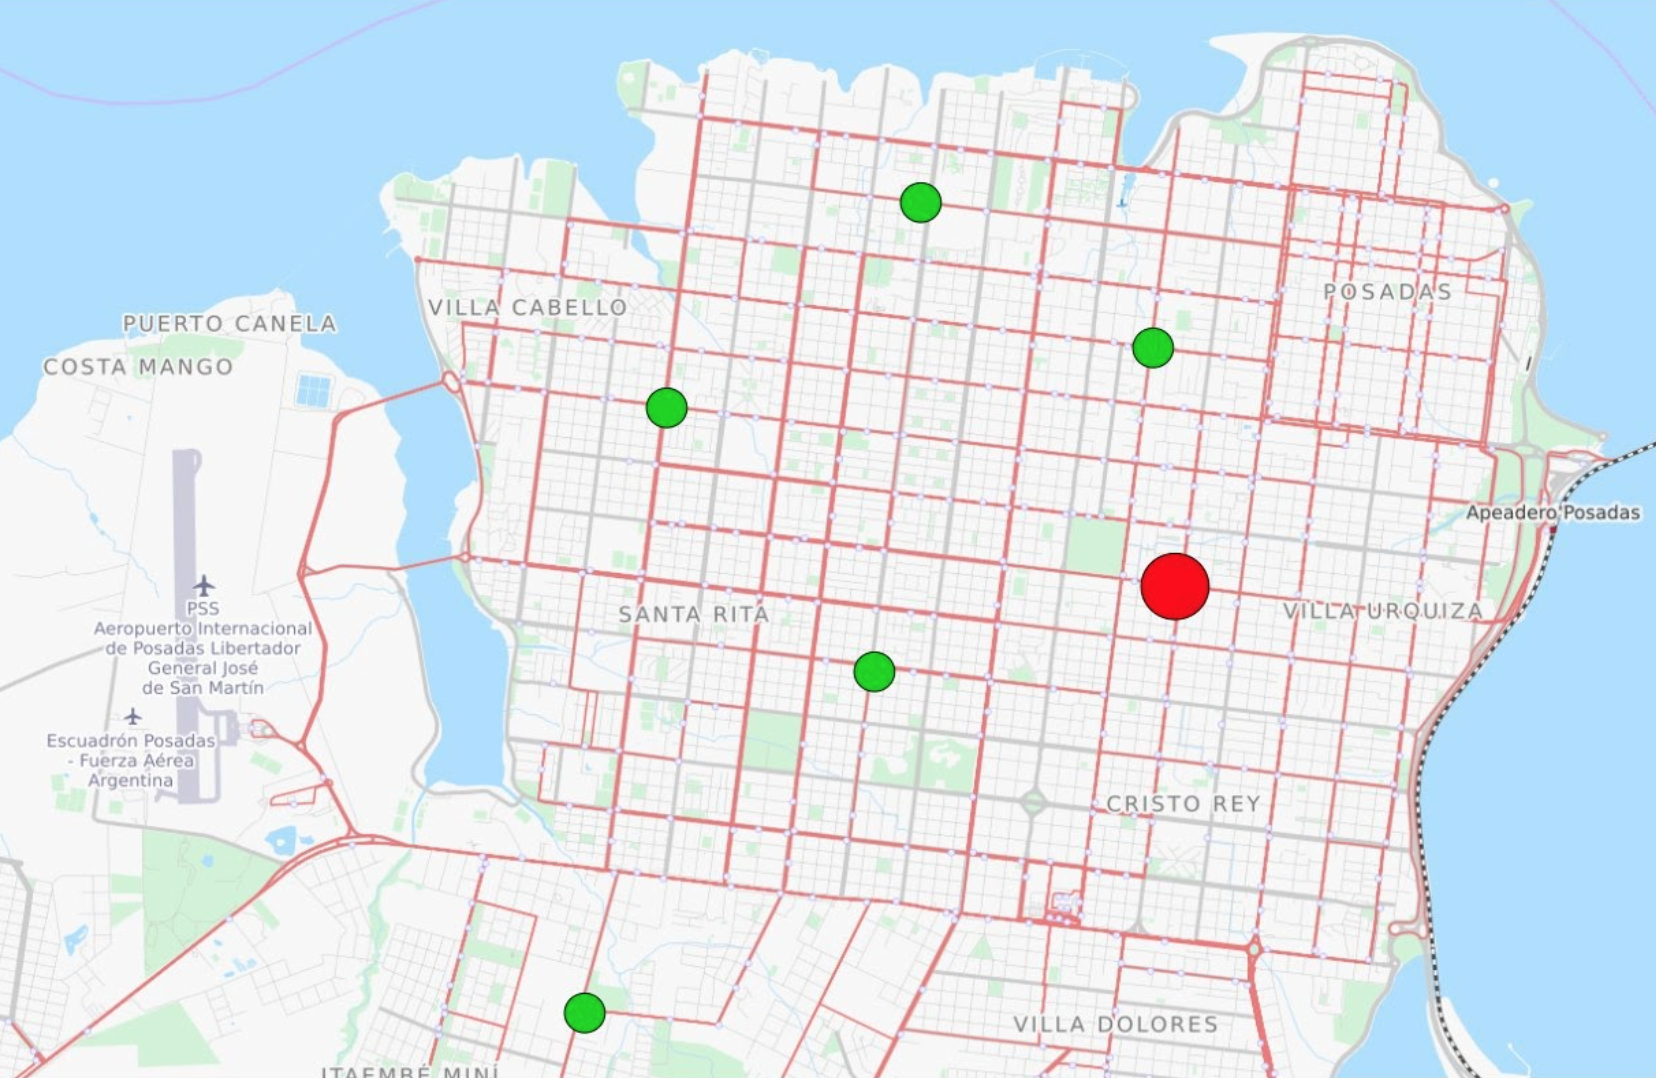
\includegraphics[width=0.7\linewidth]{Figures/GUI_requerida_por_el_cliente}
	\caption{Ejemplo de interfaz gráfica de usuario requerida por el cliente para presentar los últimos datos recuperados por cada nodo en la ciudad de Posadas, Misiones.}
	\label{fig:guirequeridaporelcliente}
\end{figure}\\
Para la presentación de la información se optó por Grafana, una aplicación web de código abierto para el análisis y visualización de datos, en especial datos temporales \citep{grafana}.\\
Grafana se adaptó muy bien a las necesidades del proyecto. Para mejorar aun más la experiencia del usuario se complementa con \textit{Worldmap Panel}, un \textit{plug in} que permite mostrar información temporal sobre un mapa. Esta información se presenta como círculos en las coordenadas donde se encuentra ubicado el nodo que genera la información.\\
 
	\chapter{Diseño e implementación} % Main chapter title

\label{Chapter3} % Change X to a consecutive number; for referencing this chapter elsewhere, use \ref{ChapterX}

\definecolor{mygreen}{rgb}{0,0.6,0}
\definecolor{mygray}{rgb}{0.5,0.5,0.5}
\definecolor{mymauve}{rgb}{0.58,0,0.82}

%%%%%%%%%%%%%%%%%%%%%%%%%%%%%%%%%%%%%%%%%%%%%%%%%%%%%%%%%%%%%%%%%%%%%%%%%%%%%
% parámetros para configurar el formato del código en los entornos lstlisting
%%%%%%%%%%%%%%%%%%%%%%%%%%%%%%%%%%%%%%%%%%%%%%%%%%%%%%%%%%%%%%%%%%%%%%%%%%%%%
\lstset{ %
  backgroundcolor=\color{white},   % choose the background color; you must add \usepackage{color} or \usepackage{xcolor}
  basicstyle=\footnotesize,        % the size of the fonts that are used for the code
  breakatwhitespace=false,         % sets if automatic breaks should only happen at whitespace
  breaklines=true,                 % sets automatic line breaking
  captionpos=b,                    % sets the caption-position to bottom
  commentstyle=\color{mygreen},    % comment style
  deletekeywords={...},            % if you want to delete keywords from the given language
  %escapeinside={\%*}{*)},          % if you want to add LaTeX within your code
  %extendedchars=true,              % lets you use non-ASCII characters; for 8-bits encodings only, does not work with UTF-8
  %frame=single,	                % adds a frame around the code
  keepspaces=true,                 % keeps spaces in text, useful for keeping indentation of code (possibly needs columns=flexible)
  keywordstyle=\color{blue},       % keyword style
  language=[ANSI]C,                % the language of the code
  %otherkeywords={*,...},           % if you want to add more keywords to the set
  numbers=left,                    % where to put the line-numbers; possible values are (none, left, right)
  numbersep=5pt,                   % how far the line-numbers are from the code
  numberstyle=\tiny\color{mygray}, % the style that is used for the line-numbers
  rulecolor=\color{black},         % if not set, the frame-color may be changed on line-breaks within not-black text (e.g. comments (green here))
  showspaces=false,                % show spaces everywhere adding particular underscores; it overrides 'showstringspaces'
  showstringspaces=false,          % underline spaces within strings only
  showtabs=false,                  % show tabs within strings adding particular underscores
  stepnumber=1,                    % the step between two line-numbers. If it's 1, each line will be numbered
  stringstyle=\color{mymauve},     % string literal style
  tabsize=2,	                   % sets default tabsize to 2 spaces
  title=\lstname,                  % show the filename of files included with \lstinputlisting; also try caption instead of title
  morecomment=[s]{/*}{*/}
}


%----------------------------------------------------------------------------------------
%	SECTION 1
%----------------------------------------------------------------------------------------
\section{Análisis del software}
 
La idea de esta sección es resaltar los problemas encontrados, los criterios utilizados y la justificación de las decisiones que se hayan tomado.

Se puede agregar código o pseudocódigo dentro de un entorno lstlisting con el siguiente código:

\begin{verbatim}
\begin{lstlisting}[caption= "un epígrafe descriptivo"]
	las líneas de código irían aquí...
\end{lstlisting}
\end{verbatim}

A modo de ejemplo:

\begin{lstlisting}[label=cod:vControl,caption=Pseudocódigo del lazo principal de control.]  % Start your code-block

#define MAX_SENSOR_NUMBER 3
#define MAX_ALARM_NUMBER  6
#define MAX_ACTUATOR_NUMBER 6

uint32_t sensorValue[MAX_SENSOR_NUMBER];		
FunctionalState alarmControl[MAX_ALARM_NUMBER];	//ENABLE or DISABLE
state_t alarmState[MAX_ALARM_NUMBER];						//ON or OFF
state_t actuatorState[MAX_ACTUATOR_NUMBER];			//ON or OFF

void vControl() {

	initGlobalVariables();
	
	period = 500 ms;
		
	while(1) {

		ticks = xTaskGetTickCount();
		
		updateSensors();
		
		updateAlarms();
		
		controlActuators();
		
		vTaskDelayUntil(&ticks, period);
	}
}
\end{lstlisting}




	% Chapter Template

\chapter{Ensayos y resultados} % Main chapter title

\label{Chapter4} % Change X to a consecutive number; for referencing this chapter elsewhere, use \ref{ChapterX}

%----------------------------------------------------------------------------------------
%	SECTION 1
%----------------------------------------------------------------------------------------

\section{PCB desarrollado}
\label{sec:pruebasHW}

\section{Medidor de valor RMS}\label{ensayo_medidor_rms}

\section{Circuito detector de cortes}

\section{Consumo en deep sleep}

\section{Autonom\'{i}a del supercapacitor}

\section{Ensayo end-to-end} 
	% Chapter Template

\chapter{Conclusiones} % Main chapter title

\label{Chapter5} % Change X to a consecutive number; for referencing this chapter elsewhere, use \ref{ChapterX}


%----------------------------------------------------------------------------------------

%----------------------------------------------------------------------------------------
%	SECTION 1
%----------------------------------------------------------------------------------------

\section{Conclusiones generales }
El sistema desarrollado, en concordancia con el objetivo general, conforma una herramienta económica para la prestadora del servicio de energía. Esta herramienta está diseñada para otorgar mayor granularidad de información sobre el estado de operación de las redes de distribución, sin implicar cambios significativos de infraestructura. Por otra parte, el análisis de la información suministrada permite identificar eventos recurrentes y evaluar sus posibles causas para poder delinear acciones correctivas y/o preventivas para mejorar la calidad de servicio.\\
Cumplimentando todos los requerimientos planteados por el cliente, y el tiempo planteado en la planificación, se ha logrado el desarrollo exitoso del sistema en todas sus partes: \textit{hardware}, \textit{firmware}, servicios de \textit{backend}; como así también su integración con la red LoRaWAN.\\
El uso de la red LPWAN de acceso público \textit{The Things Network} seleccionada para el trabajo, ha prestado servicios durante todo el desarrollo del proyecto sin solución de continuidad, demostrando así su buena cobertura y calidad de servicio a nivel global. A\'{u}n habiendo cambiado la localización geográfica de Europa a Sudamérica para realizar pruebas de laboratorio, la operación del sistema no se ha visto afectada en ningún aspecto.\\
El \textit{hardware} es capaz de convertir energía de corriente alterna proveniente del transformador de intensidad en otra de corriente continua y almacenarla. Los resultados del Capítulo 4, demuestran que el uso de circuitos de \textit{energy harvesting} en conjunto con tecnologías alternativas de acumulación en constante evolución como los supercapacitores, podrían ser sustitutos factibles de las baterías litio en aplicaciones autónomas que operen en régimen 24/7 y donde el rango de temperatura de operación necesaria sea mayor.\\
Las mediciones de valor RMS de corriente realizadas en el laboratorio, simulando la señal del TI con un generador de ondas y usando una carga de prueba presentadas en \ref{ensayo_medidor_rms}, demostraron la linealidad del circuito de medición dentro del rango de medición adoptado.\\
A partir de los ensayos de consumo en modo \textit{deep sleep} y autonomía de operación presentados en el capítulo \ref{Chapter4}, queda demostrado que el patrón \textit{power save loop} ha tenido un impacto significativamente positivo en la gestión de energía del nodo.\\
El tiempo total de propagación de datos desde el nodo \textit{in situ} hacia la red LoRaWAN, recuperación por los servicios de \textit{backend} y presentación en la interfaz gr\'{a}fica de usuario, es menor a 5 segundos. Este tiempo de propagación para el reporte de un problema, es considerado excelente en contraste con la situación actual en la provincia de Misiones.\\
Un conjunto de \textit{software} con abundante documentación tal como lo es LAMPP, ha ayudado a reducir el tiempo requerido para la puesta en funcionamiento de los servicios de \textit{backend} propios del proyecto y la integración con la red LoRaWAN a través de su API REST.\\
Durante la etapa de integración entre LoRaWAN y los servicios de \textit{backend}, fue destacable la importancia de la unificación del lenguaje de programación a Python en \'{e}ste proyecto. Además de su uso para el desarrollo del \textit{firmware}, se lo utilizó para implementar mockups que emulen los datos generados por el \textit{hardware}. Mediante el uso de esta técnica se pudo garantizar un flujo de desarrollo totalmente desacoplado de la necesidad de involucrar el \textit{hardware}, pero sí con una interacción constante entre servicios \textit{web} públicos y privados.\\


%----------------------------------------------------------------------------------------
%	SECTION 2
%----------------------------------------------------------------------------------------
\section{Trabajo a futuro}

Cumplidos los requerimientos y finalizado el trabajo propuesto, se han identificado las siguientes áreas de mejoras a futuro tanto en HW como SW:

\begin{itemize}
	\item Actualizar de manera inalámbrica el \textit{firmware} (OTA - \textit{Over The Air}): nuevas versiones del \textit{firmware} del microcontrolador aportarán nuevas funcionalidades, correcciones o mejoras sobre las ya existentes en nodos desplegados. Sin embargo, desarrollar esta funcionalidad es de alta prioridad antes de que el sistema llegue a una etapa de lanzamiento de producto. De esta manera, se prescindirá de la necesidad de intervenir físicamente cada nodo para actualizarlo.\\
	\item Modularizar el PCB para realizar mediciones de 3 fases: dado que los sistemas de distribución son trifásicos, el HW deberá también permitir realizar mediciones de corrientes sobre las 3 fases del sistema. Para lograr esto se debería proponer una modularización de la etapa de medición de valor RMS de corriente.\\
	\item Integrar servicios de mensajería instantánea: si bien la GUI permite de manera rápida identificar sobre un mapa el punto geográfico donde la red presenta un problema o su estado actual de operación, contar con una aplicación similar para dispositivos móviles será de utilidad para el personal encargado de cumplir horarios de guardia.\\
	
\end{itemize}

 
\end{verbatim}

Los apéndices también deben escribirse en archivos .tex separados, que se deben ubicar dentro de la carpeta \emph{Appendices}. Los apéndices vienen comentados por defecto con el caracter \code{\%} y para incluirlos simplemente se debe eliminar dicho caracter.

Finalmente, se encuentra el código para incluir la bibliografía en el documento final.  Este código tampoco debe modificarse. La metodología para trabajar las referencias bibliográficas se desarrolla en la sección \ref{sec:biblio}.
%----------------------------------------------------------------------------------------

\section{Bibliografía}
\label{sec:biblio}

Las opciones de formato de la bibliografía se controlan a través del paquete de latex \option{biblatex} que se incluye en la memoria en el archivo memoria.tex.  Estas opciones determinan cómo se generan las citas bibliográficas en el cuerpo del documento y cómo se genera la bibliografía al final de la memoria.

En el preámbulo se puede encontrar el código que incluye el paquete biblatex, que no requiere ninguna modificación del usuario de la plantilla, y que contiene las siguientes opciones:

\begin{lstlisting}
\usepackage[backend=bibtex,
	natbib=true, 
	style=numeric, 
	sorting=none]
{biblatex}
\end{lstlisting}

En el archivo \file{reference.bib} se encuentran las referencias bibliográficas que se pueden citar en el documento.  Para incorporar una nueva cita al documento lo primero es agregarla en este archivo con todos los campos necesario.  Todas las entradas bibliográficas comienzan con $@$ y una palabra que define el formato de la entrada.  Para cada formato existen campos obligatorios que deben completarse. No importa el orden en que las entradas estén definidas en el archivo .bib.  Tampoco es importante el orden en que estén definidos los campos de una entrada bibliográfica. A continuación se muestran algunos ejemplos:

\begin{lstlisting}
@ARTICLE{ARTICLE:1,
    AUTHOR="John Doe",
    TITLE="Title",
    JOURNAL="Journal",
    YEAR="2017",
}
\end{lstlisting}


\begin{lstlisting}
@BOOK{BOOK:1,
    AUTHOR="John Doe",
    TITLE="The Book without Title",
    PUBLISHER="Dummy Publisher",
    YEAR="2100",
}
\end{lstlisting}


\begin{lstlisting}
@INBOOK{BOOK:2,
    AUTHOR="John Doe",
    TITLE="The Book without Title",
    PUBLISHER="Dummy Publisher",
    YEAR="2100",
    PAGES="100-200",
}
\end{lstlisting}


\begin{lstlisting}
@MISC{WEBSITE:1,
    HOWPUBLISHED = "\url{http://example.com}",
    AUTHOR = "Intel",
    TITLE = "Example Website",
    MONTH = "12",
    YEAR = "1988",
    URLDATE = {2012-11-26}
}
\end{lstlisting}

Se debe notar que los nombres \emph{ARTICLE:1}, \emph{BOOK:1}, \emph{BOOK:2} y \emph{WEBSITE:1} son nombres de fantasía que le sirve al autor del documento para identificar la entrada. En este sentido, se podrían reemplazar por cualquier otro nombre.  Tampoco es necesario poner : seguido de un número, en los ejemplos sólo se incluye como un posible estilo para identificar las entradas.

La entradas se citan en el documento con el comando: 

\begin{verbatim}
\citep{nombre_de_la_entrada}
\end{verbatim}

Y cuando se usan, se muestran así: \citep{ARTICLE:1}, \citep{BOOK:1}, \citep{BOOK:2}, \citep{WEBSITE:1}.  Notar cómo se conforma la sección Bibliografía al final del documento. 

	\chapter{Introducción específica} % Main chapter title
\label{Chapter2}
%----------------------------------------------------------------------------------------
%	SECTION 1
%----------------------------------------------------------------------------------------
En este capítulo se presentan los requerimientos acordados con el cliente y los recursos de \textit{hardware} (HW) y \textit{software} (SW) utilizados para el desarrollo del trabajo. Se describen en las partes implementadas del HW, los servicios integrados de \textit{backend} (BES) y solamente algunos aspectos relevantes del \textit{firmware} (FW) que interactúa con el HW. En el capítulo 3 se abarca la lógica de negocios implementada en el FW del microcontrolador.\\
\section{Requerimientos acordados con el cliente}
\label{sec:requerimientos}
\begin{enumerate}
	\item Grupo de requerimientos asociados con hardware
	\begin{enumerate}
		\item El dispositivo deberá ser de tipo \textit{plug and play}.
		\item El circuito impreso no deberá ocupar un volumen mayor a 10x10x5 cm.
		\item Basarse en un microcontrolador ESP32 y disponer de:
		\begin{enumerate}%[label*=\arabic*.]
			\item 4 entradas analógicas.
			\item 3 salidas digitales.
			\item Unidad UART.
			\item Integrar un módulo de comunicaciones LoRa.
		\end{enumerate}
		\item Deberá tener al menos 12 horas de autonomía de funcionamiento.
		\item Bajo consumo en modo ocioso: el consumo del hardware en total, no deberá superar los 5 mA cuando no está midiendo ni transmitiendo.
		\item El circuito elevador de tensión DC-DC deberá:
		\begin{enumerate}%[label*=\arabic*.]
			\item Funcionar con tensiones menores a 2V en la entrada.
			\item Otorgar 5 Volts a la salida.
			\item Ser capaz de otorgar 300 miliamperes a la salida.
		\end{enumerate}
		\item El transformador de corriente (TI) debe:
		\begin{enumerate}%[label*=\arabic*.]
			\item Ser de tipo núcleo partido.
			\item Admitir 100 Amperes de corriente en el circuito primario y un máximo 5 Amperes en el circuito secundario.
		\end{enumerate}
		\item \label{req_relay} El relay encargado de cambiar el modo de operación debe:
		\begin{enumerate}%[label*=\arabic*.]
			\item Ser de tipo doble inversor sin retención.
			\item Su bobina debe poder energizarse con 5V o menos.
			\item Soportar al menos 5 Amperes de corriente por los contactos.
		\end{enumerate} 
		\item Debe funcionar de manera independiente a la frecuencia de operación de la red 50/60 Hz.
		\item Debe funcionar de manera independiente a la tensión de fase del sistema de distribución 110/220 Voltios.
	\end{enumerate}
	\item Grupo de requerimientos asociados con el firmware
	\begin{enumerate}
		\item Debe manejar un módulo de comunicación LoRa y protocolo LoRaWAN.
		\item Deberá tener un porcentaje de cobertura de tests unitarios del 60\% como mínimo.
		\item Antes configurarse en modo ocioso, debe desenergizar la etapa de medición de corriente y el módulo de comunicaciones con el objeto de ahorrar energía.
	\end{enumerate}
	
	\item Grupo de requerimientos asociados con los servicios de backend (BES)
	\label{requerimientos_backend}
	\begin{enumerate}
		\item Todos los servicios deben poder correr en una Raspberry Pi 3.
		\item El \textit{software} de los BES se desarrollará en lenguaje Python.
		\item Recuperar los datos de la red LoRaWAN.\label{requerimiento_LORAWAN}
		\item Almacenar los datos en una tabla de MySQL.
		\item (GUI - \textit{Graphical User Interface}) basada en Grafana.
	\end{enumerate}
	
	\item Grupo de requerimientos asociados con ensayos de integración y \textit{end-to-end}
	\begin{enumerate}
		\item El banco de ensayos de \textit{hardware} debe contar con una carga fantasma de al menos 10 Amperes y permitir realizar interrupciones de corriente de manera programada mediante una computadora adicional tipo Raspberry Pi o de manera manual.
		\item Los BES deben estar operativos al momento de realizar los ensayos.
		\item Contar con un gateway de acceso a una red LoRaWAN como por ejemplo \textit{The Things Network}.
	\end{enumerate}
\end{enumerate}


\section{Diagrama de bloques general del sistema implementado}
El diagrama de bloques del HW a instalar \textit{in situ} es presentado en la figura \ref{fig:diagramadebloquesdelhw} y consta de cuatro bloques:
% TODO: \usepackage{graphicx} required
\begin{figure}[h!]
	\centering
	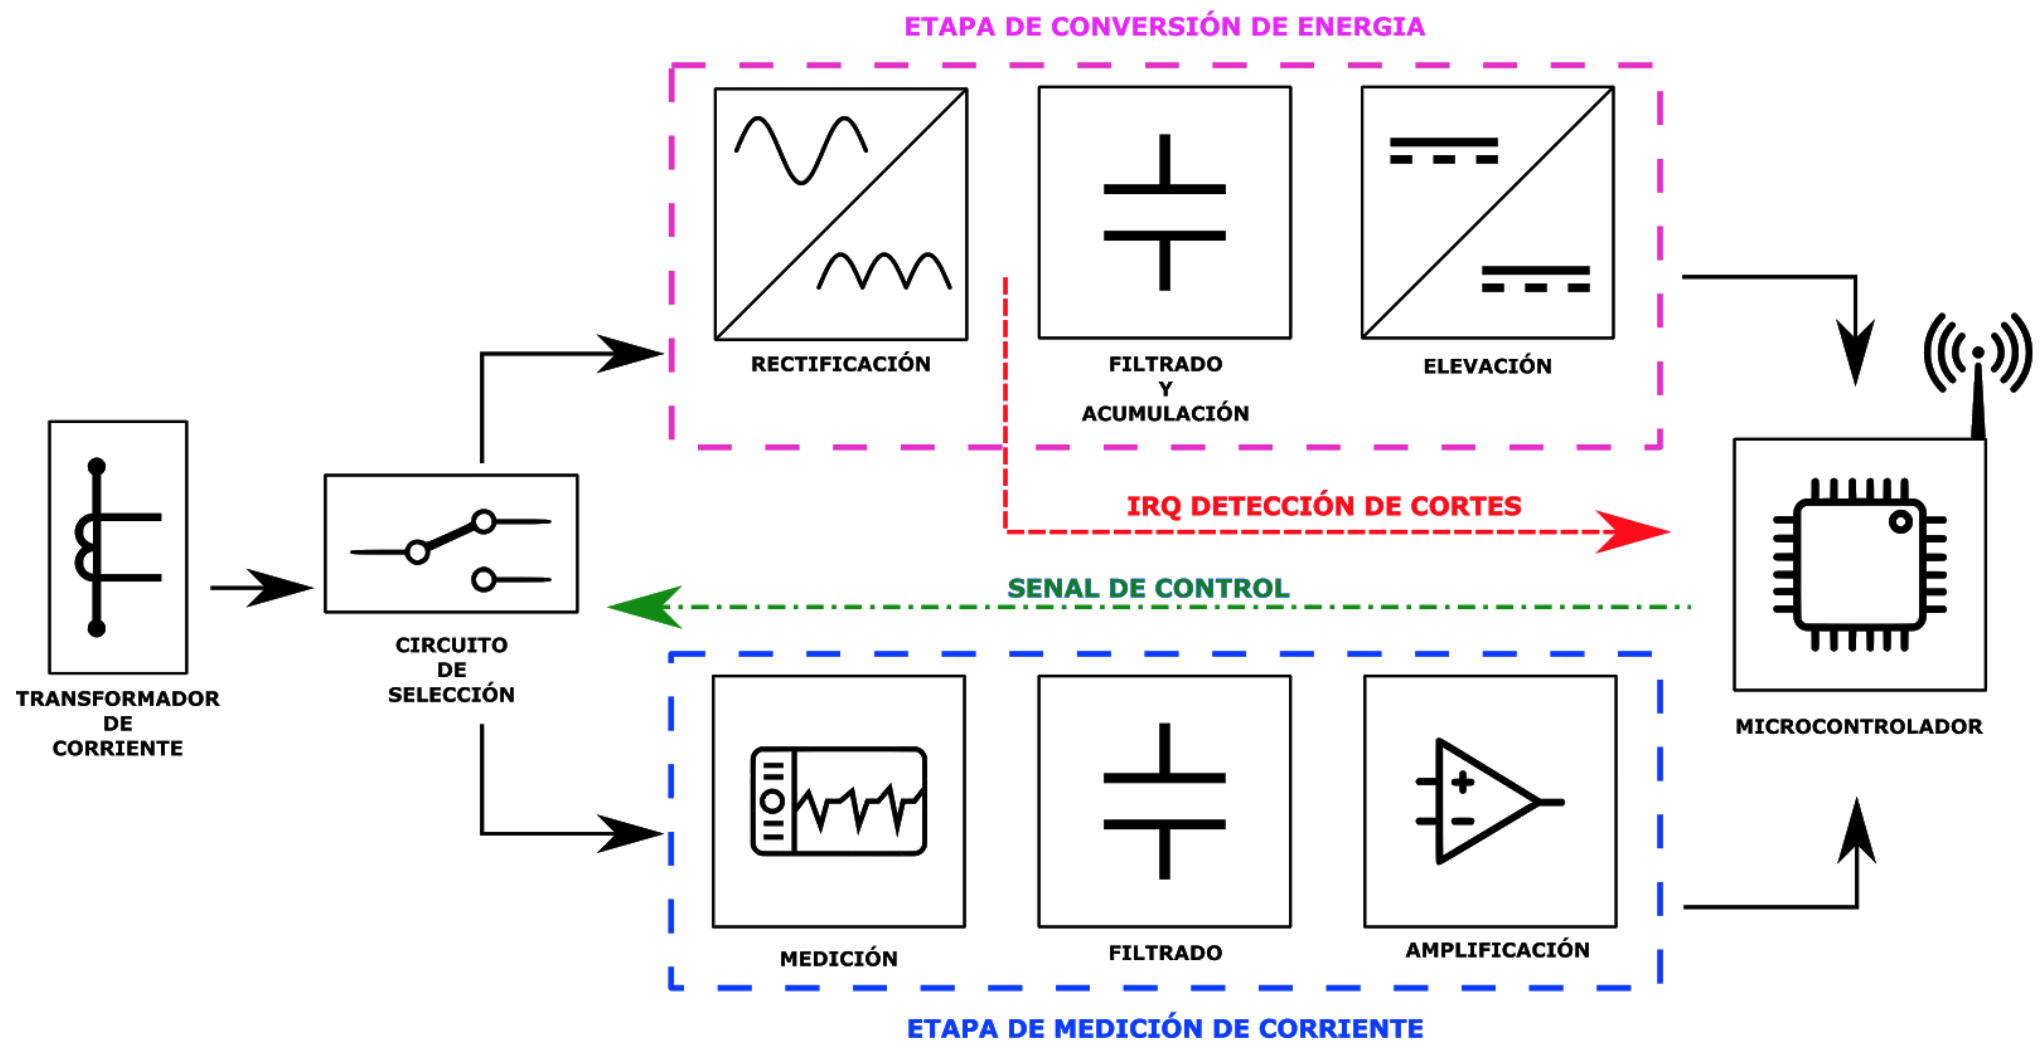
\includegraphics[width=0.7\linewidth]{Figures/diagrama_de_bloques_del_HW}
	\caption{Diagrama de bloques del HW para el nodo a instalar \textit{in situ}}
	\label{fig:diagramadebloquesdelhw}
\end{figure}
\begin{enumerate}
	\item Circuito de selección de modo: un relay (RL) y su circuito de mando controlarán a que etapa del nodo se conectarán los terminales del TI.
	\item Etapa de rectificación, acumulación de energía y elevación de tensión: compuesta por rectificador de onda completa, una etapa de filtrado y acumulación y un circuito elevador de tensión.
	\item Etapa de medición de valor RMS de corriente: un chip dedicado toma la señal de tensión generada en bornes del resistor shunt y calcula el valor RMS. A su salida entrega un valor proporcional de tensión DC.
	\item Microcontrolador (MC): ejecuta la lógica de negocios que rige el comportamiento del nodo, digitalizar mediciones y transmitir datos a la red LoRaWAN.
\end{enumerate}
Por otro lado, el sistema también implicó el desarrollo y puesta en funcionamiento de un conjunto de servicios de \textit{backend} (BES) propios del proyecto que cumplen las funciones de:
\begin{itemize}
	\item Recuperación de datos de la red LoRaWAN.
	\item Almacenamiento en una base de datos (DB).
	\item Presentación de los datos al usuario final mediante una interfaz gráfica de usuario (GUI).
\end{itemize}

El requisito \ref{requerimiento_LORAWAN} impuso el uso de una red LoRaWAN como columna vertebral para la transmisión de datos generados por los nodos. Para cumplirlo se adoptó la arquitectura presentada en la figura \ref{fig:diagramadebloquesdebes}.\\
% TODO: \usepackage{graphicx} required
\begin{figure}[h!]
	\centering
	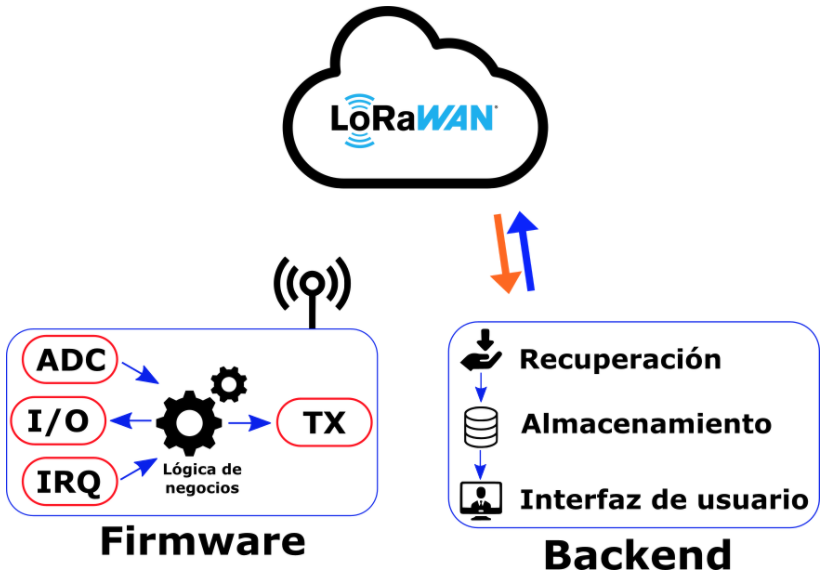
\includegraphics[width=0.6\linewidth]{Figures/diagrama_de_bloques_de_BES}
	\caption{Diagrama de bloques del FW implementado en el MC y su interacción con la red LoRaWAN y los BES privados del sistema.}
	\label{fig:diagramadebloquesdebes}
\end{figure}\\
Las mediciones son tomadas por el HW y transmitidas hacia la red LoRaWAN para luego interactuar con los BES privados que se encargan de recuperar, almacenar y presentar los datos al usuario final.\\


\section{Detalle del hardware}
\subsection{Transformador de corriente}
Un transformador de corriente o intensidad (TI) es un dispositivo de medición utilizado para producir en su devanado secundario una corriente diferente y proporcional a la que circula por su devanado primario.\\
El principio de operación de un TI no es diferente al de un transformador de potencia convencional. A diferencia de uno de potencia, el devanado primario puede ser de una sola vuelta sobre un núcleo ferromagnético como se ve en la figura \ref{fig:dibujomedicionti}. El devanado secundario suele tener un número mayor de vueltas alrededor del núcleo y depende de que tanto se debe reducir la corriente.\\
% TODO: \usepackage{graphicx} required
\begin{figure}[h!]
	\centering
	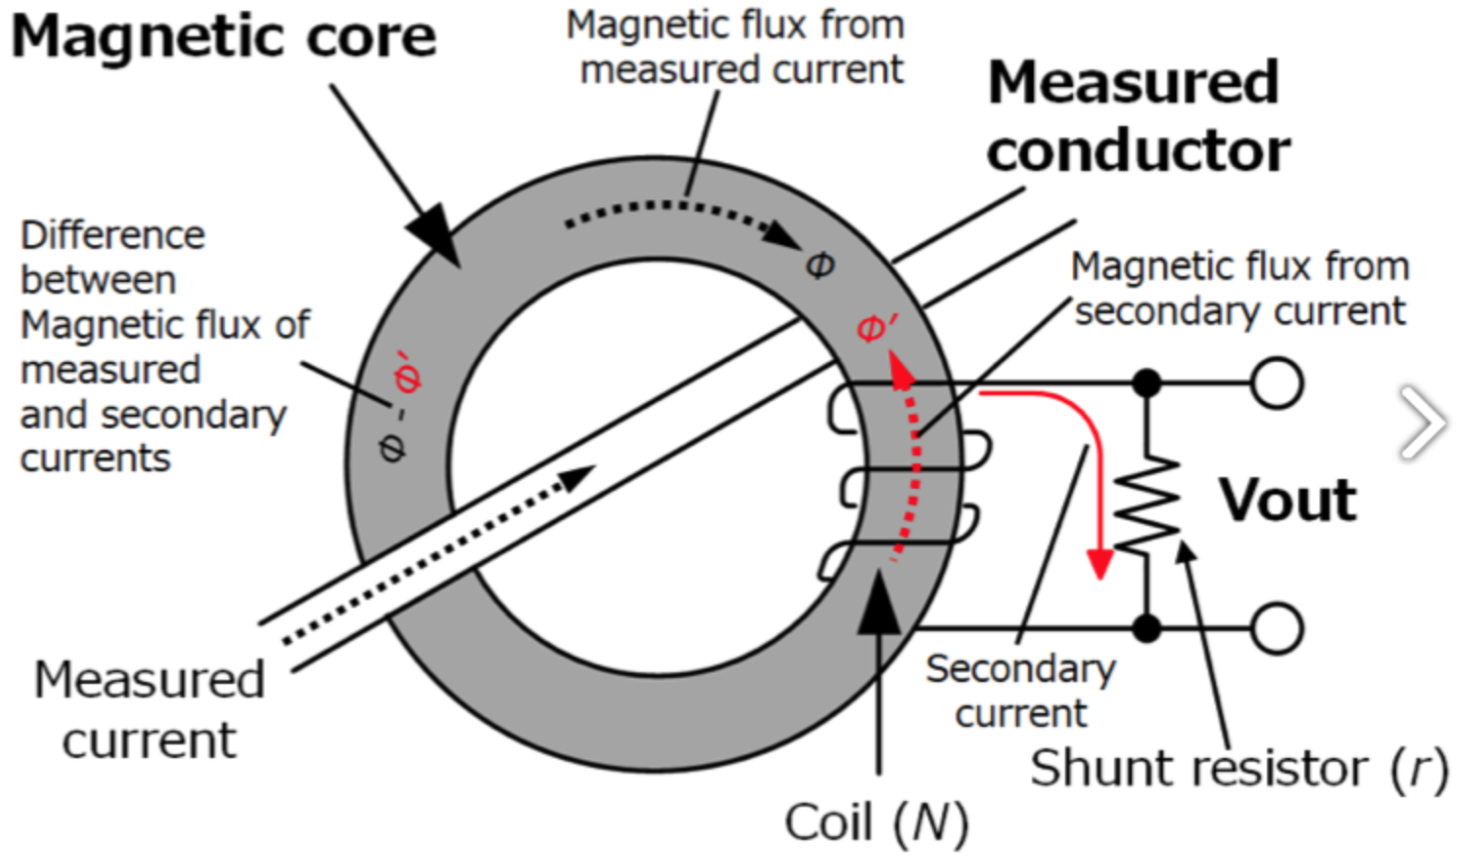
\includegraphics[width=0.5\linewidth]{Figures/dibujo_medicion_TI}
	\caption{Circuito de medición indirecta de corriente mediante un TI.\citep{hioki}}
	\label{fig:dibujomedicionti}
\end{figure}\\
Muchos TI tienen una relación estándar de 5 Amperes en el secundario, por ejemplo un TI 200/5 significa que cuando por el primario fluyen 200 amperes en el secundario solo fluyen 5. Es decir, el TI tiene una relación de transformación de corriente N de 40 veces.\\
Mediante esta técnica, pequeños instrumentos pueden monitorear grandes valores de corriente manteniendo una distancia segura de las líneas de alta tensión.


\subsection{Circuito de selección}
A partir del lineamiento de que el TI debe estar conectado por defecto a la entrada del rectificador y al resistor shunt al energizarse la bobina del RL, el número y la disposición de los contactos fue un factor relevante al momento de elegir la mejor opción. La variante comercial que cumplió con los requisitos \ref{req_relay} es la producida por la firma Hongfa modelo HF115F/005-2ZS4A presentada en la figura \ref{fig:relay}.
\begin{figure}[h!]
    \centering
	\begin{subfigure}[b]{0.3\textwidth}
		\centering
		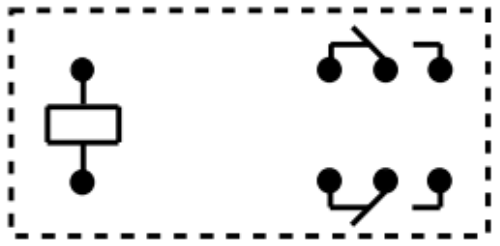
\includegraphics[width=.65\textwidth]{./Figures/relay_pinout}
		\caption{}
		\label{fig:relay_pinout}
	\end{subfigure}
    \centering
	\begin{subfigure}[b]{0.3\textwidth}
		\centering
		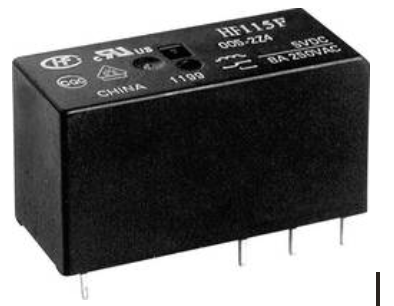
\includegraphics[width=.65\textwidth]{./Figures/relay_encapsulado}
		\caption{}
		\label{fig:relay_encapsulado}
	\end{subfigure}
	\caption{Pinout del relay HF115F/005-2ZS4A (izquireda) y su encapsulado (derecha). Imágenes tomadas de \citep{datasheet_relay}}
	\label{fig:relay}
\end{figure}

\subsection{Conversión de energía}
Para obtener una tensión continua a partir de una alterna generada por el TI, es necesario implementar un puente rectificador de onda completa.\\
En la actualidad la mayoría de los circuitos rectificadores de onda completa se basan en diodos de silicio de bajo costo. Sin embargo, un diodo de silicio posee una caída de tensión típica de 0,7 V. Esta caída de tensión se traduce en pérdidas por efecto Joule y es relevante en dispositivos donde la conversión, acumulación y gestión de energía es crítica. Por lo tanto, se desea maximizar la transferencia de tensión y potencia entre entrada y salida del puente rectificador.\\
Yilmaz \citep{Yilmaz} analiza técnicas de rectificación de onda completa con diferentes tipos de diodos, como así también un arreglo de transistores MOSFET pasivo y activo. Las caídas de tensión simuladas entre la entrada y salida entre un puente rectificador de diodos de silicio y uno pasivo basado en MOSFETs se comparan en la figura \ref{fig:comparacion_diodos_vs_MOSFET}.\\

\begin{figure}[h!]
	\begin{subfigure}{.5\textwidth}
		\centering
		% include first image
		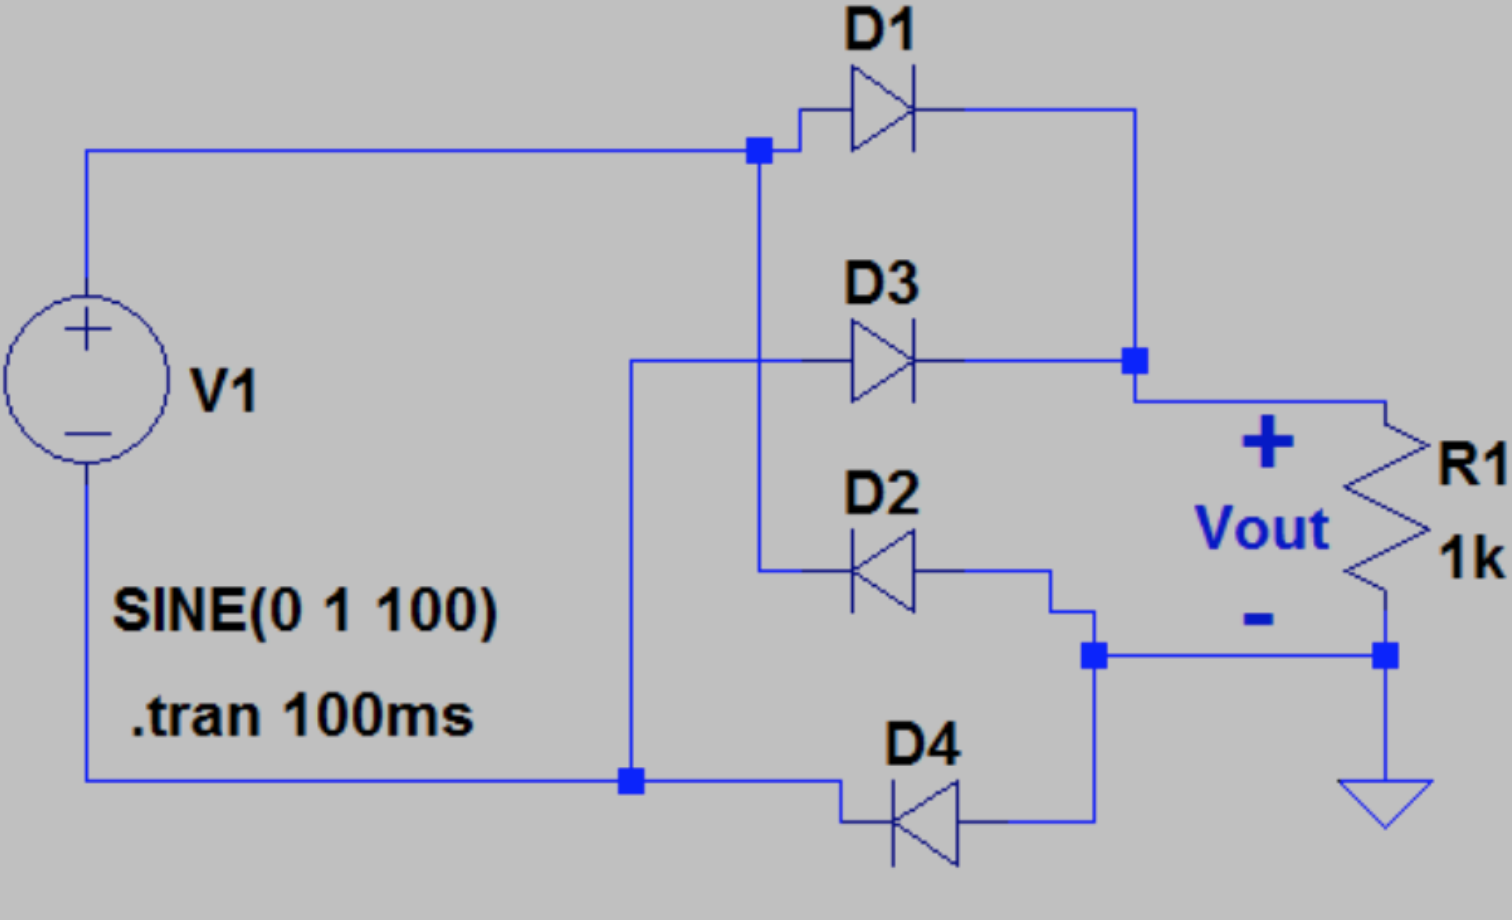
\includegraphics[width=.8\linewidth]{Figures/YILMAZ_silicon_diode_rectifier}  
		\caption{Rectificador basado en diodos de silicio}
		\label{fig:rect_diodos}
	\end{subfigure}
	\begin{subfigure}{.5\textwidth}
		\centering
		% include second image
		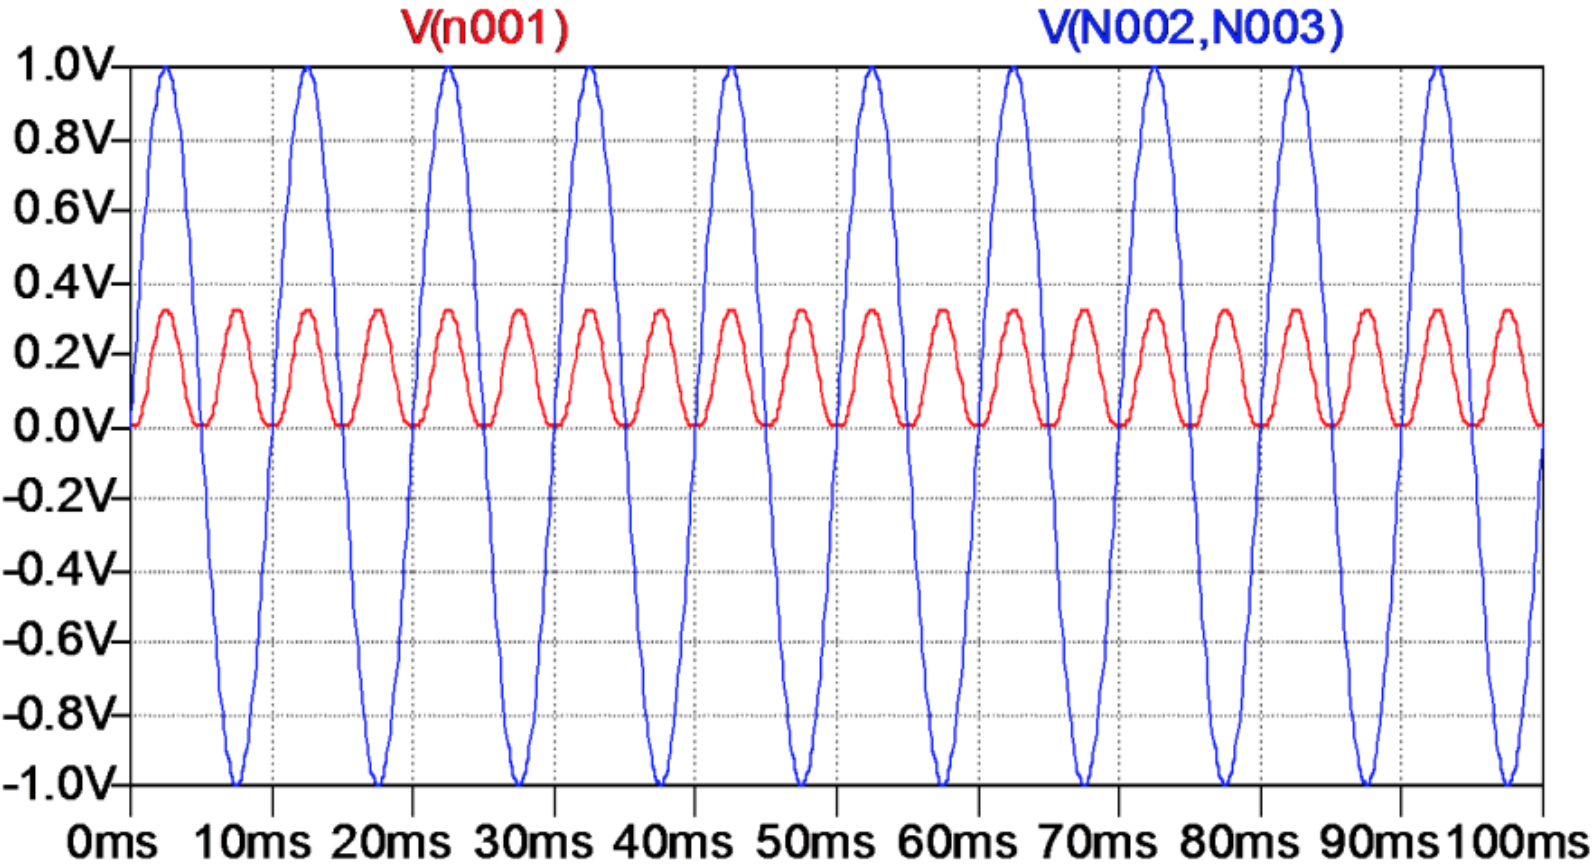
\includegraphics[width=.8\linewidth]{Figures/onda_silicon_rectifier}  
		\caption{Caída de tensión generada por el rectificador de la figura \ref{fig:rect_diodos}}
		\label{fig:onda_rectificador_diodos}
	\end{subfigure}
	\newline
	\begin{subfigure}{.5\textwidth}
		\centering
		% include third image
		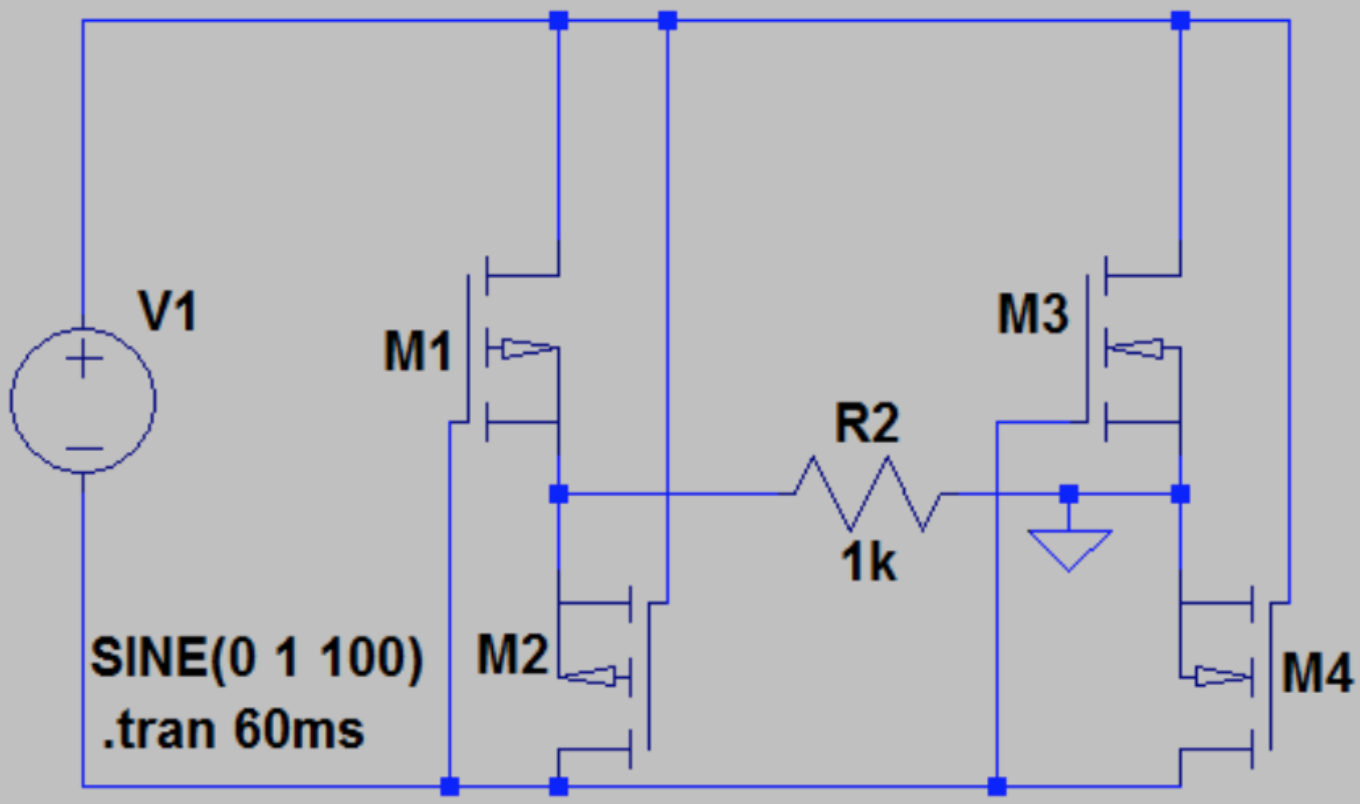
\includegraphics[width=.8\linewidth]{Figures/YILMAZ_passive_MOSFET_rectifier}  
		\caption{Rectificador basado en transistores MOSFET}
		\label{fig:rect_MOSFET}
	\end{subfigure}
	\begin{subfigure}{.5\textwidth}
		\centering
		% include fourth image
		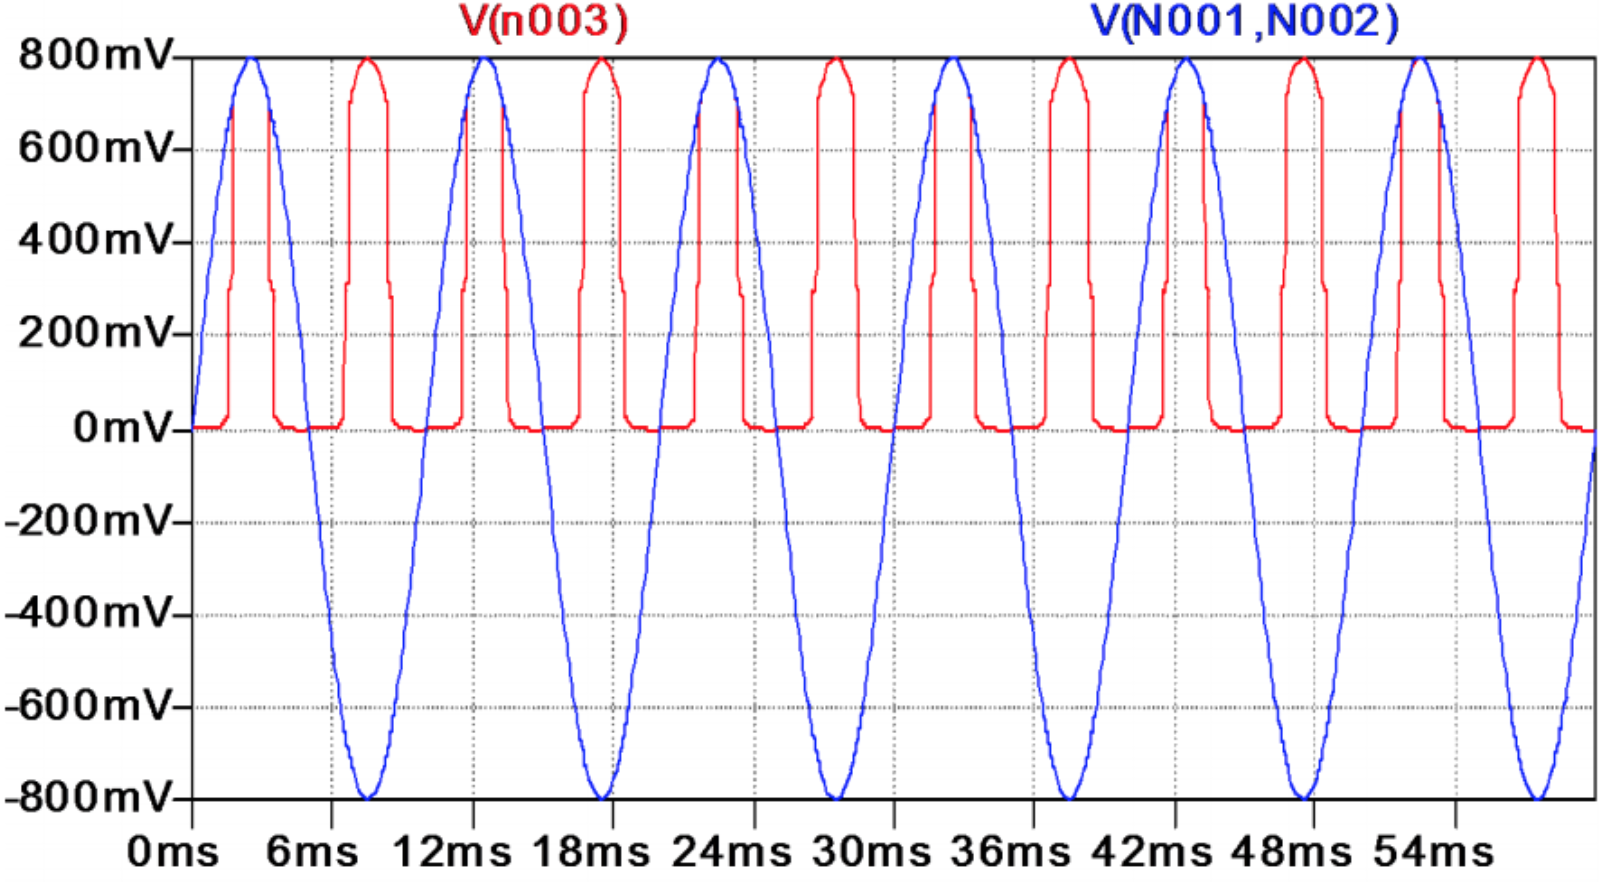
\includegraphics[width=.8\linewidth]{Figures/onda_passive_mosfet_rectifier}  
		\caption{Caída de tensión generada por el rectificador de la figura \ref{fig:rect_MOSFET}}
		\label{fig:onda_rectificador_MOSFET}
	\end{subfigure}
	\caption{Simulación de rectificadores basados en diodos y MOSFET. Imágenes tomadas de: \citep{Yilmaz}}
	\label{fig:comparacion_diodos_vs_MOSFET}
\end{figure}
Al comparar las simulaciones expuestas en las figuras \ref{fig:onda_rectificador_diodos} y \ref{fig:onda_rectificador_MOSFET} se aprecia que la caída de tensión generada por el rectificador basado en MOSFET al entrar en conducción es menor que uno hecho con diodos, por lo tanto también la potencia disipada en forma de calor.\\

\subsection{Supercapacitor como acumulador de energía}
La decisión de optar por un banco de supercapacitores (SC) como reemplazo total de una batería, se basa principalmente en el entorno donde operará el nodo HW. Diferencias entre una batería y un SC de interés para este proyecto, se plasman en la tabla \ref{tab:batteria_vs_supercap}.\\
Datos meteorológicos de la provincia de Misiones presentados en \citep{historico_temperaturas}, acusan temperaturas por encima de 30 C durante el periodo de septiembre a marzo. A diferencia de un SC que posee un rango de temperaturas de operación desde los -40 C hasta 70 C \citep{datasheet_supercap}, condiciones por encima de 35 grados son nocivas para una batería y generan el deterioro prematuro de sus componentes\citep{MA2018653}.\\
%\begin{verbatim}
\begin{table}[h]
	\centering
	\caption{Comparativa entre una batería y un supercapacitor para este proyecto}
	\begin{tabular}{lcc} 
		\hline
		\multicolumn{1}{c}{}                                                  & Batería         & Supercapacitor                                                                         \\ 
		\hline
		\begin{tabular}[c]{@{}l@{}}Densidad de \\energía (Wh/Kg)\end{tabular} & 265             & 3,9                                                                                    \\
		\begin{tabular}[c]{@{}l@{}}Rango de \\temperatura (C)\end{tabular}    & 15 a 35         & -40 a 70                                                                               \\
		Gestión de carga                                                      & V o I constante & \begin{tabular}[c]{@{}c@{}}Determinado por un\\circuito RC serie \citep{ceraolo2014fundamentals}\end{tabular}  \\
		\hline
	\end{tabular}
	\label{tab:batteria_vs_supercap}
\end{table}\\
%\end{verbatim}
Es importante remarcar que la densidad de energía que pueden almacenar también es diferente, una batería tiene una densidad de energía 60 veces mayor que un SC. Sin embargo, para esta aplicación puntual no representó un factor importante a la hora de elegir el acumulador.\\
Por último, el ciclo de carga es más complejo en el caso de una batería. Las etapas de su curva de carga deben ser respetados según sean a corriente o tensión constante. Esto trae acarreado implementar una electrónica adicional encargada de gestionar estos 2 parámetros. En un capacitor, la curva de carga está definida por un circuito RC serie \citep{ceraolo2014fundamentals}.\\ 

\subsection{Elevación de tensión mediante un conversor DC/DC }
Para proveer al MC, y el resto de la electrónica asociada de una tensión DC fija y constante, se ha optado por emplear un módulo comercial DC/DC ya existente en el mercado y es presentado en la figura \ref{fig:dcdcboost}.\\
% TODO: \usepackage{graphicx} required
\begin{figure}[h!]
	\centering
	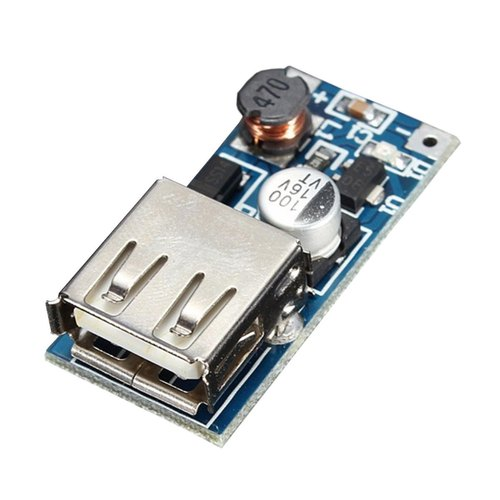
\includegraphics[width=0.4\linewidth]{Figures/dcdc_boost}
	\caption{Módulo comercial DC/DC en topología boost utilizado para alimentar la electrónica}
	\label{fig:dcdcboost}
\end{figure}\\
Su topología interna es \textit{boost} o elevador de tensión. En el HW del sistema, cumple la función de llevar la tensión variable del SC conectado a su entrada a una fija de 5 V. 
A su entrada admite tensiones variables desde 0,9 V hasta 5 V y puede otorgar hasta 500 miliamperes de corriente a la salida.

\subsection{Microcontrolador y firmware}
El MC es el ente encargado de ejecutar la lógica de negocios acorde a la tarea que debe cumplir el HW. En el mercado existe una amplia gama de fabricantes de placas de desarrollo que permiten acelerar la etapa de prototipado y validación de diseño.\\
La placa de desarrollo elegida para el prototipo fue la LoPy 4 producida por la firma Pycom y se presenta en la figura \ref{fig:lopy4} . En su interior alberga un ESP32, 8 Megabytes de memoria flash, transceptores de radio LoRa y 802.11 y un regulador de tensión.\\
\begin{figure}[h]
	\centering
	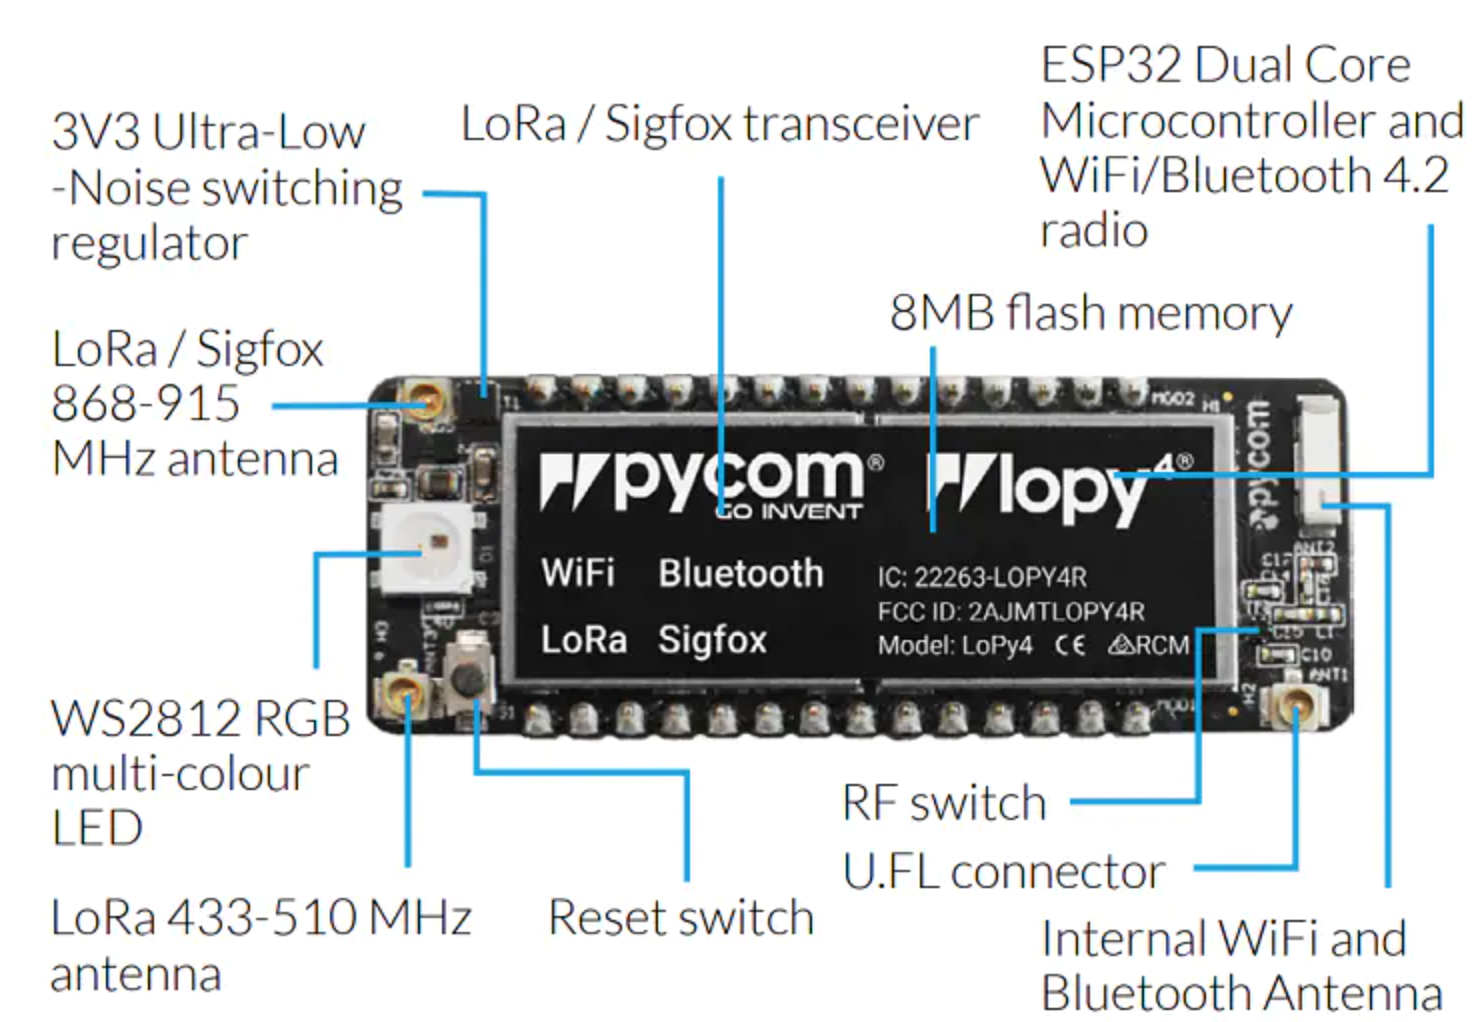
\includegraphics[width=0.7\linewidth]{Figures/lopy4}
	\caption{Placa de desarrollo LoPy 4 \citep{lopy4}}
	\label{fig:lopy4}
\end{figure}\\
El lenguaje de programación del LoPy4 es Micropython \citep{micropy}, un lenguaje de alto nivel lanzado por primera vez en el año 2014. Desde su lanzamiento y hasta la fecha de desarrollo de este trabajo, se presenta como una variante de Python atractiva para prototipar FW sobre microcontroladores utilizando el paradigma de programación orientada a objetos.\\


\section{Detalle del software}
\subsection{Red LoRaWAN}
LoRaWAN (Long Range Wide Area Network) es un protocolo de control de acceso al medio (MAC - \textit{Medium Acces Control}) definido por \textit{LoRa Aliance} \citep{lora_alliance}. Tiene por objeto permitir la conexión de nodos de baja potencia (generalmente alimentados a batería y sin capacidad de manejo de protocolos de enrutamiento por ejemplo TCP/IP) con aplicaciones finales conectadas a Internet mediante una conexión inalámbrica de largo alcance utilizando modulación LoRa.\\
Las puertas de enlace (GW - \textit{gateways}), están conectados al servidor central mediante conexiones IP (Internet Protocol) estándar cumpliendo la función de puente, es decir, convierte los paquetes de radiofrecuencia (RF) en paquetes IP y viceversa \ref{fig:arqlorawan}.\\
% TODO: \usepackage{graphicx} required
\begin{figure}[h]
	\centering
	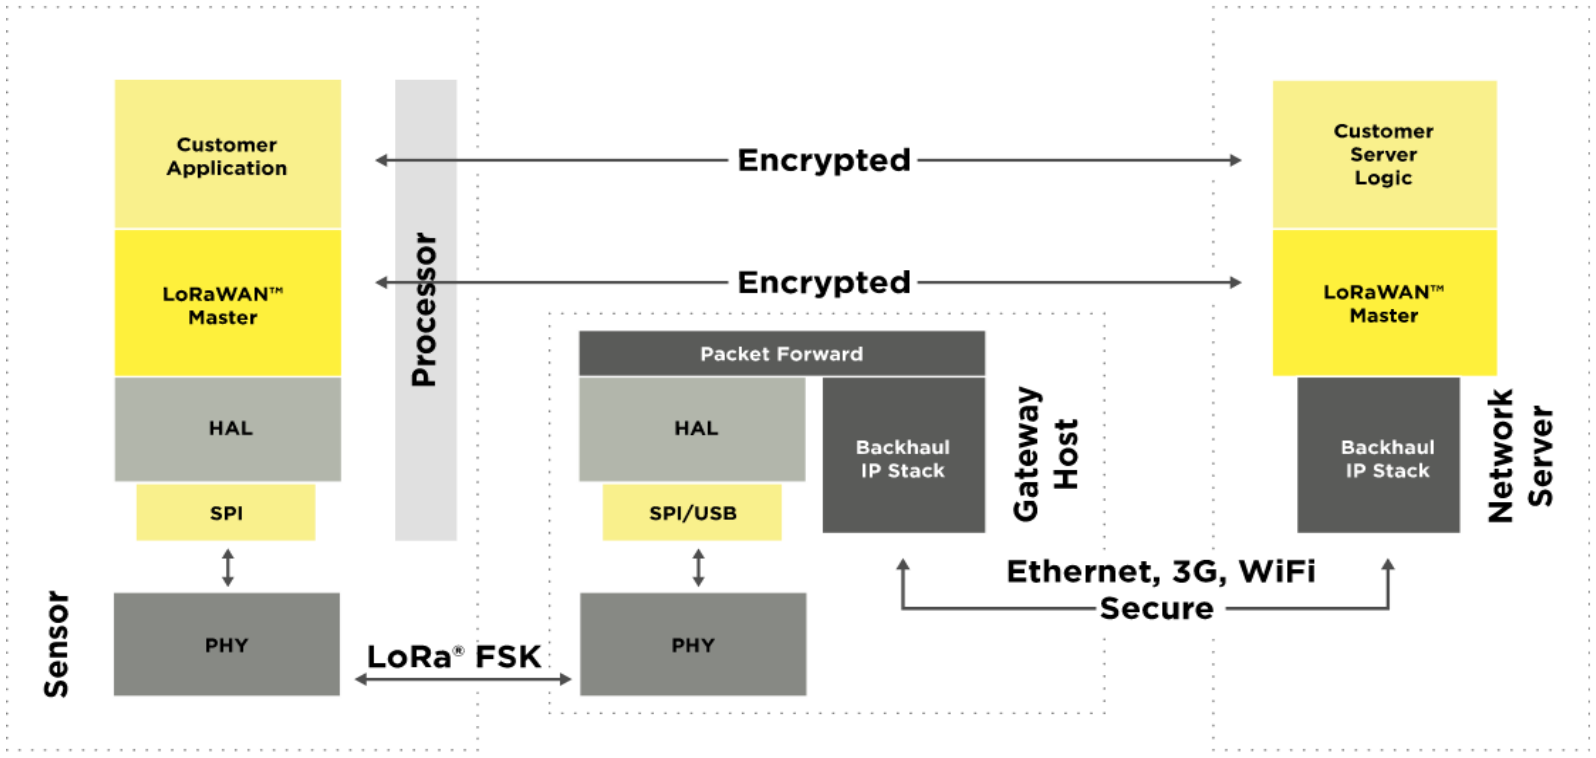
\includegraphics[width=0.9\linewidth]{Figures/arq_lorawan_2}
	\caption{Arquitectura de una red LoRaWAN y sus posibles integraciones con terceras partes \citep{lora_alliance}.}
	\label{fig:arqlorawan}
\end{figure}\\
El protocolo LoRaWAN no es un protocolo IP, por lo tanto, los paquetes del mismo necesitan de un enrutamiento y procesamiento correspondiente antes de ser entregados a la aplicación final.\\
La figura \ref{fig:sensor-gw-architecture-lora} presenta la topología tipo ``estrella de estrellas`` que adopta una red LoRaWAN. En ella los GW retransmiten los mensajes recibidos de los nodos finales hacia un servidor central. La comunicación inalámbrica entre nodos y GW aprovecha las características propias de la capa física, permitiendo así enlaces de un nodo hacia uno o más \textit{gateways}.\\
% TODO: \usepackage{graphicx} required
\begin{figure}[h]
	\centering
	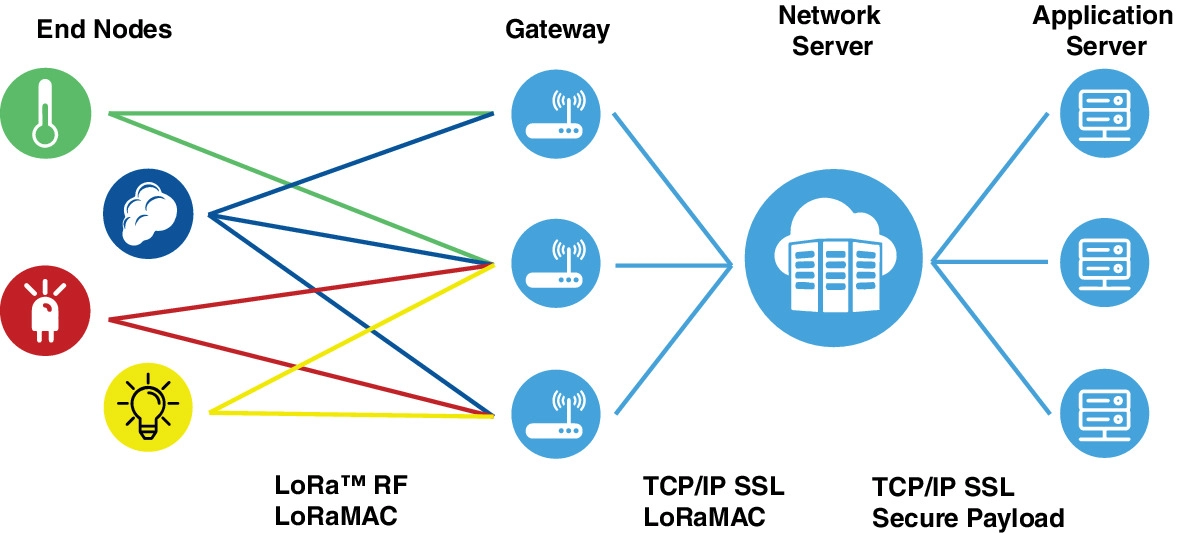
\includegraphics[width=0.9\linewidth]{Figures/sensor-gw-architecture-lora}
	\caption{Topología de una red LoRaWAN y la interacción entre los diferentes miembros \citep{lora_alliance}.}
	\label{fig:sensor-gw-architecture-lora}
\end{figure}

\subsection{Motor de base de datos}
Una base de datos (DB - \textit{Database}) almacena la información de manera ordenada en tablas o estructuras de datos. Las distintas aplicaciones pueden ejecutar consultas para solicitar la parte de esos datos que necesiten en ese momento.\\
Las bases de datos más utilizadas para aplicaciones web son las basadas en un modelo relacional, también conocidas como bases de datos SQL (Structured Query Language). Sin embargo, en años recientes se han popularizado las llamadas bases de datos NoSQL. Estas últimas están orientadas a documentos y almacena información de un mismo tipo en la forma de clave-valor.\\
Por su naturaleza, este proyecto parece indicado para utilizar NoSQL, ya que solo almacena registros de un tipo y no necesita crear relaciones complicadas entre distintas tablas de datos.\\
En principio se pensó en utilizar \textit{Elasticsearch} \citep{elasticsearch}, un servidor de búsqueda de texto basado en documentos JSON. Parecía el candidato ideal, ya que además de ser libre, se integraba perfectamente con Grafana, la herramienta para el desarrollo de la interfaz gráfica elegida \citep{grafana}.\\
Sin embargo, en las primeras pruebas llevadas a cabo se pudo apreciar que el consumo de memoria y procesamiento eran muy elevadas si se lo implementaba en un hardware modesto como las \textit{Raspberry Pi} \citep{raspi}. Finalmente se optó por utilizar MariaDB \citep{mariadb}, una base de datos del tipo SQL, también libre, con menos demanda de recursos y muy popular en aplicaciones web.\\

\subsection{Interfaz gráfica de usuario}
Una vez recuperados los datos de la red LoRaWAN y almacenados en la DB, una GUI presenta al usuario final del centro de operaciones los datos recolectados por cada nodo.\\
Una interfaz gráfica como la presentada en la figura \ref{fig:guirequeridaporelcliente}, se encarga de presentar al usuario final los últimos datos adquiridos por cada nodo. De esta manera, se puede identificar de manera simple mediante un punto verde o rojo sobre el mapa si la línea monitoreada presenta un problema.
% TODO: \usepackage{graphicx} required
\begin{figure}[h!]
	\centering
	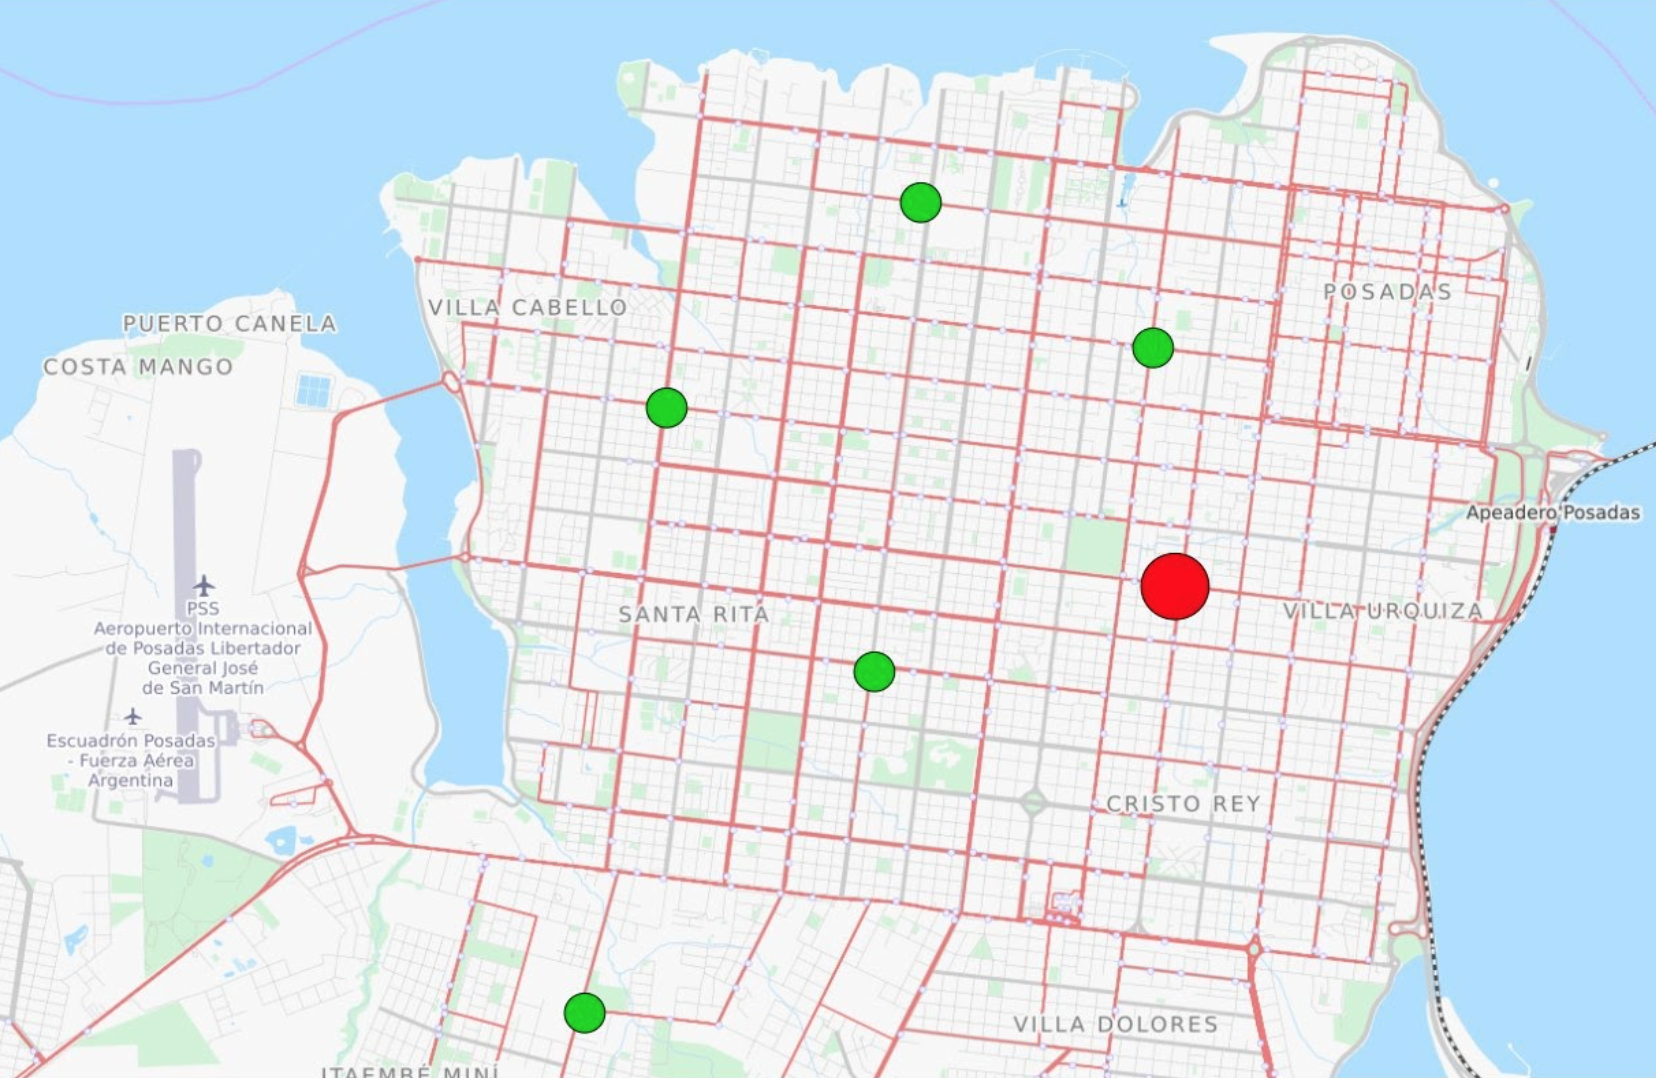
\includegraphics[width=0.7\linewidth]{Figures/GUI_requerida_por_el_cliente}
	\caption{Ejemplo de interfaz gráfica de usuario requerida por el cliente para presentar los últimos datos recuperados por cada nodo en la ciudad de Posadas, Misiones.}
	\label{fig:guirequeridaporelcliente}
\end{figure}\\
Para la presentación de la información se optó por Grafana, una aplicación web de código abierto para el análisis y visualización de datos, en especial datos temporales \citep{grafana}.\\
Grafana se adaptó muy bien a las necesidades del proyecto. Para mejorar aun más la experiencia del usuario se complementa con \textit{Worldmap Panel}, un \textit{plug in} que permite mostrar información temporal sobre un mapa. Esta información se presenta como círculos en las coordenadas donde se encuentra ubicado el nodo que genera la información.\\
 
	\chapter{Diseño e implementación} % Main chapter title

\label{Chapter3} % Change X to a consecutive number; for referencing this chapter elsewhere, use \ref{ChapterX}

\definecolor{mygreen}{rgb}{0,0.6,0}
\definecolor{mygray}{rgb}{0.5,0.5,0.5}
\definecolor{mymauve}{rgb}{0.58,0,0.82}

%%%%%%%%%%%%%%%%%%%%%%%%%%%%%%%%%%%%%%%%%%%%%%%%%%%%%%%%%%%%%%%%%%%%%%%%%%%%%
% parámetros para configurar el formato del código en los entornos lstlisting
%%%%%%%%%%%%%%%%%%%%%%%%%%%%%%%%%%%%%%%%%%%%%%%%%%%%%%%%%%%%%%%%%%%%%%%%%%%%%
\lstset{ %
  backgroundcolor=\color{white},   % choose the background color; you must add \usepackage{color} or \usepackage{xcolor}
  basicstyle=\footnotesize,        % the size of the fonts that are used for the code
  breakatwhitespace=false,         % sets if automatic breaks should only happen at whitespace
  breaklines=true,                 % sets automatic line breaking
  captionpos=b,                    % sets the caption-position to bottom
  commentstyle=\color{mygreen},    % comment style
  deletekeywords={...},            % if you want to delete keywords from the given language
  %escapeinside={\%*}{*)},          % if you want to add LaTeX within your code
  %extendedchars=true,              % lets you use non-ASCII characters; for 8-bits encodings only, does not work with UTF-8
  %frame=single,	                % adds a frame around the code
  keepspaces=true,                 % keeps spaces in text, useful for keeping indentation of code (possibly needs columns=flexible)
  keywordstyle=\color{blue},       % keyword style
  language=[ANSI]C,                % the language of the code
  %otherkeywords={*,...},           % if you want to add more keywords to the set
  numbers=left,                    % where to put the line-numbers; possible values are (none, left, right)
  numbersep=5pt,                   % how far the line-numbers are from the code
  numberstyle=\tiny\color{mygray}, % the style that is used for the line-numbers
  rulecolor=\color{black},         % if not set, the frame-color may be changed on line-breaks within not-black text (e.g. comments (green here))
  showspaces=false,                % show spaces everywhere adding particular underscores; it overrides 'showstringspaces'
  showstringspaces=false,          % underline spaces within strings only
  showtabs=false,                  % show tabs within strings adding particular underscores
  stepnumber=1,                    % the step between two line-numbers. If it's 1, each line will be numbered
  stringstyle=\color{mymauve},     % string literal style
  tabsize=2,	                   % sets default tabsize to 2 spaces
  title=\lstname,                  % show the filename of files included with \lstinputlisting; also try caption instead of title
  morecomment=[s]{/*}{*/}
}


%----------------------------------------------------------------------------------------
%	SECTION 1
%----------------------------------------------------------------------------------------
\section{Análisis del software}
 
La idea de esta sección es resaltar los problemas encontrados, los criterios utilizados y la justificación de las decisiones que se hayan tomado.

Se puede agregar código o pseudocódigo dentro de un entorno lstlisting con el siguiente código:

\begin{verbatim}
\begin{lstlisting}[caption= "un epígrafe descriptivo"]
	las líneas de código irían aquí...
\end{lstlisting}
\end{verbatim}

A modo de ejemplo:

\begin{lstlisting}[label=cod:vControl,caption=Pseudocódigo del lazo principal de control.]  % Start your code-block

#define MAX_SENSOR_NUMBER 3
#define MAX_ALARM_NUMBER  6
#define MAX_ACTUATOR_NUMBER 6

uint32_t sensorValue[MAX_SENSOR_NUMBER];		
FunctionalState alarmControl[MAX_ALARM_NUMBER];	//ENABLE or DISABLE
state_t alarmState[MAX_ALARM_NUMBER];						//ON or OFF
state_t actuatorState[MAX_ACTUATOR_NUMBER];			//ON or OFF

void vControl() {

	initGlobalVariables();
	
	period = 500 ms;
		
	while(1) {

		ticks = xTaskGetTickCount();
		
		updateSensors();
		
		updateAlarms();
		
		controlActuators();
		
		vTaskDelayUntil(&ticks, period);
	}
}
\end{lstlisting}




	% Chapter Template

\chapter{Ensayos y resultados} % Main chapter title

\label{Chapter4} % Change X to a consecutive number; for referencing this chapter elsewhere, use \ref{ChapterX}

%----------------------------------------------------------------------------------------
%	SECTION 1
%----------------------------------------------------------------------------------------

\section{PCB desarrollado}
\label{sec:pruebasHW}

\section{Medidor de valor RMS}\label{ensayo_medidor_rms}

\section{Circuito detector de cortes}

\section{Consumo en deep sleep}

\section{Autonom\'{i}a del supercapacitor}

\section{Ensayo end-to-end} 
	% Chapter Template

\chapter{Conclusiones} % Main chapter title

\label{Chapter5} % Change X to a consecutive number; for referencing this chapter elsewhere, use \ref{ChapterX}


%----------------------------------------------------------------------------------------

%----------------------------------------------------------------------------------------
%	SECTION 1
%----------------------------------------------------------------------------------------

\section{Conclusiones generales }
El sistema desarrollado, en concordancia con el objetivo general, conforma una herramienta económica para la prestadora del servicio de energía. Esta herramienta está diseñada para otorgar mayor granularidad de información sobre el estado de operación de las redes de distribución, sin implicar cambios significativos de infraestructura. Por otra parte, el análisis de la información suministrada permite identificar eventos recurrentes y evaluar sus posibles causas para poder delinear acciones correctivas y/o preventivas para mejorar la calidad de servicio.\\
Cumplimentando todos los requerimientos planteados por el cliente, y el tiempo planteado en la planificación, se ha logrado el desarrollo exitoso del sistema en todas sus partes: \textit{hardware}, \textit{firmware}, servicios de \textit{backend}; como así también su integración con la red LoRaWAN.\\
El uso de la red LPWAN de acceso público \textit{The Things Network} seleccionada para el trabajo, ha prestado servicios durante todo el desarrollo del proyecto sin solución de continuidad, demostrando así su buena cobertura y calidad de servicio a nivel global. A\'{u}n habiendo cambiado la localización geográfica de Europa a Sudamérica para realizar pruebas de laboratorio, la operación del sistema no se ha visto afectada en ningún aspecto.\\
El \textit{hardware} es capaz de convertir energía de corriente alterna proveniente del transformador de intensidad en otra de corriente continua y almacenarla. Los resultados del Capítulo 4, demuestran que el uso de circuitos de \textit{energy harvesting} en conjunto con tecnologías alternativas de acumulación en constante evolución como los supercapacitores, podrían ser sustitutos factibles de las baterías litio en aplicaciones autónomas que operen en régimen 24/7 y donde el rango de temperatura de operación necesaria sea mayor.\\
Las mediciones de valor RMS de corriente realizadas en el laboratorio, simulando la señal del TI con un generador de ondas y usando una carga de prueba presentadas en \ref{ensayo_medidor_rms}, demostraron la linealidad del circuito de medición dentro del rango de medición adoptado.\\
A partir de los ensayos de consumo en modo \textit{deep sleep} y autonomía de operación presentados en el capítulo \ref{Chapter4}, queda demostrado que el patrón \textit{power save loop} ha tenido un impacto significativamente positivo en la gestión de energía del nodo.\\
El tiempo total de propagación de datos desde el nodo \textit{in situ} hacia la red LoRaWAN, recuperación por los servicios de \textit{backend} y presentación en la interfaz gr\'{a}fica de usuario, es menor a 5 segundos. Este tiempo de propagación para el reporte de un problema, es considerado excelente en contraste con la situación actual en la provincia de Misiones.\\
Un conjunto de \textit{software} con abundante documentación tal como lo es LAMPP, ha ayudado a reducir el tiempo requerido para la puesta en funcionamiento de los servicios de \textit{backend} propios del proyecto y la integración con la red LoRaWAN a través de su API REST.\\
Durante la etapa de integración entre LoRaWAN y los servicios de \textit{backend}, fue destacable la importancia de la unificación del lenguaje de programación a Python en \'{e}ste proyecto. Además de su uso para el desarrollo del \textit{firmware}, se lo utilizó para implementar mockups que emulen los datos generados por el \textit{hardware}. Mediante el uso de esta técnica se pudo garantizar un flujo de desarrollo totalmente desacoplado de la necesidad de involucrar el \textit{hardware}, pero sí con una interacción constante entre servicios \textit{web} públicos y privados.\\


%----------------------------------------------------------------------------------------
%	SECTION 2
%----------------------------------------------------------------------------------------
\section{Trabajo a futuro}

Cumplidos los requerimientos y finalizado el trabajo propuesto, se han identificado las siguientes áreas de mejoras a futuro tanto en HW como SW:

\begin{itemize}
	\item Actualizar de manera inalámbrica el \textit{firmware} (OTA - \textit{Over The Air}): nuevas versiones del \textit{firmware} del microcontrolador aportarán nuevas funcionalidades, correcciones o mejoras sobre las ya existentes en nodos desplegados. Sin embargo, desarrollar esta funcionalidad es de alta prioridad antes de que el sistema llegue a una etapa de lanzamiento de producto. De esta manera, se prescindirá de la necesidad de intervenir físicamente cada nodo para actualizarlo.\\
	\item Modularizar el PCB para realizar mediciones de 3 fases: dado que los sistemas de distribución son trifásicos, el HW deberá también permitir realizar mediciones de corrientes sobre las 3 fases del sistema. Para lograr esto se debería proponer una modularización de la etapa de medición de valor RMS de corriente.\\
	\item Integrar servicios de mensajería instantánea: si bien la GUI permite de manera rápida identificar sobre un mapa el punto geográfico donde la red presenta un problema o su estado actual de operación, contar con una aplicación similar para dispositivos móviles será de utilidad para el personal encargado de cumplir horarios de guardia.\\
	
\end{itemize}

 
\end{verbatim}

Los apéndices también deben escribirse en archivos .tex separados, que se deben ubicar dentro de la carpeta \emph{Appendices}. Los apéndices vienen comentados por defecto con el caracter \code{\%} y para incluirlos simplemente se debe eliminar dicho caracter.

Finalmente, se encuentra el código para incluir la bibliografía en el documento final.  Este código tampoco debe modificarse. La metodología para trabajar las referencias bibliográficas se desarrolla en la sección \ref{sec:biblio}.
%----------------------------------------------------------------------------------------

\section{Bibliografía}
\label{sec:biblio}

Las opciones de formato de la bibliografía se controlan a través del paquete de latex \option{biblatex} que se incluye en la memoria en el archivo memoria.tex.  Estas opciones determinan cómo se generan las citas bibliográficas en el cuerpo del documento y cómo se genera la bibliografía al final de la memoria.

En el preámbulo se puede encontrar el código que incluye el paquete biblatex, que no requiere ninguna modificación del usuario de la plantilla, y que contiene las siguientes opciones:

\begin{lstlisting}
\usepackage[backend=bibtex,
	natbib=true, 
	style=numeric, 
	sorting=none]
{biblatex}
\end{lstlisting}

En el archivo \file{reference.bib} se encuentran las referencias bibliográficas que se pueden citar en el documento.  Para incorporar una nueva cita al documento lo primero es agregarla en este archivo con todos los campos necesario.  Todas las entradas bibliográficas comienzan con $@$ y una palabra que define el formato de la entrada.  Para cada formato existen campos obligatorios que deben completarse. No importa el orden en que las entradas estén definidas en el archivo .bib.  Tampoco es importante el orden en que estén definidos los campos de una entrada bibliográfica. A continuación se muestran algunos ejemplos:

\begin{lstlisting}
@ARTICLE{ARTICLE:1,
    AUTHOR="John Doe",
    TITLE="Title",
    JOURNAL="Journal",
    YEAR="2017",
}
\end{lstlisting}


\begin{lstlisting}
@BOOK{BOOK:1,
    AUTHOR="John Doe",
    TITLE="The Book without Title",
    PUBLISHER="Dummy Publisher",
    YEAR="2100",
}
\end{lstlisting}


\begin{lstlisting}
@INBOOK{BOOK:2,
    AUTHOR="John Doe",
    TITLE="The Book without Title",
    PUBLISHER="Dummy Publisher",
    YEAR="2100",
    PAGES="100-200",
}
\end{lstlisting}


\begin{lstlisting}
@MISC{WEBSITE:1,
    HOWPUBLISHED = "\url{http://example.com}",
    AUTHOR = "Intel",
    TITLE = "Example Website",
    MONTH = "12",
    YEAR = "1988",
    URLDATE = {2012-11-26}
}
\end{lstlisting}

Se debe notar que los nombres \emph{ARTICLE:1}, \emph{BOOK:1}, \emph{BOOK:2} y \emph{WEBSITE:1} son nombres de fantasía que le sirve al autor del documento para identificar la entrada. En este sentido, se podrían reemplazar por cualquier otro nombre.  Tampoco es necesario poner : seguido de un número, en los ejemplos sólo se incluye como un posible estilo para identificar las entradas.

La entradas se citan en el documento con el comando: 

\begin{verbatim}
\citep{nombre_de_la_entrada}
\end{verbatim}

Y cuando se usan, se muestran así: \citep{ARTICLE:1}, \citep{BOOK:1}, \citep{BOOK:2}, \citep{WEBSITE:1}.  Notar cómo se conforma la sección Bibliografía al final del documento. 

	\chapter{Introducción específica} % Main chapter title
\label{Chapter2}
%----------------------------------------------------------------------------------------
%	SECTION 1
%----------------------------------------------------------------------------------------
En este capítulo se presentan los requerimientos acordados con el cliente y los recursos de \textit{hardware} (HW) y \textit{software} (SW) utilizados para el desarrollo del trabajo. Se describen en las partes implementadas del HW, los servicios integrados de \textit{backend} (BES) y solamente algunos aspectos relevantes del \textit{firmware} (FW) que interactúa con el HW. En el capítulo 3 se abarca la lógica de negocios implementada en el FW del microcontrolador.\\
\section{Requerimientos acordados con el cliente}
\label{sec:requerimientos}
\begin{enumerate}
	\item Grupo de requerimientos asociados con hardware
	\begin{enumerate}
		\item El dispositivo deberá ser de tipo \textit{plug and play}.
		\item El circuito impreso no deberá ocupar un volumen mayor a 10x10x5 cm.
		\item Basarse en un microcontrolador ESP32 y disponer de:
		\begin{enumerate}%[label*=\arabic*.]
			\item 4 entradas analógicas.
			\item 3 salidas digitales.
			\item Unidad UART.
			\item Integrar un módulo de comunicaciones LoRa.
		\end{enumerate}
		\item Deberá tener al menos 12 horas de autonomía de funcionamiento.
		\item Bajo consumo en modo ocioso: el consumo del hardware en total, no deberá superar los 5 mA cuando no está midiendo ni transmitiendo.
		\item El circuito elevador de tensión DC-DC deberá:
		\begin{enumerate}%[label*=\arabic*.]
			\item Funcionar con tensiones menores a 2V en la entrada.
			\item Otorgar 5 Volts a la salida.
			\item Ser capaz de otorgar 300 miliamperes a la salida.
		\end{enumerate}
		\item El transformador de corriente (TI) debe:
		\begin{enumerate}%[label*=\arabic*.]
			\item Ser de tipo núcleo partido.
			\item Admitir 100 Amperes de corriente en el circuito primario y un máximo 5 Amperes en el circuito secundario.
		\end{enumerate}
		\item \label{req_relay} El relay encargado de cambiar el modo de operación debe:
		\begin{enumerate}%[label*=\arabic*.]
			\item Ser de tipo doble inversor sin retención.
			\item Su bobina debe poder energizarse con 5V o menos.
			\item Soportar al menos 5 Amperes de corriente por los contactos.
		\end{enumerate} 
		\item Debe funcionar de manera independiente a la frecuencia de operación de la red 50/60 Hz.
		\item Debe funcionar de manera independiente a la tensión de fase del sistema de distribución 110/220 Voltios.
	\end{enumerate}
	\item Grupo de requerimientos asociados con el firmware
	\begin{enumerate}
		\item Debe manejar un módulo de comunicación LoRa y protocolo LoRaWAN.
		\item Deberá tener un porcentaje de cobertura de tests unitarios del 60\% como mínimo.
		\item Antes configurarse en modo ocioso, debe desenergizar la etapa de medición de corriente y el módulo de comunicaciones con el objeto de ahorrar energía.
	\end{enumerate}
	
	\item Grupo de requerimientos asociados con los servicios de backend (BES)
	\label{requerimientos_backend}
	\begin{enumerate}
		\item Todos los servicios deben poder correr en una Raspberry Pi 3.
		\item El \textit{software} de los BES se desarrollará en lenguaje Python.
		\item Recuperar los datos de la red LoRaWAN.\label{requerimiento_LORAWAN}
		\item Almacenar los datos en una tabla de MySQL.
		\item (GUI - \textit{Graphical User Interface}) basada en Grafana.
	\end{enumerate}
	
	\item Grupo de requerimientos asociados con ensayos de integración y \textit{end-to-end}
	\begin{enumerate}
		\item El banco de ensayos de \textit{hardware} debe contar con una carga fantasma de al menos 10 Amperes y permitir realizar interrupciones de corriente de manera programada mediante una computadora adicional tipo Raspberry Pi o de manera manual.
		\item Los BES deben estar operativos al momento de realizar los ensayos.
		\item Contar con un gateway de acceso a una red LoRaWAN como por ejemplo \textit{The Things Network}.
	\end{enumerate}
\end{enumerate}


\section{Diagrama de bloques general del sistema implementado}
El diagrama de bloques del HW a instalar \textit{in situ} es presentado en la figura \ref{fig:diagramadebloquesdelhw} y consta de cuatro bloques:
% TODO: \usepackage{graphicx} required
\begin{figure}[h!]
	\centering
	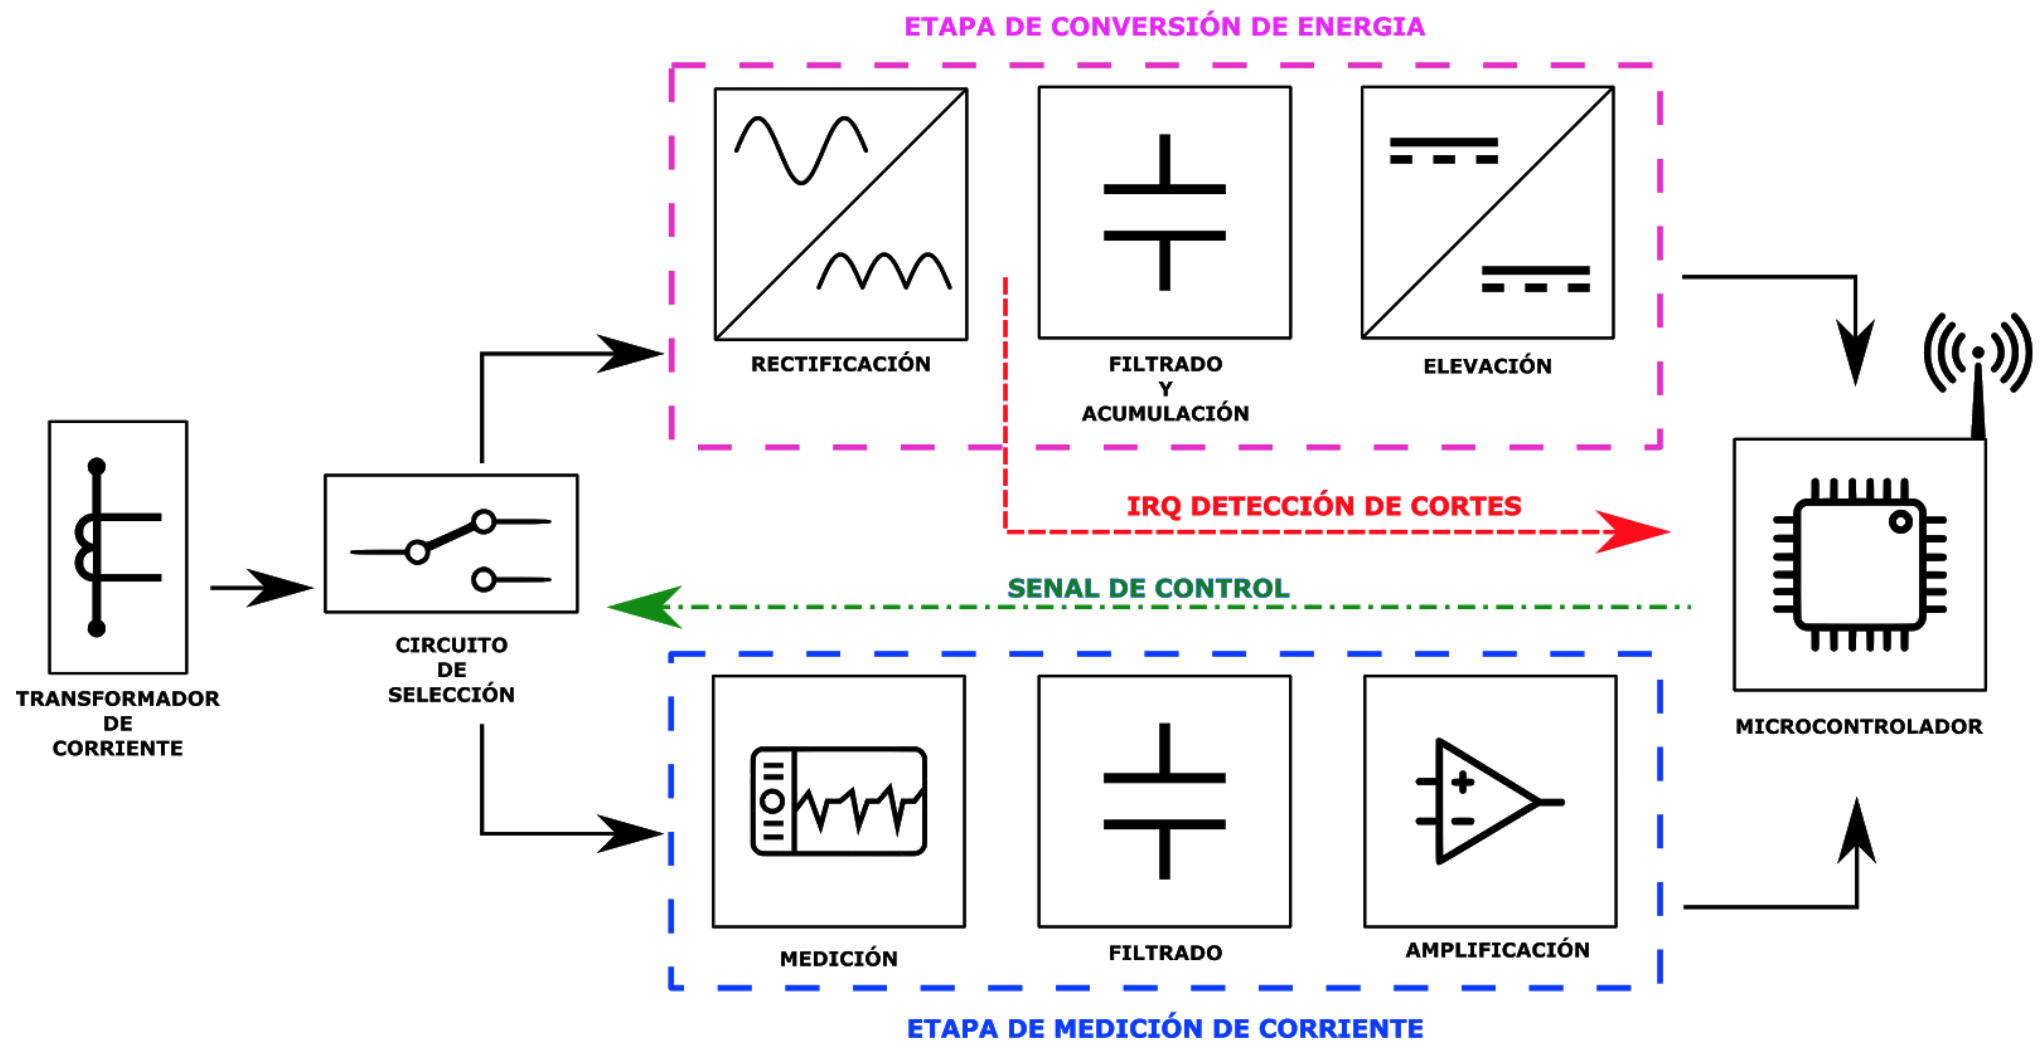
\includegraphics[width=0.7\linewidth]{Figures/diagrama_de_bloques_del_HW}
	\caption{Diagrama de bloques del HW para el nodo a instalar \textit{in situ}}
	\label{fig:diagramadebloquesdelhw}
\end{figure}
\begin{enumerate}
	\item Circuito de selección de modo: un relay (RL) y su circuito de mando controlarán a que etapa del nodo se conectarán los terminales del TI.
	\item Etapa de rectificación, acumulación de energía y elevación de tensión: compuesta por rectificador de onda completa, una etapa de filtrado y acumulación y un circuito elevador de tensión.
	\item Etapa de medición de valor RMS de corriente: un chip dedicado toma la señal de tensión generada en bornes del resistor shunt y calcula el valor RMS. A su salida entrega un valor proporcional de tensión DC.
	\item Microcontrolador (MC): ejecuta la lógica de negocios que rige el comportamiento del nodo, digitalizar mediciones y transmitir datos a la red LoRaWAN.
\end{enumerate}
Por otro lado, el sistema también implicó el desarrollo y puesta en funcionamiento de un conjunto de servicios de \textit{backend} (BES) propios del proyecto que cumplen las funciones de:
\begin{itemize}
	\item Recuperación de datos de la red LoRaWAN.
	\item Almacenamiento en una base de datos (DB).
	\item Presentación de los datos al usuario final mediante una interfaz gráfica de usuario (GUI).
\end{itemize}

El requisito \ref{requerimiento_LORAWAN} impuso el uso de una red LoRaWAN como columna vertebral para la transmisión de datos generados por los nodos. Para cumplirlo se adoptó la arquitectura presentada en la figura \ref{fig:diagramadebloquesdebes}.\\
% TODO: \usepackage{graphicx} required
\begin{figure}[h!]
	\centering
	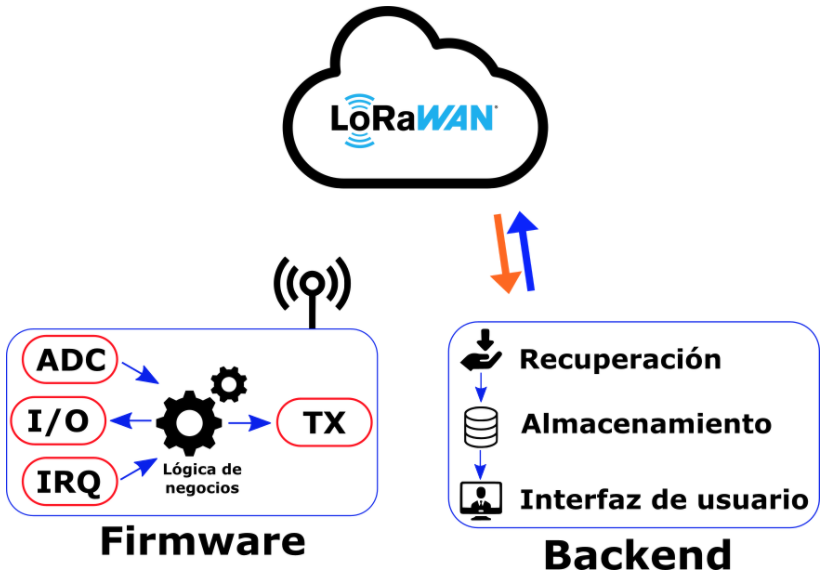
\includegraphics[width=0.6\linewidth]{Figures/diagrama_de_bloques_de_BES}
	\caption{Diagrama de bloques del FW implementado en el MC y su interacción con la red LoRaWAN y los BES privados del sistema.}
	\label{fig:diagramadebloquesdebes}
\end{figure}\\
Las mediciones son tomadas por el HW y transmitidas hacia la red LoRaWAN para luego interactuar con los BES privados que se encargan de recuperar, almacenar y presentar los datos al usuario final.\\


\section{Detalle del hardware}
\subsection{Transformador de corriente}
Un transformador de corriente o intensidad (TI) es un dispositivo de medición utilizado para producir en su devanado secundario una corriente diferente y proporcional a la que circula por su devanado primario.\\
El principio de operación de un TI no es diferente al de un transformador de potencia convencional. A diferencia de uno de potencia, el devanado primario puede ser de una sola vuelta sobre un núcleo ferromagnético como se ve en la figura \ref{fig:dibujomedicionti}. El devanado secundario suele tener un número mayor de vueltas alrededor del núcleo y depende de que tanto se debe reducir la corriente.\\
% TODO: \usepackage{graphicx} required
\begin{figure}[h!]
	\centering
	\includegraphics[width=0.5\linewidth]{Figures/dibujo_medicion_TI}
	\caption{Circuito de medición indirecta de corriente mediante un TI.\citep{hioki}}
	\label{fig:dibujomedicionti}
\end{figure}\\
Muchos TI tienen una relación estándar de 5 Amperes en el secundario, por ejemplo un TI 200/5 significa que cuando por el primario fluyen 200 amperes en el secundario solo fluyen 5. Es decir, el TI tiene una relación de transformación de corriente N de 40 veces.\\
Mediante esta técnica, pequeños instrumentos pueden monitorear grandes valores de corriente manteniendo una distancia segura de las líneas de alta tensión.


\subsection{Circuito de selección}
A partir del lineamiento de que el TI debe estar conectado por defecto a la entrada del rectificador y al resistor shunt al energizarse la bobina del RL, el número y la disposición de los contactos fue un factor relevante al momento de elegir la mejor opción. La variante comercial que cumplió con los requisitos \ref{req_relay} es la producida por la firma Hongfa modelo HF115F/005-2ZS4A presentada en la figura \ref{fig:relay}.
\begin{figure}[h!]
    \centering
	\begin{subfigure}[b]{0.3\textwidth}
		\centering
		\includegraphics[width=.65\textwidth]{./Figures/relay_pinout}
		\caption{}
		\label{fig:relay_pinout}
	\end{subfigure}
    \centering
	\begin{subfigure}[b]{0.3\textwidth}
		\centering
		\includegraphics[width=.65\textwidth]{./Figures/relay_encapsulado}
		\caption{}
		\label{fig:relay_encapsulado}
	\end{subfigure}
	\caption{Pinout del relay HF115F/005-2ZS4A (izquireda) y su encapsulado (derecha). Imágenes tomadas de \citep{datasheet_relay}}
	\label{fig:relay}
\end{figure}

\subsection{Conversión de energía}
Para obtener una tensión continua a partir de una alterna generada por el TI, es necesario implementar un puente rectificador de onda completa.\\
En la actualidad la mayoría de los circuitos rectificadores de onda completa se basan en diodos de silicio de bajo costo. Sin embargo, un diodo de silicio posee una caída de tensión típica de 0,7 V. Esta caída de tensión se traduce en pérdidas por efecto Joule y es relevante en dispositivos donde la conversión, acumulación y gestión de energía es crítica. Por lo tanto, se desea maximizar la transferencia de tensión y potencia entre entrada y salida del puente rectificador.\\
Yilmaz \citep{Yilmaz} analiza técnicas de rectificación de onda completa con diferentes tipos de diodos, como así también un arreglo de transistores MOSFET pasivo y activo. Las caídas de tensión simuladas entre la entrada y salida entre un puente rectificador de diodos de silicio y uno pasivo basado en MOSFETs se comparan en la figura \ref{fig:comparacion_diodos_vs_MOSFET}.\\

\begin{figure}[h!]
	\begin{subfigure}{.5\textwidth}
		\centering
		% include first image
		\includegraphics[width=.8\linewidth]{Figures/YILMAZ_silicon_diode_rectifier}  
		\caption{Rectificador basado en diodos de silicio}
		\label{fig:rect_diodos}
	\end{subfigure}
	\begin{subfigure}{.5\textwidth}
		\centering
		% include second image
		\includegraphics[width=.8\linewidth]{Figures/onda_silicon_rectifier}  
		\caption{Caída de tensión generada por el rectificador de la figura \ref{fig:rect_diodos}}
		\label{fig:onda_rectificador_diodos}
	\end{subfigure}
	\newline
	\begin{subfigure}{.5\textwidth}
		\centering
		% include third image
		\includegraphics[width=.8\linewidth]{Figures/YILMAZ_passive_MOSFET_rectifier}  
		\caption{Rectificador basado en transistores MOSFET}
		\label{fig:rect_MOSFET}
	\end{subfigure}
	\begin{subfigure}{.5\textwidth}
		\centering
		% include fourth image
		\includegraphics[width=.8\linewidth]{Figures/onda_passive_mosfet_rectifier}  
		\caption{Caída de tensión generada por el rectificador de la figura \ref{fig:rect_MOSFET}}
		\label{fig:onda_rectificador_MOSFET}
	\end{subfigure}
	\caption{Simulación de rectificadores basados en diodos y MOSFET. Imágenes tomadas de: \citep{Yilmaz}}
	\label{fig:comparacion_diodos_vs_MOSFET}
\end{figure}
Al comparar las simulaciones expuestas en las figuras \ref{fig:onda_rectificador_diodos} y \ref{fig:onda_rectificador_MOSFET} se aprecia que la caída de tensión generada por el rectificador basado en MOSFET al entrar en conducción es menor que uno hecho con diodos, por lo tanto también la potencia disipada en forma de calor.\\

\subsection{Supercapacitor como acumulador de energía}
La decisión de optar por un banco de supercapacitores (SC) como reemplazo total de una batería, se basa principalmente en el entorno donde operará el nodo HW. Diferencias entre una batería y un SC de interés para este proyecto, se plasman en la tabla \ref{tab:batteria_vs_supercap}.\\
Datos meteorológicos de la provincia de Misiones presentados en \citep{historico_temperaturas}, acusan temperaturas por encima de 30 C durante el periodo de septiembre a marzo. A diferencia de un SC que posee un rango de temperaturas de operación desde los -40 C hasta 70 C \citep{datasheet_supercap}, condiciones por encima de 35 grados son nocivas para una batería y generan el deterioro prematuro de sus componentes\citep{MA2018653}.\\
%\begin{verbatim}
\begin{table}[h]
	\centering
	\caption{Comparativa entre una batería y un supercapacitor para este proyecto}
	\begin{tabular}{lcc} 
		\hline
		\multicolumn{1}{c}{}                                                  & Batería         & Supercapacitor                                                                         \\ 
		\hline
		\begin{tabular}[c]{@{}l@{}}Densidad de \\energía (Wh/Kg)\end{tabular} & 265             & 3,9                                                                                    \\
		\begin{tabular}[c]{@{}l@{}}Rango de \\temperatura (C)\end{tabular}    & 15 a 35         & -40 a 70                                                                               \\
		Gestión de carga                                                      & V o I constante & \begin{tabular}[c]{@{}c@{}}Determinado por un\\circuito RC serie \citep{ceraolo2014fundamentals}\end{tabular}  \\
		\hline
	\end{tabular}
	\label{tab:batteria_vs_supercap}
\end{table}\\
%\end{verbatim}
Es importante remarcar que la densidad de energía que pueden almacenar también es diferente, una batería tiene una densidad de energía 60 veces mayor que un SC. Sin embargo, para esta aplicación puntual no representó un factor importante a la hora de elegir el acumulador.\\
Por último, el ciclo de carga es más complejo en el caso de una batería. Las etapas de su curva de carga deben ser respetados según sean a corriente o tensión constante. Esto trae acarreado implementar una electrónica adicional encargada de gestionar estos 2 parámetros. En un capacitor, la curva de carga está definida por un circuito RC serie \citep{ceraolo2014fundamentals}.\\ 

\subsection{Elevación de tensión mediante un conversor DC/DC }
Para proveer al MC, y el resto de la electrónica asociada de una tensión DC fija y constante, se ha optado por emplear un módulo comercial DC/DC ya existente en el mercado y es presentado en la figura \ref{fig:dcdcboost}.\\
% TODO: \usepackage{graphicx} required
\begin{figure}[h!]
	\centering
	\includegraphics[width=0.4\linewidth]{Figures/dcdc_boost}
	\caption{Módulo comercial DC/DC en topología boost utilizado para alimentar la electrónica}
	\label{fig:dcdcboost}
\end{figure}\\
Su topología interna es \textit{boost} o elevador de tensión. En el HW del sistema, cumple la función de llevar la tensión variable del SC conectado a su entrada a una fija de 5 V. 
A su entrada admite tensiones variables desde 0,9 V hasta 5 V y puede otorgar hasta 500 miliamperes de corriente a la salida.

\subsection{Microcontrolador y firmware}
El MC es el ente encargado de ejecutar la lógica de negocios acorde a la tarea que debe cumplir el HW. En el mercado existe una amplia gama de fabricantes de placas de desarrollo que permiten acelerar la etapa de prototipado y validación de diseño.\\
La placa de desarrollo elegida para el prototipo fue la LoPy 4 producida por la firma Pycom y se presenta en la figura \ref{fig:lopy4} . En su interior alberga un ESP32, 8 Megabytes de memoria flash, transceptores de radio LoRa y 802.11 y un regulador de tensión.\\
\begin{figure}[h]
	\centering
	\includegraphics[width=0.7\linewidth]{Figures/lopy4}
	\caption{Placa de desarrollo LoPy 4 \citep{lopy4}}
	\label{fig:lopy4}
\end{figure}\\
El lenguaje de programación del LoPy4 es Micropython \citep{micropy}, un lenguaje de alto nivel lanzado por primera vez en el año 2014. Desde su lanzamiento y hasta la fecha de desarrollo de este trabajo, se presenta como una variante de Python atractiva para prototipar FW sobre microcontroladores utilizando el paradigma de programación orientada a objetos.\\


\section{Detalle del software}
\subsection{Red LoRaWAN}
LoRaWAN (Long Range Wide Area Network) es un protocolo de control de acceso al medio (MAC - \textit{Medium Acces Control}) definido por \textit{LoRa Aliance} \citep{lora_alliance}. Tiene por objeto permitir la conexión de nodos de baja potencia (generalmente alimentados a batería y sin capacidad de manejo de protocolos de enrutamiento por ejemplo TCP/IP) con aplicaciones finales conectadas a Internet mediante una conexión inalámbrica de largo alcance utilizando modulación LoRa.\\
Las puertas de enlace (GW - \textit{gateways}), están conectados al servidor central mediante conexiones IP (Internet Protocol) estándar cumpliendo la función de puente, es decir, convierte los paquetes de radiofrecuencia (RF) en paquetes IP y viceversa \ref{fig:arqlorawan}.\\
% TODO: \usepackage{graphicx} required
\begin{figure}[h]
	\centering
	\includegraphics[width=0.9\linewidth]{Figures/arq_lorawan_2}
	\caption{Arquitectura de una red LoRaWAN y sus posibles integraciones con terceras partes \citep{lora_alliance}.}
	\label{fig:arqlorawan}
\end{figure}\\
El protocolo LoRaWAN no es un protocolo IP, por lo tanto, los paquetes del mismo necesitan de un enrutamiento y procesamiento correspondiente antes de ser entregados a la aplicación final.\\
La figura \ref{fig:sensor-gw-architecture-lora} presenta la topología tipo ``estrella de estrellas`` que adopta una red LoRaWAN. En ella los GW retransmiten los mensajes recibidos de los nodos finales hacia un servidor central. La comunicación inalámbrica entre nodos y GW aprovecha las características propias de la capa física, permitiendo así enlaces de un nodo hacia uno o más \textit{gateways}.\\
% TODO: \usepackage{graphicx} required
\begin{figure}[h]
	\centering
	\includegraphics[width=0.9\linewidth]{Figures/sensor-gw-architecture-lora}
	\caption{Topología de una red LoRaWAN y la interacción entre los diferentes miembros \citep{lora_alliance}.}
	\label{fig:sensor-gw-architecture-lora}
\end{figure}

\subsection{Motor de base de datos}
Una base de datos (DB - \textit{Database}) almacena la información de manera ordenada en tablas o estructuras de datos. Las distintas aplicaciones pueden ejecutar consultas para solicitar la parte de esos datos que necesiten en ese momento.\\
Las bases de datos más utilizadas para aplicaciones web son las basadas en un modelo relacional, también conocidas como bases de datos SQL (Structured Query Language). Sin embargo, en años recientes se han popularizado las llamadas bases de datos NoSQL. Estas últimas están orientadas a documentos y almacena información de un mismo tipo en la forma de clave-valor.\\
Por su naturaleza, este proyecto parece indicado para utilizar NoSQL, ya que solo almacena registros de un tipo y no necesita crear relaciones complicadas entre distintas tablas de datos.\\
En principio se pensó en utilizar \textit{Elasticsearch} \citep{elasticsearch}, un servidor de búsqueda de texto basado en documentos JSON. Parecía el candidato ideal, ya que además de ser libre, se integraba perfectamente con Grafana, la herramienta para el desarrollo de la interfaz gráfica elegida \citep{grafana}.\\
Sin embargo, en las primeras pruebas llevadas a cabo se pudo apreciar que el consumo de memoria y procesamiento eran muy elevadas si se lo implementaba en un hardware modesto como las \textit{Raspberry Pi} \citep{raspi}. Finalmente se optó por utilizar MariaDB \citep{mariadb}, una base de datos del tipo SQL, también libre, con menos demanda de recursos y muy popular en aplicaciones web.\\

\subsection{Interfaz gráfica de usuario}
Una vez recuperados los datos de la red LoRaWAN y almacenados en la DB, una GUI presenta al usuario final del centro de operaciones los datos recolectados por cada nodo.\\
Una interfaz gráfica como la presentada en la figura \ref{fig:guirequeridaporelcliente}, se encarga de presentar al usuario final los últimos datos adquiridos por cada nodo. De esta manera, se puede identificar de manera simple mediante un punto verde o rojo sobre el mapa si la línea monitoreada presenta un problema.
% TODO: \usepackage{graphicx} required
\begin{figure}[h!]
	\centering
	\includegraphics[width=0.7\linewidth]{Figures/GUI_requerida_por_el_cliente}
	\caption{Ejemplo de interfaz gráfica de usuario requerida por el cliente para presentar los últimos datos recuperados por cada nodo en la ciudad de Posadas, Misiones.}
	\label{fig:guirequeridaporelcliente}
\end{figure}\\
Para la presentación de la información se optó por Grafana, una aplicación web de código abierto para el análisis y visualización de datos, en especial datos temporales \citep{grafana}.\\
Grafana se adaptó muy bien a las necesidades del proyecto. Para mejorar aun más la experiencia del usuario se complementa con \textit{Worldmap Panel}, un \textit{plug in} que permite mostrar información temporal sobre un mapa. Esta información se presenta como círculos en las coordenadas donde se encuentra ubicado el nodo que genera la información.\\
 
	\chapter{Diseño e implementación} % Main chapter title

\label{Chapter3} % Change X to a consecutive number; for referencing this chapter elsewhere, use \ref{ChapterX}

\definecolor{mygreen}{rgb}{0,0.6,0}
\definecolor{mygray}{rgb}{0.5,0.5,0.5}
\definecolor{mymauve}{rgb}{0.58,0,0.82}

%%%%%%%%%%%%%%%%%%%%%%%%%%%%%%%%%%%%%%%%%%%%%%%%%%%%%%%%%%%%%%%%%%%%%%%%%%%%%
% parámetros para configurar el formato del código en los entornos lstlisting
%%%%%%%%%%%%%%%%%%%%%%%%%%%%%%%%%%%%%%%%%%%%%%%%%%%%%%%%%%%%%%%%%%%%%%%%%%%%%
\lstset{ %
  backgroundcolor=\color{white},   % choose the background color; you must add \usepackage{color} or \usepackage{xcolor}
  basicstyle=\footnotesize,        % the size of the fonts that are used for the code
  breakatwhitespace=false,         % sets if automatic breaks should only happen at whitespace
  breaklines=true,                 % sets automatic line breaking
  captionpos=b,                    % sets the caption-position to bottom
  commentstyle=\color{mygreen},    % comment style
  deletekeywords={...},            % if you want to delete keywords from the given language
  %escapeinside={\%*}{*)},          % if you want to add LaTeX within your code
  %extendedchars=true,              % lets you use non-ASCII characters; for 8-bits encodings only, does not work with UTF-8
  %frame=single,	                % adds a frame around the code
  keepspaces=true,                 % keeps spaces in text, useful for keeping indentation of code (possibly needs columns=flexible)
  keywordstyle=\color{blue},       % keyword style
  language=[ANSI]C,                % the language of the code
  %otherkeywords={*,...},           % if you want to add more keywords to the set
  numbers=left,                    % where to put the line-numbers; possible values are (none, left, right)
  numbersep=5pt,                   % how far the line-numbers are from the code
  numberstyle=\tiny\color{mygray}, % the style that is used for the line-numbers
  rulecolor=\color{black},         % if not set, the frame-color may be changed on line-breaks within not-black text (e.g. comments (green here))
  showspaces=false,                % show spaces everywhere adding particular underscores; it overrides 'showstringspaces'
  showstringspaces=false,          % underline spaces within strings only
  showtabs=false,                  % show tabs within strings adding particular underscores
  stepnumber=1,                    % the step between two line-numbers. If it's 1, each line will be numbered
  stringstyle=\color{mymauve},     % string literal style
  tabsize=2,	                   % sets default tabsize to 2 spaces
  title=\lstname,                  % show the filename of files included with \lstinputlisting; also try caption instead of title
  morecomment=[s]{/*}{*/}
}


%----------------------------------------------------------------------------------------
%	SECTION 1
%----------------------------------------------------------------------------------------
\section{Análisis del software}
 
La idea de esta sección es resaltar los problemas encontrados, los criterios utilizados y la justificación de las decisiones que se hayan tomado.

Se puede agregar código o pseudocódigo dentro de un entorno lstlisting con el siguiente código:

\begin{verbatim}
\begin{lstlisting}[caption= "un epígrafe descriptivo"]
	las líneas de código irían aquí...
\end{lstlisting}
\end{verbatim}

A modo de ejemplo:

\begin{lstlisting}[label=cod:vControl,caption=Pseudocódigo del lazo principal de control.]  % Start your code-block

#define MAX_SENSOR_NUMBER 3
#define MAX_ALARM_NUMBER  6
#define MAX_ACTUATOR_NUMBER 6

uint32_t sensorValue[MAX_SENSOR_NUMBER];		
FunctionalState alarmControl[MAX_ALARM_NUMBER];	//ENABLE or DISABLE
state_t alarmState[MAX_ALARM_NUMBER];						//ON or OFF
state_t actuatorState[MAX_ACTUATOR_NUMBER];			//ON or OFF

void vControl() {

	initGlobalVariables();
	
	period = 500 ms;
		
	while(1) {

		ticks = xTaskGetTickCount();
		
		updateSensors();
		
		updateAlarms();
		
		controlActuators();
		
		vTaskDelayUntil(&ticks, period);
	}
}
\end{lstlisting}




	% Chapter Template

\chapter{Ensayos y resultados} % Main chapter title

\label{Chapter4} % Change X to a consecutive number; for referencing this chapter elsewhere, use \ref{ChapterX}

%----------------------------------------------------------------------------------------
%	SECTION 1
%----------------------------------------------------------------------------------------

\section{PCB desarrollado}
\label{sec:pruebasHW}

\section{Medidor de valor RMS}\label{ensayo_medidor_rms}

\section{Circuito detector de cortes}

\section{Consumo en deep sleep}

\section{Autonom\'{i}a del supercapacitor}

\section{Ensayo end-to-end} 
	% Chapter Template

\chapter{Conclusiones} % Main chapter title

\label{Chapter5} % Change X to a consecutive number; for referencing this chapter elsewhere, use \ref{ChapterX}


%----------------------------------------------------------------------------------------

%----------------------------------------------------------------------------------------
%	SECTION 1
%----------------------------------------------------------------------------------------

\section{Conclusiones generales }
El sistema desarrollado, en concordancia con el objetivo general, conforma una herramienta económica para la prestadora del servicio de energía. Esta herramienta está diseñada para otorgar mayor granularidad de información sobre el estado de operación de las redes de distribución, sin implicar cambios significativos de infraestructura. Por otra parte, el análisis de la información suministrada permite identificar eventos recurrentes y evaluar sus posibles causas para poder delinear acciones correctivas y/o preventivas para mejorar la calidad de servicio.\\
Cumplimentando todos los requerimientos planteados por el cliente, y el tiempo planteado en la planificación, se ha logrado el desarrollo exitoso del sistema en todas sus partes: \textit{hardware}, \textit{firmware}, servicios de \textit{backend}; como así también su integración con la red LoRaWAN.\\
El uso de la red LPWAN de acceso público \textit{The Things Network} seleccionada para el trabajo, ha prestado servicios durante todo el desarrollo del proyecto sin solución de continuidad, demostrando así su buena cobertura y calidad de servicio a nivel global. A\'{u}n habiendo cambiado la localización geográfica de Europa a Sudamérica para realizar pruebas de laboratorio, la operación del sistema no se ha visto afectada en ningún aspecto.\\
El \textit{hardware} es capaz de convertir energía de corriente alterna proveniente del transformador de intensidad en otra de corriente continua y almacenarla. Los resultados del Capítulo 4, demuestran que el uso de circuitos de \textit{energy harvesting} en conjunto con tecnologías alternativas de acumulación en constante evolución como los supercapacitores, podrían ser sustitutos factibles de las baterías litio en aplicaciones autónomas que operen en régimen 24/7 y donde el rango de temperatura de operación necesaria sea mayor.\\
Las mediciones de valor RMS de corriente realizadas en el laboratorio, simulando la señal del TI con un generador de ondas y usando una carga de prueba presentadas en \ref{ensayo_medidor_rms}, demostraron la linealidad del circuito de medición dentro del rango de medición adoptado.\\
A partir de los ensayos de consumo en modo \textit{deep sleep} y autonomía de operación presentados en el capítulo \ref{Chapter4}, queda demostrado que el patrón \textit{power save loop} ha tenido un impacto significativamente positivo en la gestión de energía del nodo.\\
El tiempo total de propagación de datos desde el nodo \textit{in situ} hacia la red LoRaWAN, recuperación por los servicios de \textit{backend} y presentación en la interfaz gr\'{a}fica de usuario, es menor a 5 segundos. Este tiempo de propagación para el reporte de un problema, es considerado excelente en contraste con la situación actual en la provincia de Misiones.\\
Un conjunto de \textit{software} con abundante documentación tal como lo es LAMPP, ha ayudado a reducir el tiempo requerido para la puesta en funcionamiento de los servicios de \textit{backend} propios del proyecto y la integración con la red LoRaWAN a través de su API REST.\\
Durante la etapa de integración entre LoRaWAN y los servicios de \textit{backend}, fue destacable la importancia de la unificación del lenguaje de programación a Python en \'{e}ste proyecto. Además de su uso para el desarrollo del \textit{firmware}, se lo utilizó para implementar mockups que emulen los datos generados por el \textit{hardware}. Mediante el uso de esta técnica se pudo garantizar un flujo de desarrollo totalmente desacoplado de la necesidad de involucrar el \textit{hardware}, pero sí con una interacción constante entre servicios \textit{web} públicos y privados.\\


%----------------------------------------------------------------------------------------
%	SECTION 2
%----------------------------------------------------------------------------------------
\section{Trabajo a futuro}

Cumplidos los requerimientos y finalizado el trabajo propuesto, se han identificado las siguientes áreas de mejoras a futuro tanto en HW como SW:

\begin{itemize}
	\item Actualizar de manera inalámbrica el \textit{firmware} (OTA - \textit{Over The Air}): nuevas versiones del \textit{firmware} del microcontrolador aportarán nuevas funcionalidades, correcciones o mejoras sobre las ya existentes en nodos desplegados. Sin embargo, desarrollar esta funcionalidad es de alta prioridad antes de que el sistema llegue a una etapa de lanzamiento de producto. De esta manera, se prescindirá de la necesidad de intervenir físicamente cada nodo para actualizarlo.\\
	\item Modularizar el PCB para realizar mediciones de 3 fases: dado que los sistemas de distribución son trifásicos, el HW deberá también permitir realizar mediciones de corrientes sobre las 3 fases del sistema. Para lograr esto se debería proponer una modularización de la etapa de medición de valor RMS de corriente.\\
	\item Integrar servicios de mensajería instantánea: si bien la GUI permite de manera rápida identificar sobre un mapa el punto geográfico donde la red presenta un problema o su estado actual de operación, contar con una aplicación similar para dispositivos móviles será de utilidad para el personal encargado de cumplir horarios de guardia.\\
	
\end{itemize}

 
\end{verbatim}

Los apéndices también deben escribirse en archivos .tex separados, que se deben ubicar dentro de la carpeta \emph{Appendices}. Los apéndices vienen comentados por defecto con el caracter \code{\%} y para incluirlos simplemente se debe eliminar dicho caracter.

Finalmente, se encuentra el código para incluir la bibliografía en el documento final.  Este código tampoco debe modificarse. La metodología para trabajar las referencias bibliográficas se desarrolla en la sección \ref{sec:biblio}.
%----------------------------------------------------------------------------------------

\section{Bibliografía}
\label{sec:biblio}

Las opciones de formato de la bibliografía se controlan a través del paquete de latex \option{biblatex} que se incluye en la memoria en el archivo memoria.tex.  Estas opciones determinan cómo se generan las citas bibliográficas en el cuerpo del documento y cómo se genera la biblografía al final de la memoria.

En el preámbulo se puede encontrar el código que incluye el paquete biblatex, que no requiere ninguna modificación del usuario de la plantilla, y que contiene las siguientes opciones:

\begin{lstlisting}
\usepackage[backend=bibtex,
	natbib=true, 
	style=numeric, 
	sorting=none]
{biblatex}
\end{lstlisting}

En el archivo \file{reference.bib} se encuentran las referencias bibliográficas que se pueden citar en el documento.  Para incorporar una nueva cita al documento lo primero es agregarla en este archivo con todos los campos necesario.  Todas las entradas bibliográficas comienzan con $@$ y una palabra que define el formato de la entrada.  Para cada formato existen campos obligatorios que deben completarse. No importa el orden en que las entradas estén definidas en el archivo .bib.  Tampoco es importante el orden en que estén definidos los campos de una entrada bibliográfica. A continuación se muestran algunos ejemplos:

\begin{lstlisting}
@ARTICLE{ARTICLE:1,
    AUTHOR="John Doe",
    TITLE="Title",
    JOURNAL="Journal",
    YEAR="2017",
}
\end{lstlisting}


\begin{lstlisting}
@BOOK{BOOK:1,
    AUTHOR="John Doe",
    TITLE="The Book without Title",
    PUBLISHER="Dummy Publisher",
    YEAR="2100",
}
\end{lstlisting}


\begin{lstlisting}
@INBOOK{BOOK:2,
    AUTHOR="John Doe",
    TITLE="The Book without Title",
    PUBLISHER="Dummy Publisher",
    YEAR="2100",
    PAGES="100-200",
}
\end{lstlisting}


\begin{lstlisting}
@MISC{WEBSITE:1,
    HOWPUBLISHED = "\url{http://example.com}",
    AUTHOR = "Intel",
    TITLE = "Example Website",
    MONTH = "12",
    YEAR = "1988",
    URLDATE = {2012-11-26}
}
\end{lstlisting}

Se debe notar que los nombres \emph{ARTICLE:1}, \emph{BOOK:1}, \emph{BOOK:2} y \emph{WEBSITE:1} son nombres de fantasía que le sirve al autor del documento para indentificar la entrada. En este sentido, se podrían reemplazar por cualquier otro nombre.  Tampoco es necesario poner : seguido de un número, en los ejemplos sólo se incluye como un posible estilo para identificar las entradas.

La entradas se citan en el documento con el comando: 

\begin{verbatim}
\citep{nombre_de_la_entrada}
\end{verbatim}

Y cuando se usan, se muestran así: \citep{ARTICLE:1}, \citep{BOOK:1}, \citep{BOOK:2}, \citep{WEBSITE:1}.  Notar cómo se conforma la sección Bibliografía al final del documento. 
